\documentclass[a4paper,12pt]{article}

% --- Pacchetti Fondamentali ---
\usepackage[utf8]{inputenc} % Codifica caratteri
\usepackage[T1]{fontenc}    % Codifica font
\usepackage[italian]{babel} % Lingua italiana
\usepackage{geometry}       % Gestione margini
\geometry{a4paper, margin=2.5cm}

% --- Pacchetti Matematica e Fisica ---
\usepackage{amsmath, amssymb} % Simboli matematici
\usepackage{siunitx}          % Gestione unità di misura e numeri (FONDAMENTALE)
\sisetup{
    output-decimal-marker = {.}, % Punto come separatore decimale
    separate-uncertainty = true, % Scrive errori come (Valore +/- Errore)
    per-mode = symbol            % Usa / per le unità (m/s)
}

% --- Pacchetti Immagini e Tabelle ---
\usepackage{graphicx} % Per inserire PNG/JPG
\usepackage{float}    % Per forzare la posizione delle immagini (H)
\usepackage{booktabs} % Per tabelle professionali (\toprule, \midrule)
\usepackage[justification=centering]{caption}  % Per personalizzare le didascalie
\usepackage{subcaption}

% --- Dati Intestazione ---
\title{\textbf{Studio di particelle ionizzanti in ambito medico}}
\author{Filippo Audisio, Cataldo Insalaco, Telemaco Pezzoni}
\date{\today}

\begin{document}

    \maketitle

    % -------------------------------------------------------------------
    \section{Obiettivo dell'esperienza}
        L'obiettivo di questa esperienza è studiare come le diverse particelle depositano energia nei tessuti, simulando anche un caso clinico.
    % -------------------------------------------------------------------
    \section{Materiali e Metodi}

        \subsection{Strumentazione utilizzata}
            L'unica strumentazione utilizzata è il software MatRad per simulare e studiare i vari eventi.

        \subsection{Procedura sperimentale}
            Inizialmente si usa il modello TG119, un manichino composto solo da un corpo al cui interno è presente il target e l'organo a rischio.
            \begin{figure}[H]
                \centering
                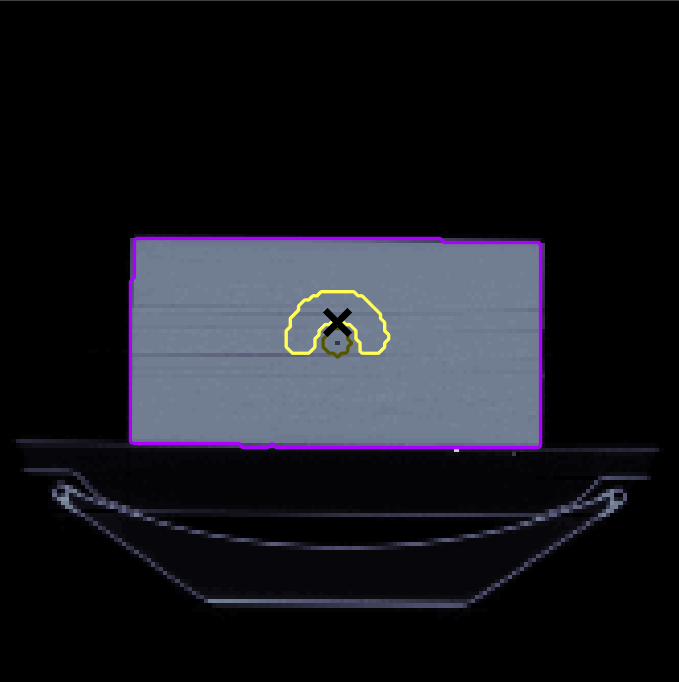
\includegraphics[width=0.33\textwidth]{images/TG119.png}
            \end{figure}
            Sono state quindi simulate diverse particelle incidenti: fotoni, protoni e ioni carbonio; osservando come esse depositino energia nel manichino.
            L'effetto è stato studiato variando il numero di fasci incidenti: impostandoli prima equidistanziati (su 360°) e poi non equidistanziati.
            In seguito si è modificata la risoluzione in larghezza del fascio incidente: cambiando la bixel width nel caso dei 4 fasci di protoni, impostandola dai 5 mm usati in precedenza a 15 mm.
            Infine nel caso di 3 fasci di protoni è stato invertito l'organo a rischio con il target per verificare come variasse la simulazione.
            
            Per la seconda parte si è invece affrontato un caso clinico: ossia il modello Alderson, il quale rappresenta un tumore del testa collo. 
            \begin{figure}[H]
                \centering
                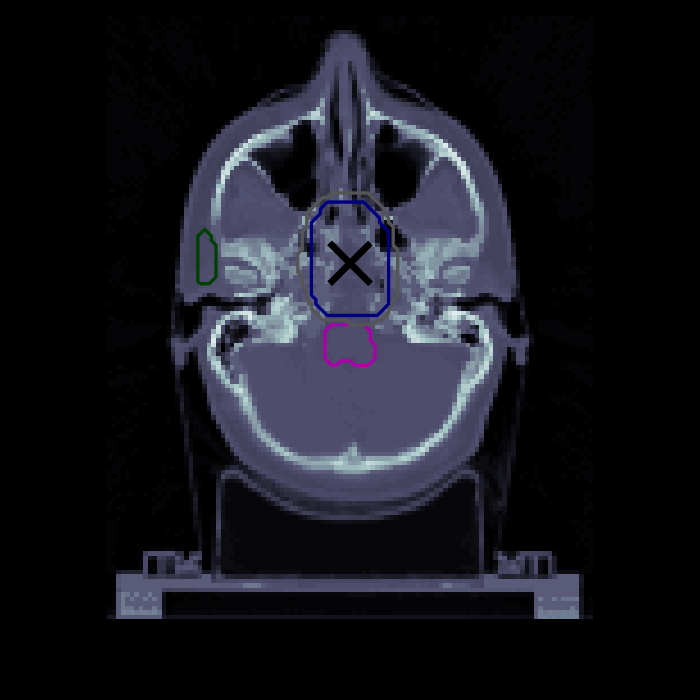
\includegraphics[width=0.33\textwidth]{images/Alderson.png}
            \end{figure}
            Si è studiato un piano di trattamento con fotoni, protoni e ioni carbonio, facendo costruire a MatRad le curve di isodose e il profilo dei fasci.
            Infine si è studiato un possibile malposizionamento del paziente: inserendo manualmente coordinate diverse per l'isocentro e confrontando i dati ottenuti con quelli ricavati precedentemente.

    % -------------------------------------------------------------------
    \section{Dati sperimentali}
        \subsection{1 fascio}
            \subsubsection{Fotoni}
                \begin{figure}[H]
                    \centering
                    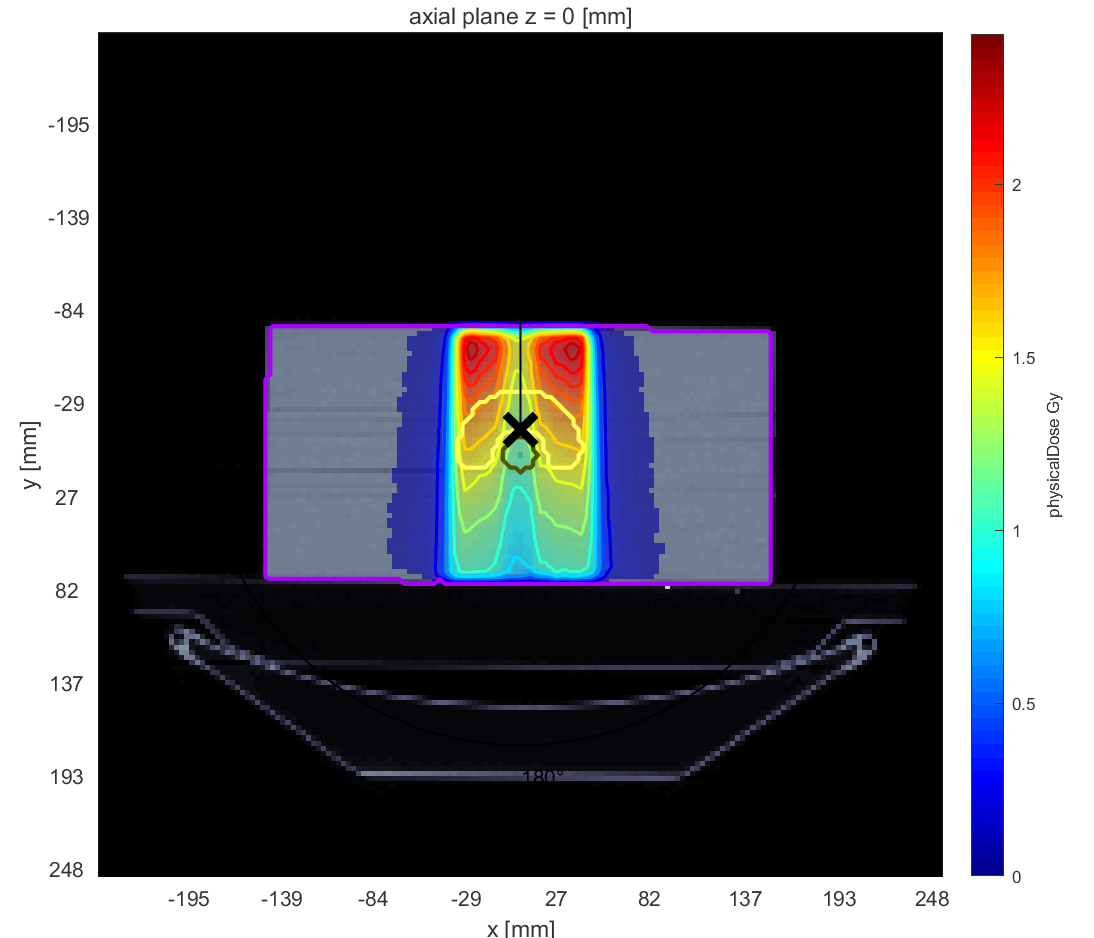
\includegraphics[width=0.6\textwidth]{images/photons/photons_1_intensity.png}
                    \caption{Intensità fascio fotoni}
                    \label{fig:sub_fotoni_1}
                \end{figure}
                \begin{figure}[H]
                    \centering
                    \begin{subfigure}{0.5\textwidth}
                        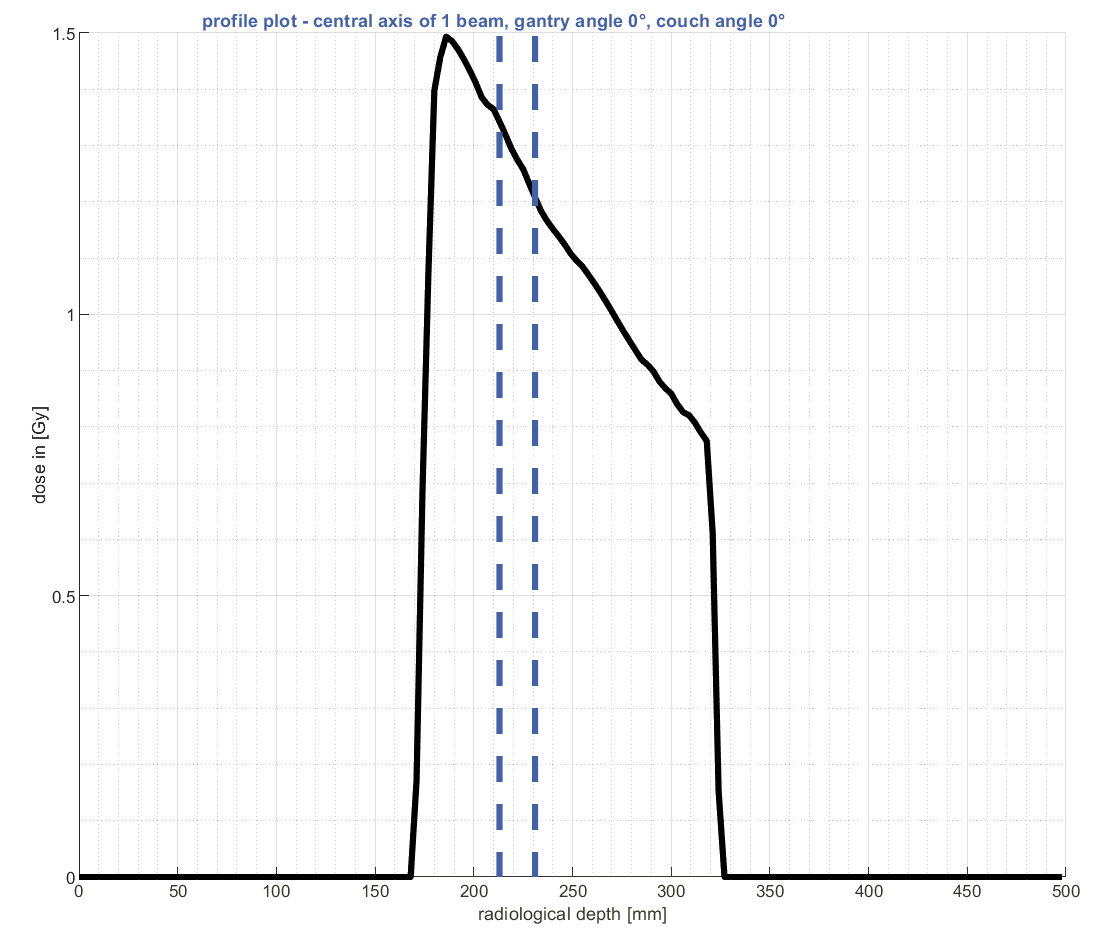
\includegraphics[width=\textwidth]{images/photons/photons_1_depth.png}
                        \caption{Profilo depth}
                        \label{fig:sub_fotoni_1_profile_depth}
                    \end{subfigure}\hfill
                    \begin{subfigure}{0.5\textwidth}
                        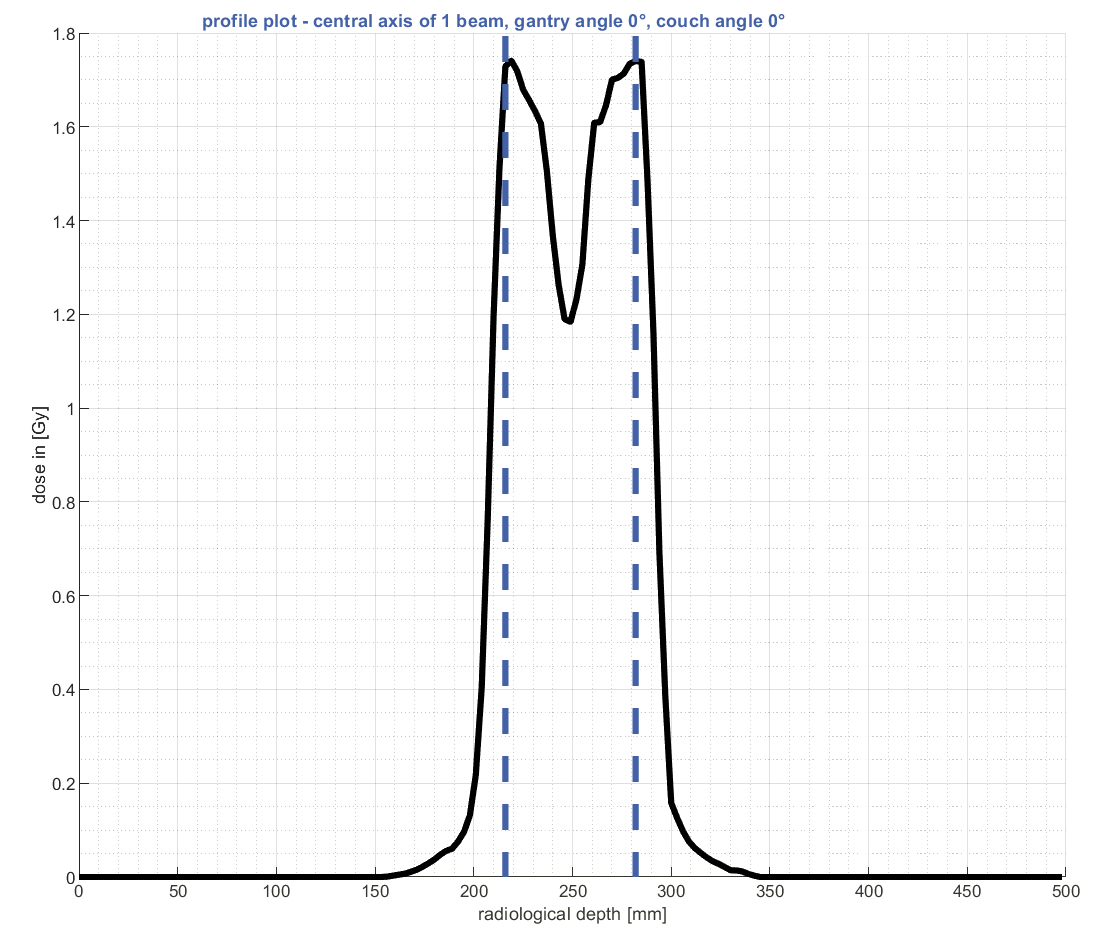
\includegraphics[width=\textwidth]{images/photons/photons_1_lateral.png}
                        \caption{Profilo lateral}
                        \label{fig:sub_fotoni_1_profile_lateral}
                    \end{subfigure}\hfill
                    \caption{Profili del fascio di fotoni}
                    \label{fig:fotoni_1_profiles}
                \end{figure}
                \begin{figure}[H]
                    \centering
                    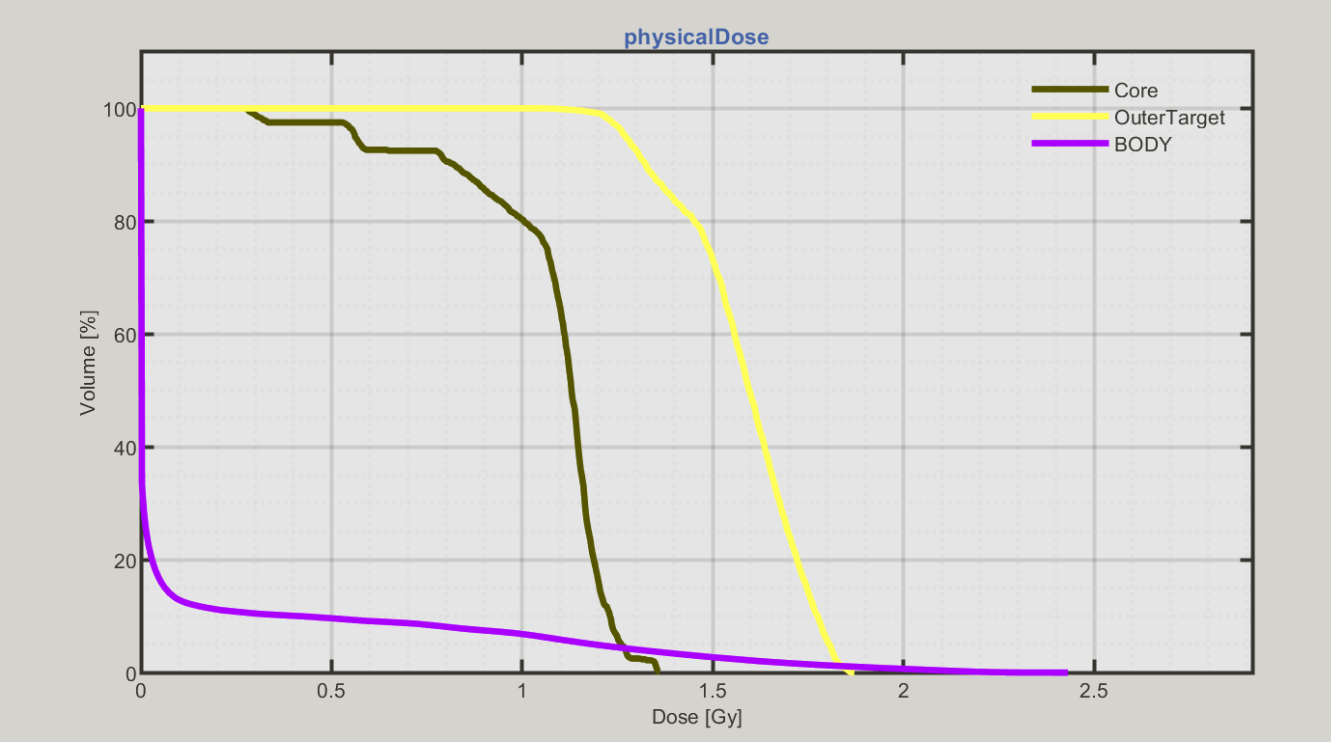
\includegraphics[width=0.6\textwidth]{images/photons/photons_1_DVH_graph.png}
                    \caption{Grafico DVH}
                    \label{fig:fotoni_1_DVH_graph}
                \end{figure}
                \begin{table}[H]
                    \centering
                    \begin{tabular}{
                        l | c | c | c | c | c |
                    }
                    \toprule
                    & Mean & Std & Max & Min & D$_{98}$ \\
                    \midrule
                    Core & 1.0696 & 0.2030 & 1.3614 & 0.2724 & 0.3207 \\
                    Outer target & 1.5769 & 0.1598 & 1.8734 & 1.0588 & 1.2279 \\
                    Body & 0.1345 & 0.3941 & 2.4321 & 0 & 0 \\
                    \bottomrule
                    \end{tabular}
                    \caption{Dati ottenuti dalle curve di isodose (unità di misura della tabella [\unit{\gray}])}
                    \label{tab:dati_prima_misura_fotoni}
                \end{table}

            \subsubsection{Protoni}
                % Protoni 1
                \begin{figure}[H]
                    \centering
                    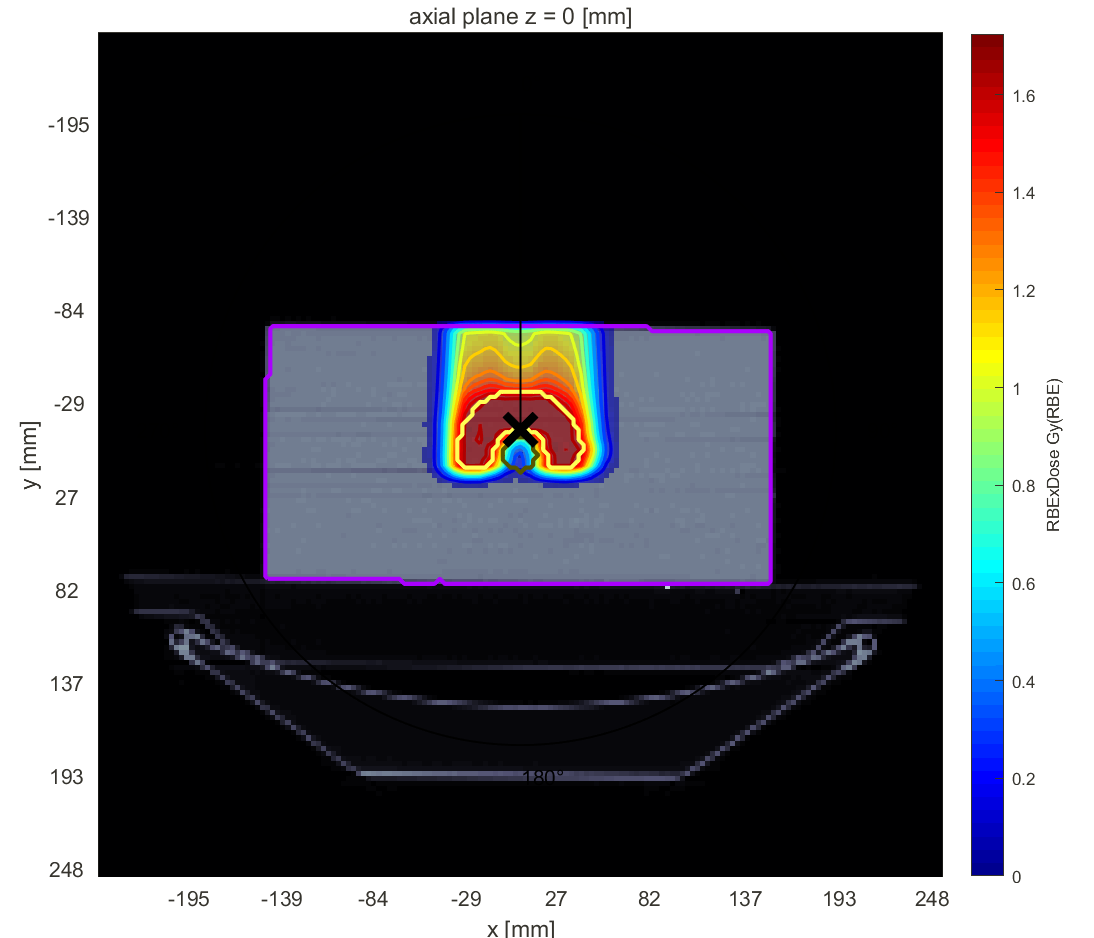
\includegraphics[width=0.6\textwidth]{images/protons/protons_1_intensity.png}
                    \caption{Intensità fascio protoni}
                    \label{fig:sub_protoni_1}
                \end{figure}
                \begin{figure}[H]
                    \centering
                    \begin{subfigure}{0.5\textwidth}
                        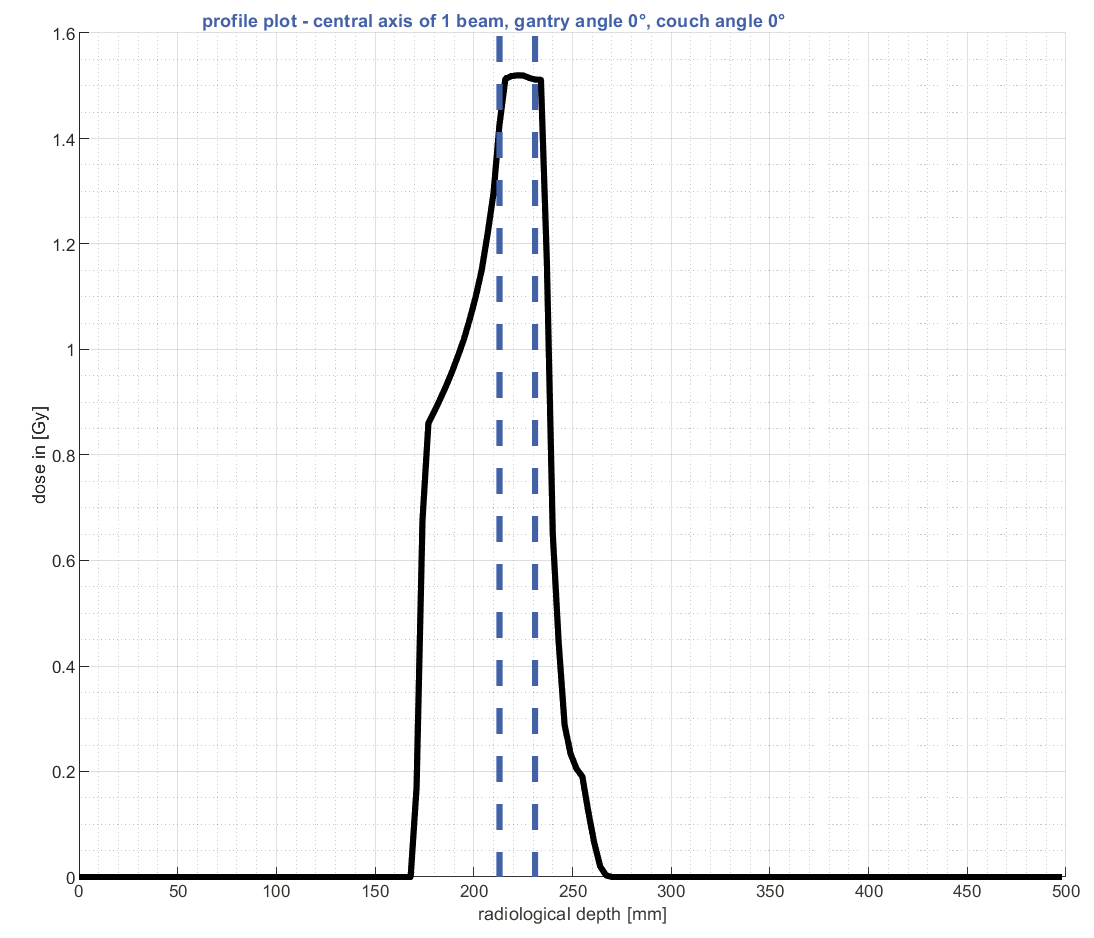
\includegraphics[width=\textwidth]{images/protons/protons_1_depth.png}
                        \caption{Profilo depth}
                        \label{fig:sub_protoni_1_profile_depth}
                    \end{subfigure}\hfill
                    \begin{subfigure}{0.5\textwidth}
                        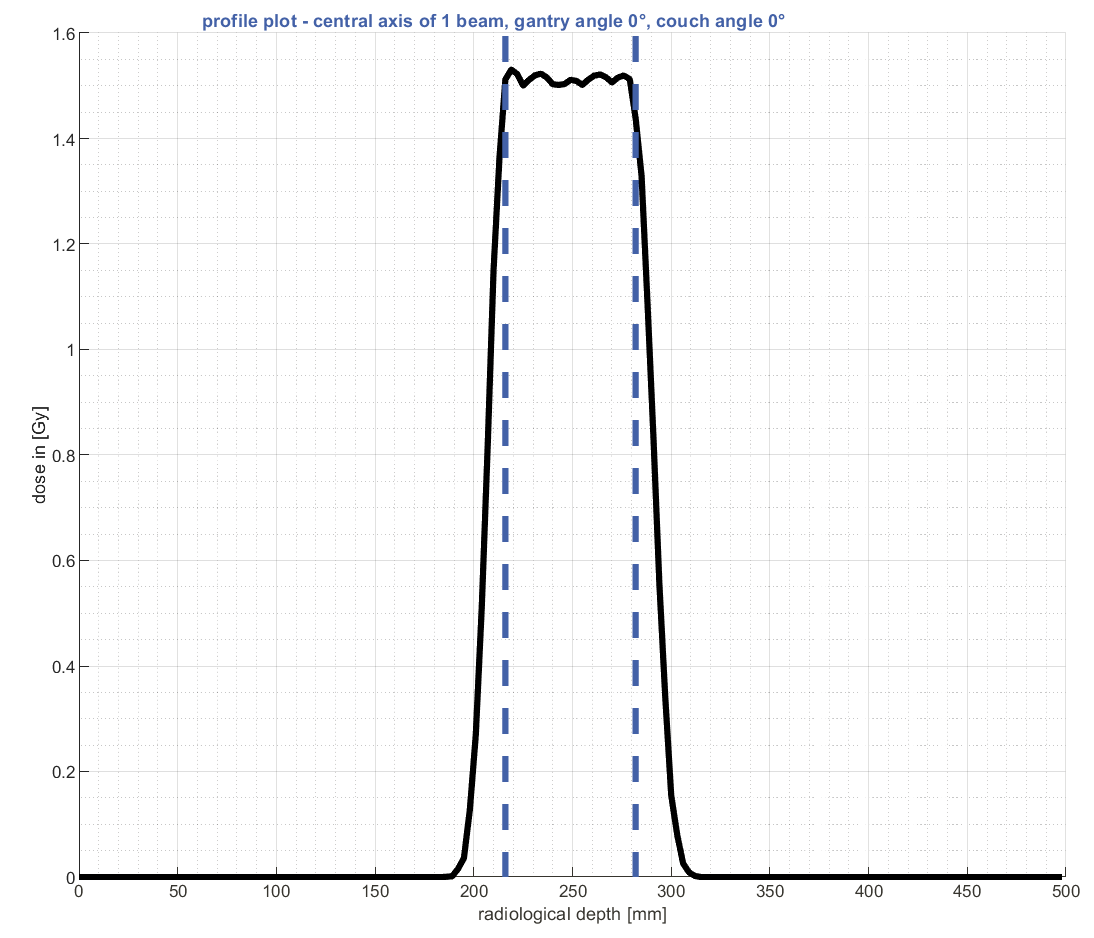
\includegraphics[width=\textwidth]{images/protons/protons_1_lateral.png}
                        \caption{Profilo lateral}
                        \label{fig:sub_protoni_1_profile_lateral}
                    \end{subfigure}\hfill
                    \caption{Profili del fascio di protoni}
                    \label{fig:protoni_1_profiles}
                \end{figure}
                \begin{figure}[H]
                    \centering
                    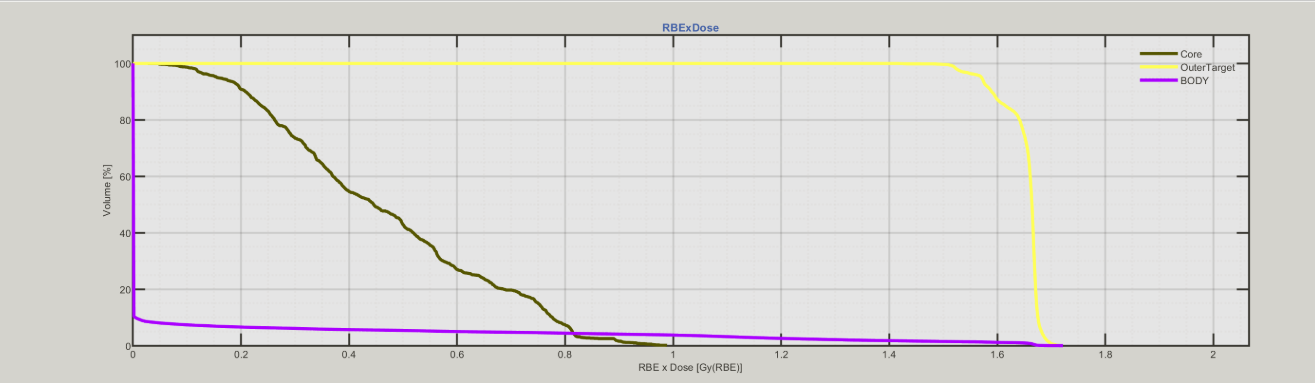
\includegraphics[width=0.6\textwidth]{images/protons/protons_1_DVH_graph.png}
                    \caption{Grafico DVH}
                    \label{fig:protoni_1_DVH_graph}
                \end{figure}
                \begin{table}[H]
                    \centering                    
                    \begin{tabular}{
                        l | c | c | c | c | c |
                    }
                    \toprule
                    & Mean & Std & Max & Min & D$_{98}$ \\
                    \midrule
                    Core & 0.4677 & 0.2135 & 0.9888 & 0.0281 & 0.1173 \\
                    Outer target & 1.6502 & 0.0376 & 1.7222 & 1.4190 & 1.5253 \\
                    Body & 0.0699 & 0.2823 & 1.7222 & 0 & 0 \\
                    \bottomrule
                    \end{tabular}
                    \caption{Dati ottenuti dalle curve di isodose (unità di misura della tabella [\unit{\gray}])}
                    \label{tab:dati_prima_misura_protoni}
                \end{table}

            \subsubsection{Ioni carbonio}
                % Carbonio 1
                \begin{figure}[H]
                    \centering
                    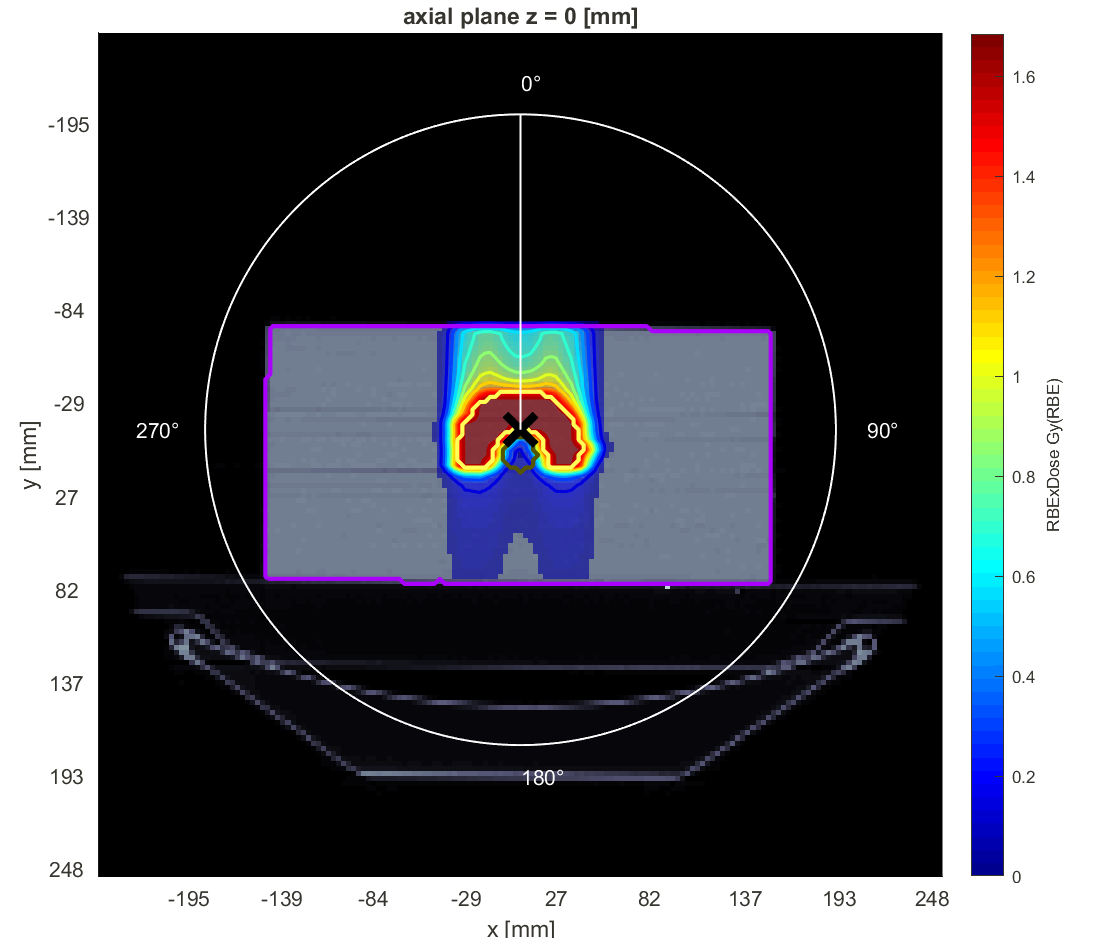
\includegraphics[width=0.6\textwidth]{images/carbon/carbon_1_intensity.png}
                    \caption{Intensità fascio ioni carbonio}
                    \label{fig:sub_carbonio_1}
                \end{figure}
                \begin{figure}[H]
                    \centering
                    \begin{subfigure}{0.5\textwidth}
                        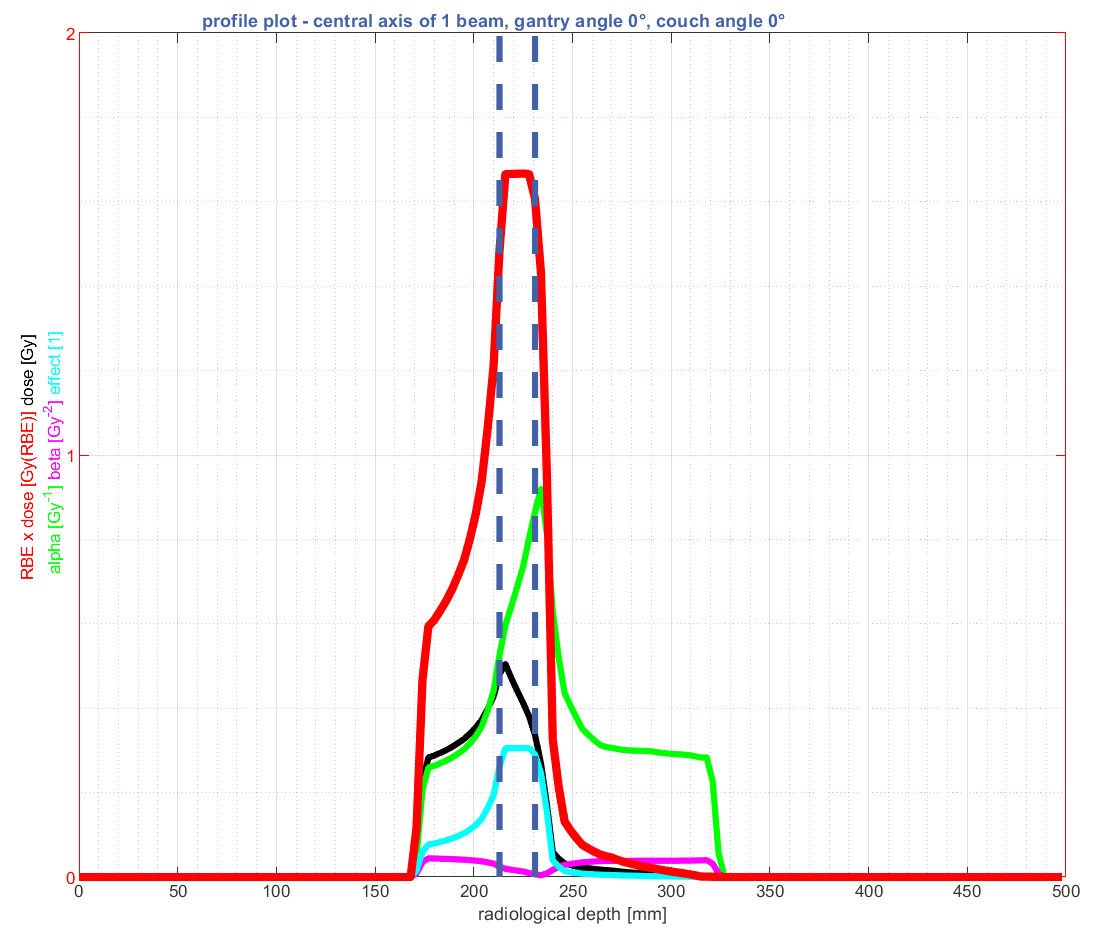
\includegraphics[width=\textwidth]{images/carbon/carbon_1_depth.png}
                        \caption{Profilo depth}
                        \label{fig:sub_carbonio_1_profile_depth}
                    \end{subfigure}\hfill
                    \begin{subfigure}{0.5\textwidth}
                        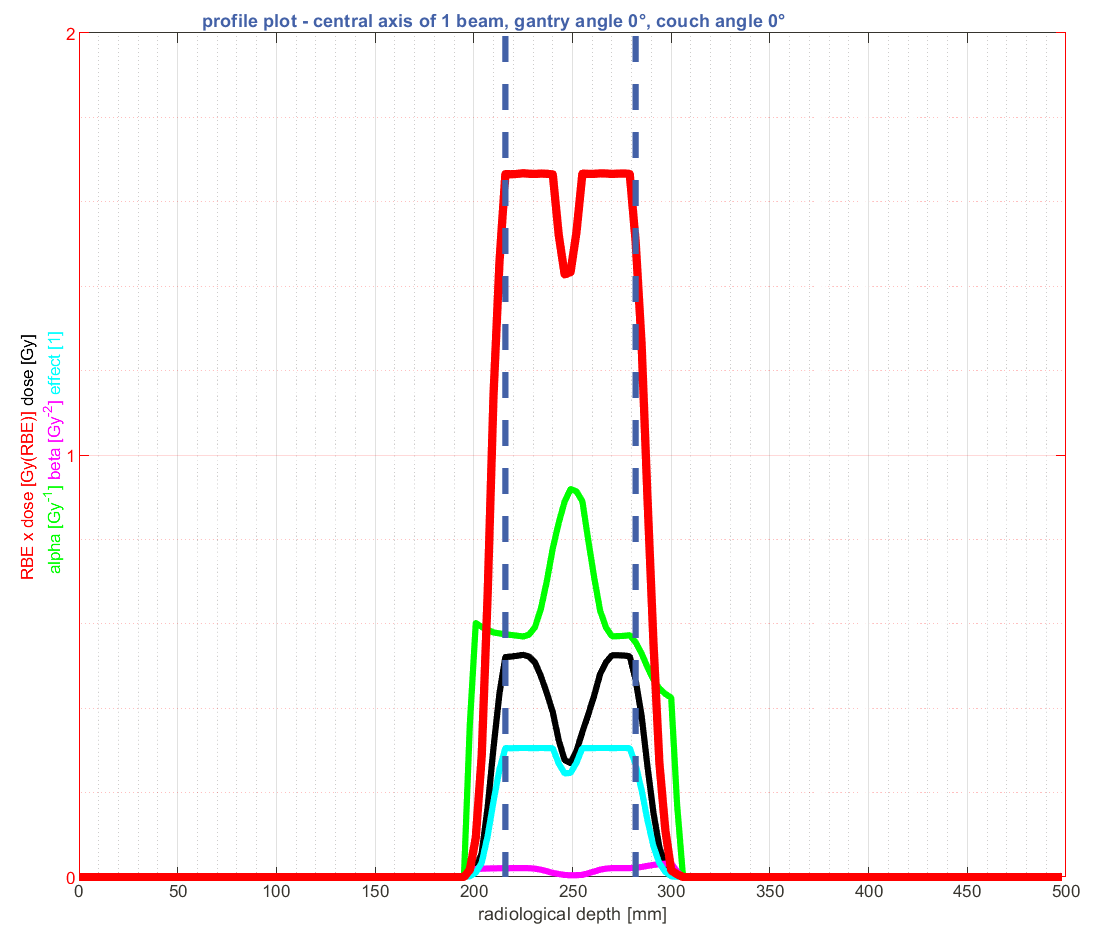
\includegraphics[width=\textwidth]{images/carbon/carbon_1_lateral.png}
                        \caption{Profilo lateral}
                        \label{fig:sub_carbonio_1_profile_lateral}
                    \end{subfigure}\hfill
                    \caption{Profili del fascio di ioni carbonio}
                    \label{fig:carbonio_1_profiles}
                \end{figure}
                \begin{figure}[H]
                    \centering
                    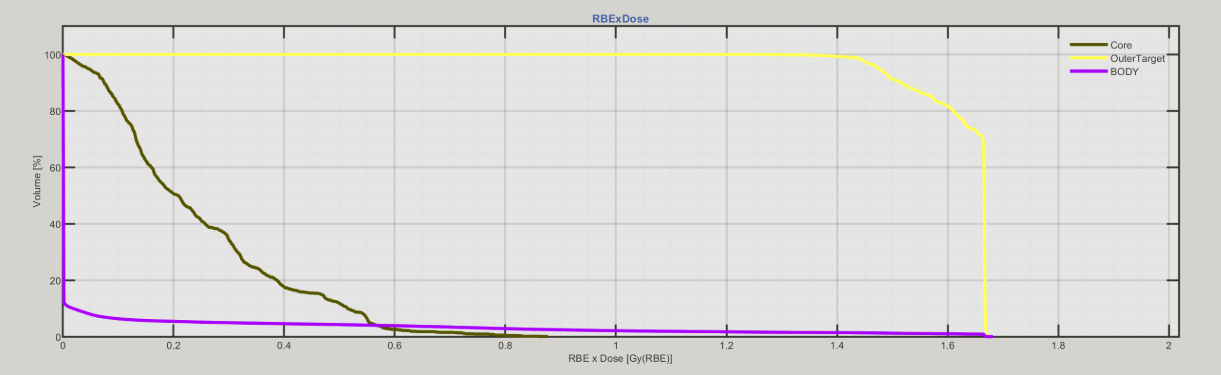
\includegraphics[width=0.6\textwidth]{images/carbon/carbon_1_DVH_graph.png}
                    \caption{Grafico DVH}
                    \label{fig:carbon_1_DVH_graph}
                \end{figure}
                \begin{table}[H]
                    \centering
                    \label{tab:dati_prima_misura_carbonio}
                    \begin{tabular}{
                        l | c | c | c | c | c |
                    }
                    \toprule
                    & Mean & Std & Max & Min & D$_{98}$ \\
                    \midrule
                    Core & 0.2491 & 0.1678 & 0.8773 & 0.0044 & 0.0199 \\
                    Outer target & 1.6336 & 0.0656 & 1.6824 & 1.2518 & 1.4449 \\
                    Body & 0.0540 & 0.2399 & 1.6824 & 0 & 0 \\
                    \bottomrule
                    \end{tabular}
                    \caption{Dati ottenuti dalle curve di isodose (unità di misura della tabella [\unit{\gray}])}
                \end{table}            

        \subsection{3 fasci equidistanziati}
            \subsubsection{Fotoni}
                \begin{figure}[H]
                    \centering
                    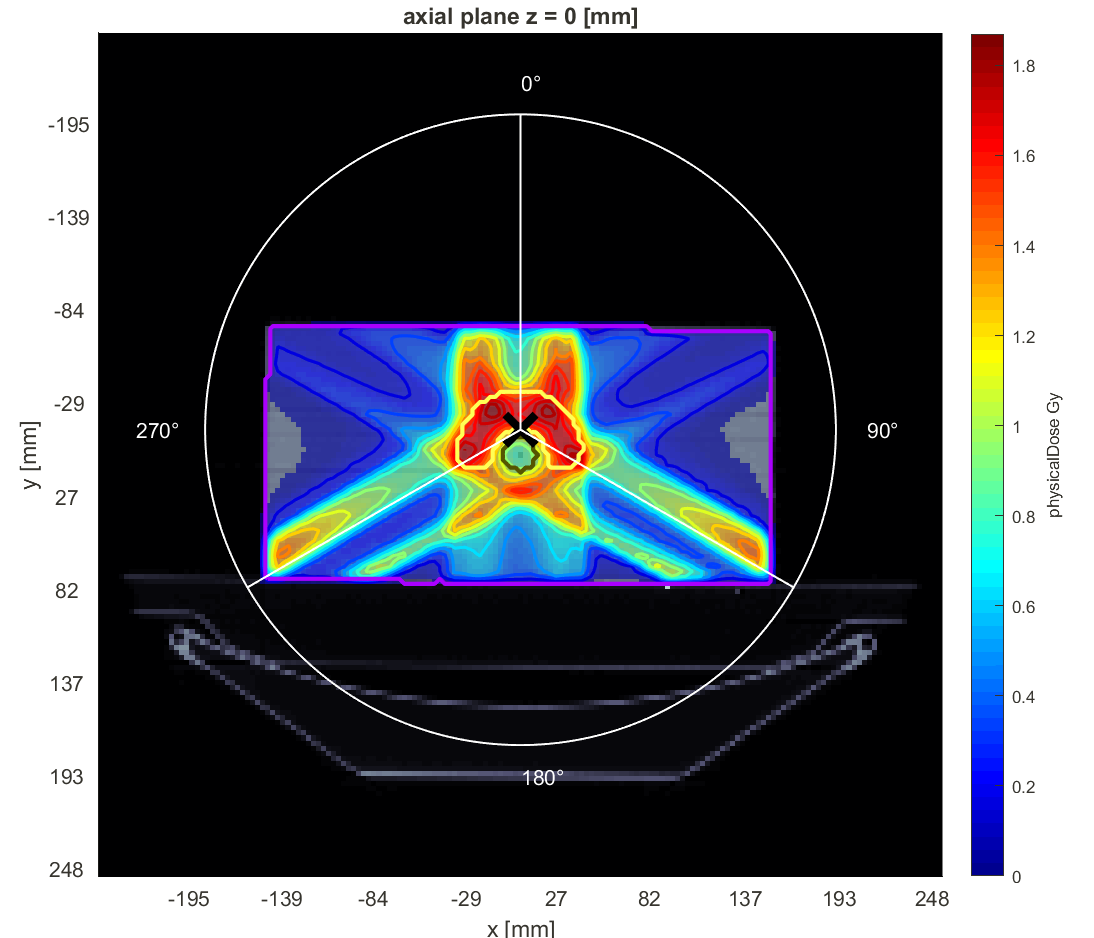
\includegraphics[width=0.6\textwidth]{images/photons/photons_3_eq_intensity.png}
                    \caption{Intensità fasci fotoni}
                    \label{fig:sub_fotoni_3}
                \end{figure}
                \begin{figure}[H]
                    \centering
                    \begin{subfigure}{0.5\textwidth}
                        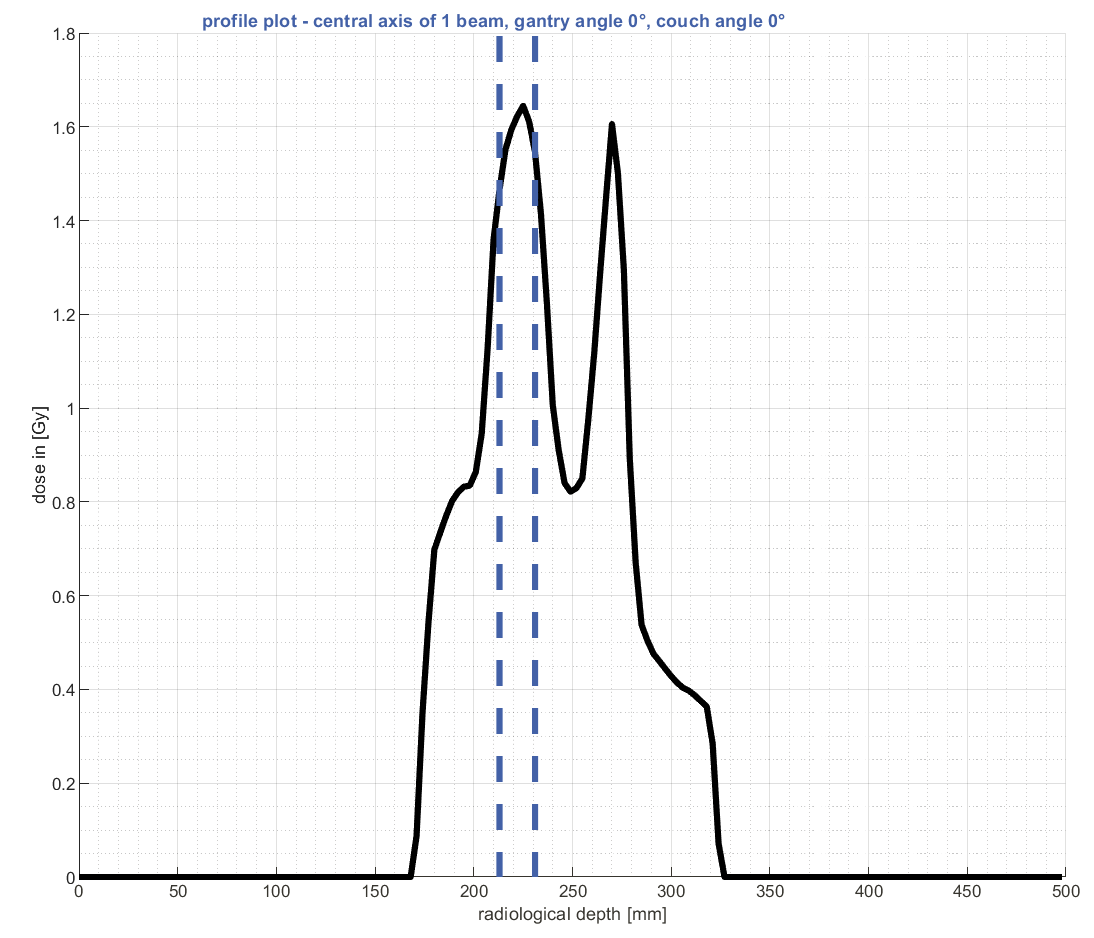
\includegraphics[width=\textwidth]{images/photons/photons_3_eq_depth.png}
                        \caption{Profilo depth}
                        \label{fig:sub_fotoni_3_profile_depth}
                    \end{subfigure}\hfill
                    \begin{subfigure}{0.5\textwidth}
                        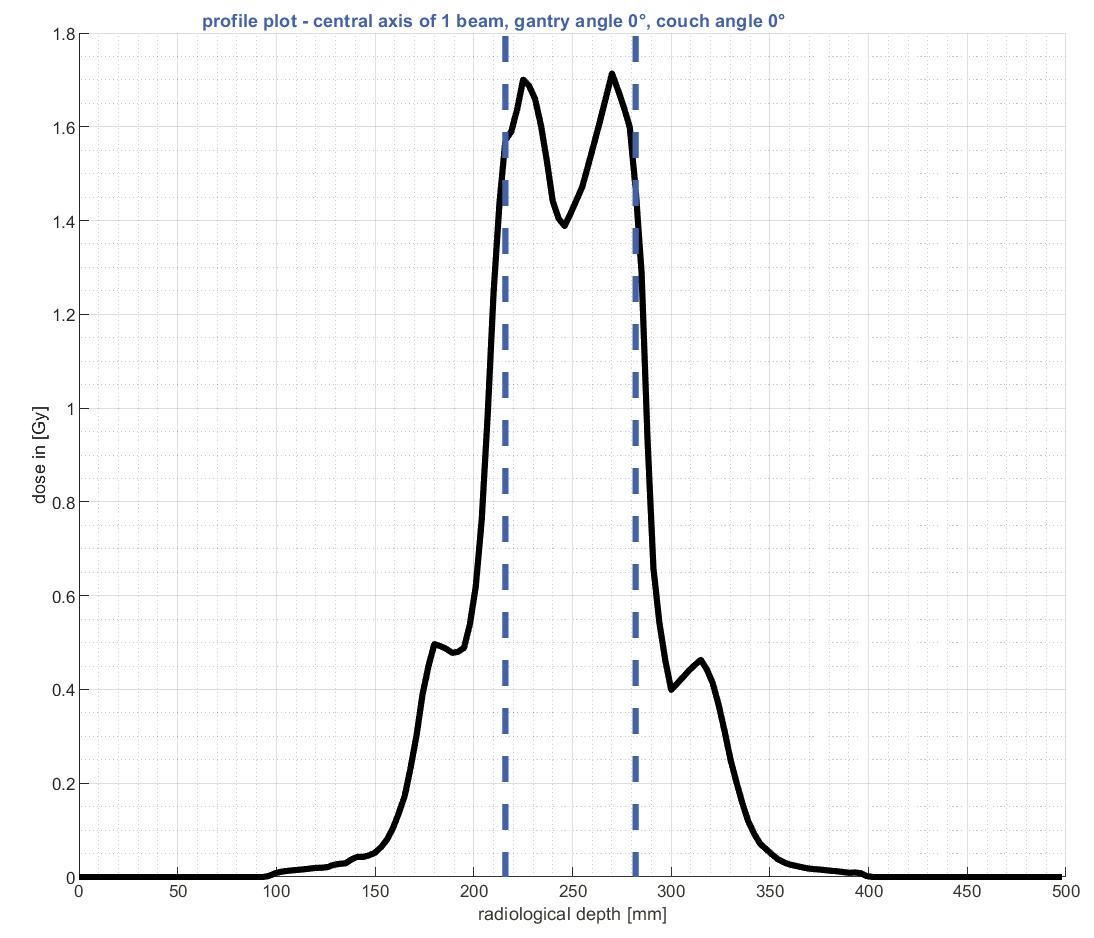
\includegraphics[width=\textwidth]{images/photons/photons_3_eq_lateral.png}
                        \caption{Profilo lateral}
                        \label{fig:sub_fotoni_3_profile_lateral}
                    \end{subfigure}\hfill
                    \caption{Profili dei 3 fasci di fotoni}
                    \label{fig:fotoni_3_profiles}
                \end{figure}
                \begin{figure}[H]
                    \centering
                    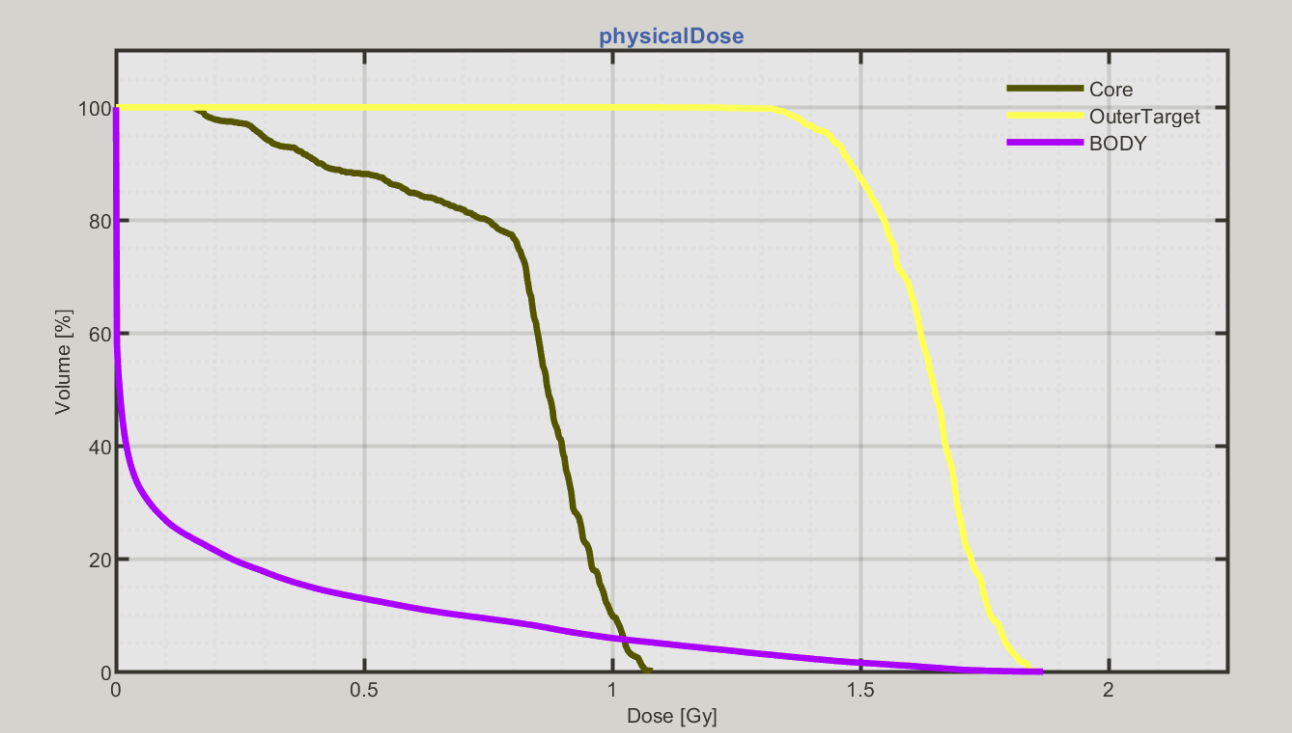
\includegraphics[width=0.6\textwidth]{images/photons/photons_3_eq_DVH_graph.png}
                    \caption{Grafico DVH}
                    \label{fig:fotoni_3_DVH_graph}
                \end{figure}
                \begin{table}[H]
                    \centering
                    \label{tab:dati_seconda_misura_fotoni}
                    \begin{tabular}{
                        l | c | c | c | c | c |
                    }
                    \toprule
                    & Mean & Std & Max & Min & D$_{98}$ \\
                    \midrule
                    Core & 0.8125 & 0.2108 & 1.0809 & 0.1559 & 0.1959 \\
                    Outer target & 1.6336 & 0.1081 & 1.8678 & 1.1082 & 1.3748 \\
                    Body & 0.1752 & 0.3610 & 1.8678 & 0 & 0 \\
                    \bottomrule
                    \end{tabular}
                    \caption{Dati ottenuti dalle curve di isodose (unità di misura della tabella [\unit{\gray}])}
                \end{table}

            \subsubsection{Protoni}
                \begin{figure}[H]
                    \centering
                    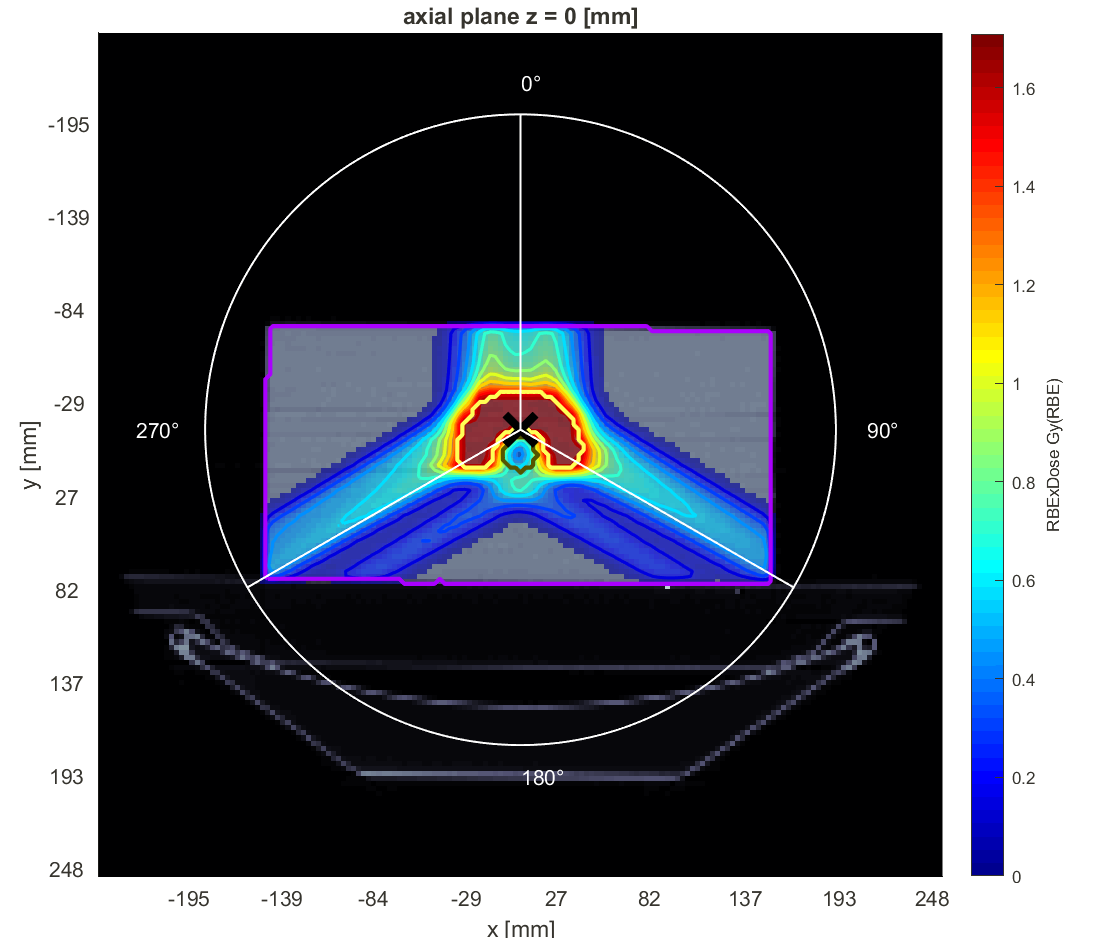
\includegraphics[width=0.6\textwidth]{images/protons/protons_3_eq_intensity.png}
                    \caption{Intensità fasci protoni}
                    \label{fig:sub_protoni_3}
                \end{figure}
                \begin{figure}[H]
                    \centering
                    \begin{subfigure}{0.5\textwidth}
                        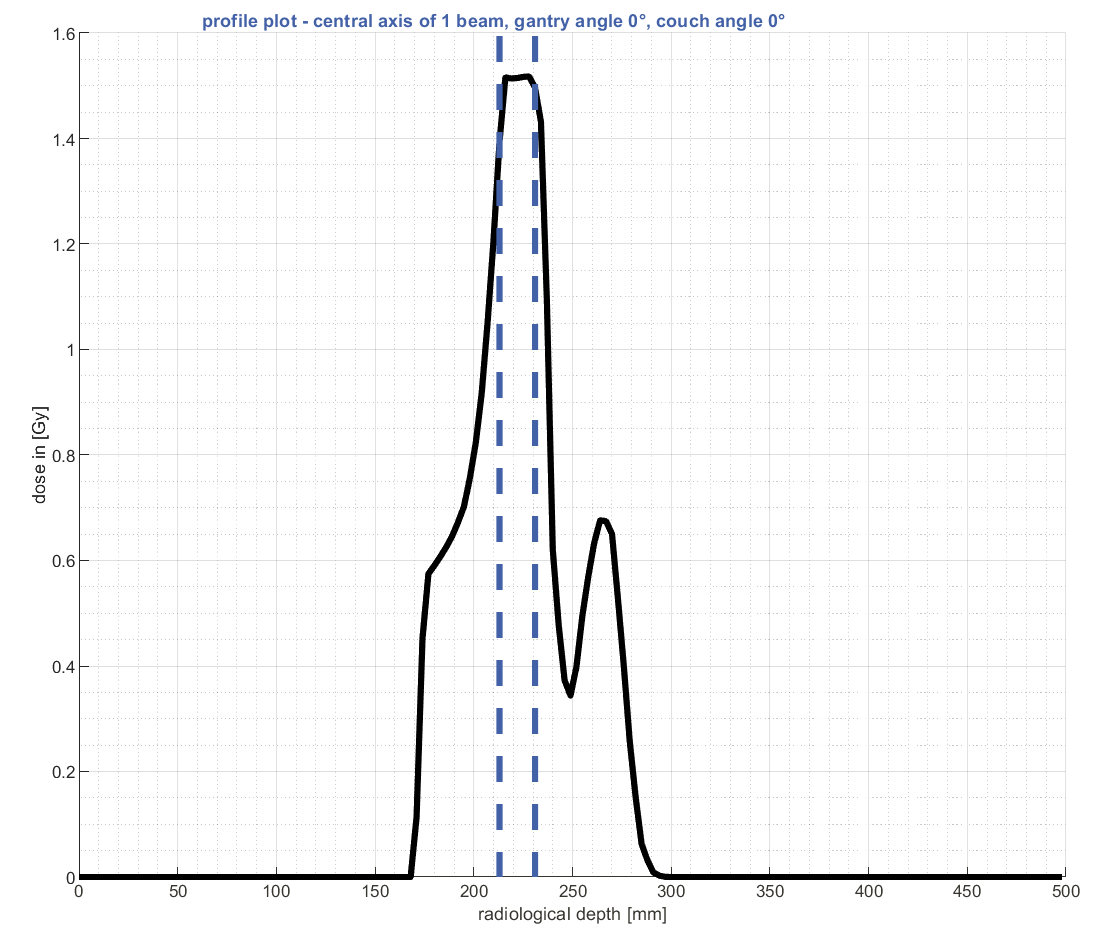
\includegraphics[width=\textwidth]{images/protons/protons_3_eq_depth.png}
                        \caption{Profilo depth}
                        \label{fig:sub_protoni_3_profile_depth}
                    \end{subfigure}\hfill
                    \begin{subfigure}{0.5\textwidth}
                        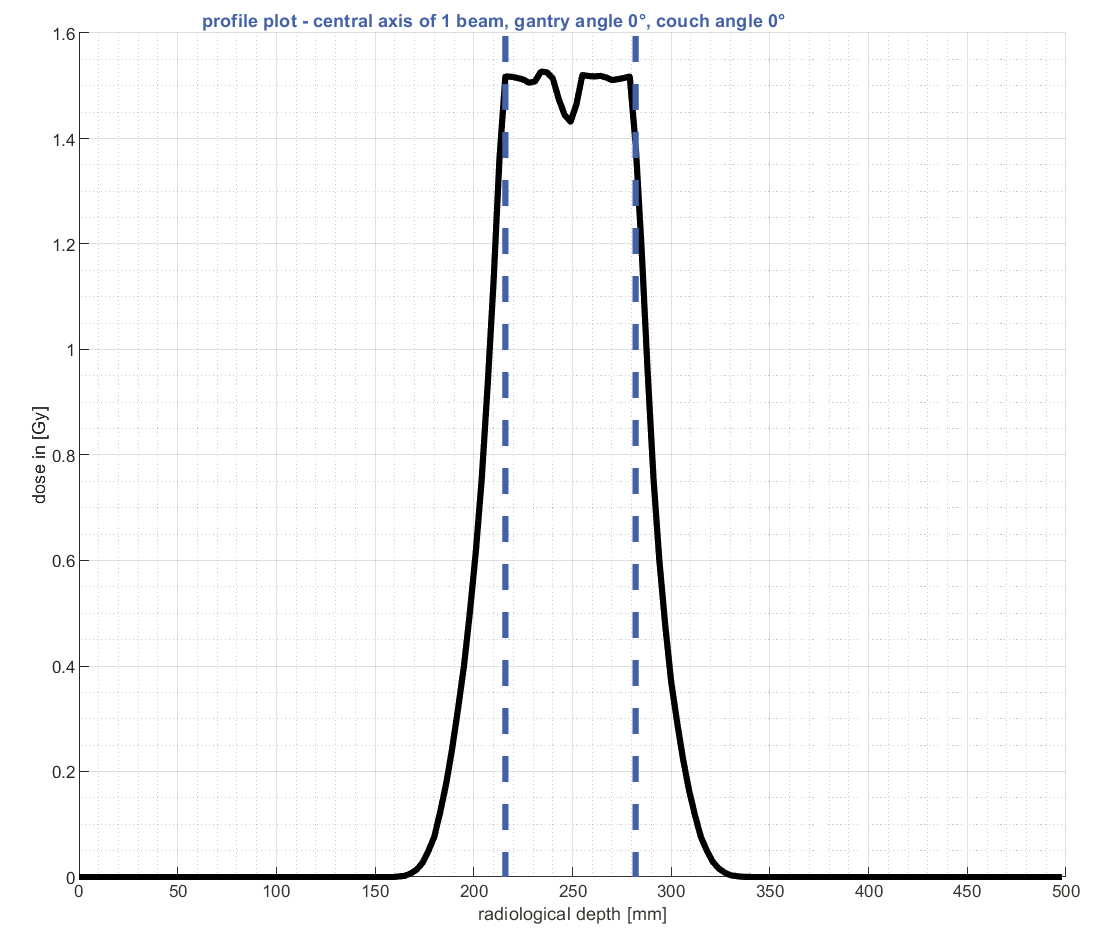
\includegraphics[width=\textwidth]{images/protons/protons_3_eq_lateral.png}
                        \caption{Profilo lateral}
                        \label{fig:sub_protoni_3_profile_lateral}
                    \end{subfigure}\hfill
                    \caption{Profili dei 3 fasci di protoni}
                    \label{fig:protoni_3_profiles}
                \end{figure}
                \begin{figure}[H]
                    \centering
                    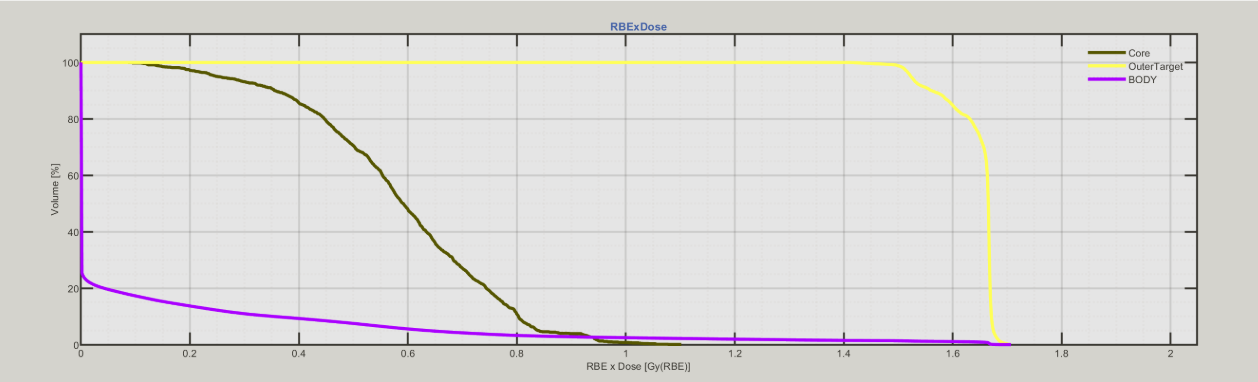
\includegraphics[width=0.6\textwidth]{images/protons/protons_3_eq_DVH_graph.png}
                    \caption{Grafico DVH}
                    \label{fig:protoni_3_DVH_graph}
                \end{figure}
                \begin{table}[H]
                    \centering
                    \label{tab:dati_seconda_misura_protoni}
                    \begin{tabular}{
                        l | c | c | c | c | c |
                    }
                    \toprule
                    & Mean & Std & Max & Min & D$_{98}$ \\
                    \midrule
                    Core & 0.5870 & 0.1782 & 1.1021 & 0.0866 & 0.1855 \\
                    Outer target & 1.6439 & 0.0473 & 1.7074 & 1.3896 & 1.5096 \\
                    Body & 0.0978 & 0.2739 & 1.7074 & 0 & 0 \\
                    \bottomrule
                    \end{tabular}
                    \caption{Dati ottenuti dalle curve di isodose (unità di misura della tabella [\unit{\gray}])}
                \end{table}

            \subsubsection{Ioni carbonio}
                \begin{figure}[H]
                    \centering
                    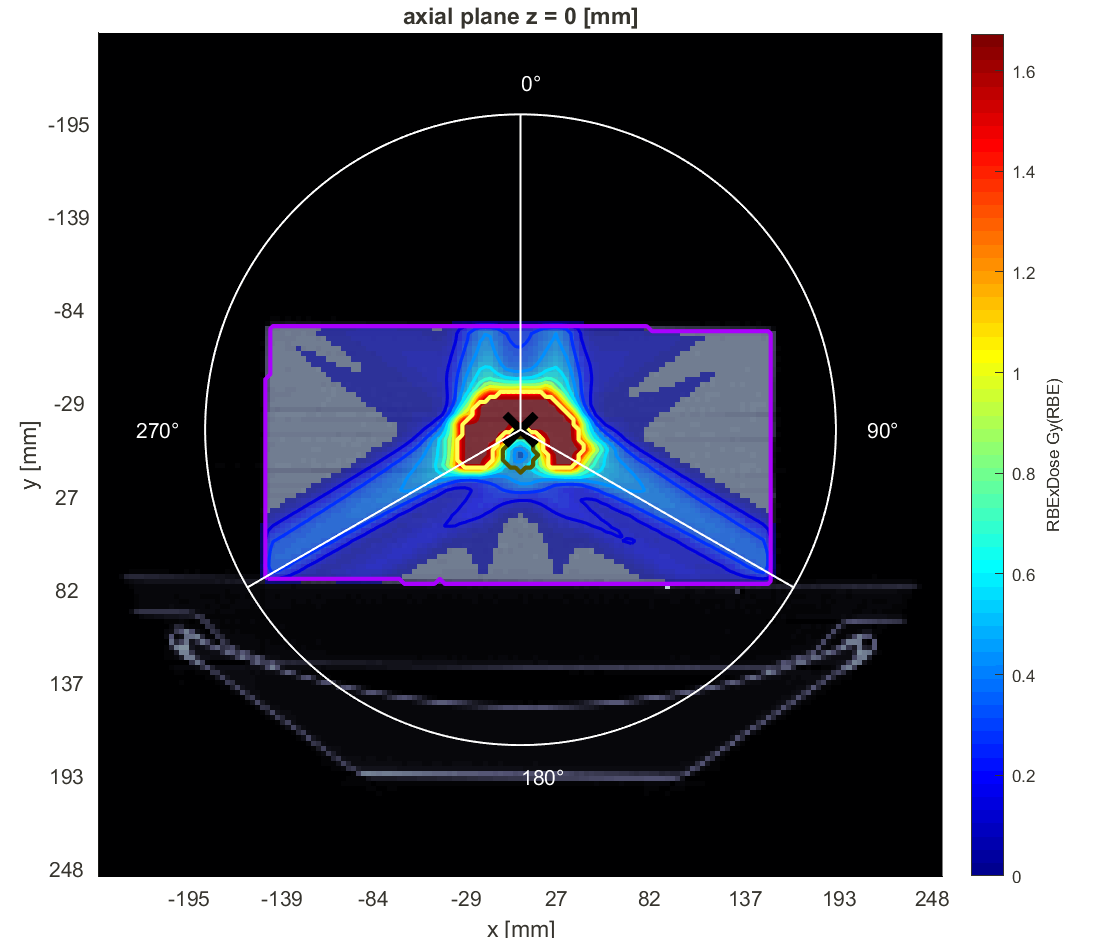
\includegraphics[width=0.6\textwidth]{images/carbon/carbon_3_eq_intensity.png}
                    \caption{Intensità ioni carbonio}
                    \label{fig:sub_carbonio_3}
                \end{figure}
                \begin{figure}[H]
                    \centering
                    \begin{subfigure}{0.5\textwidth}
                        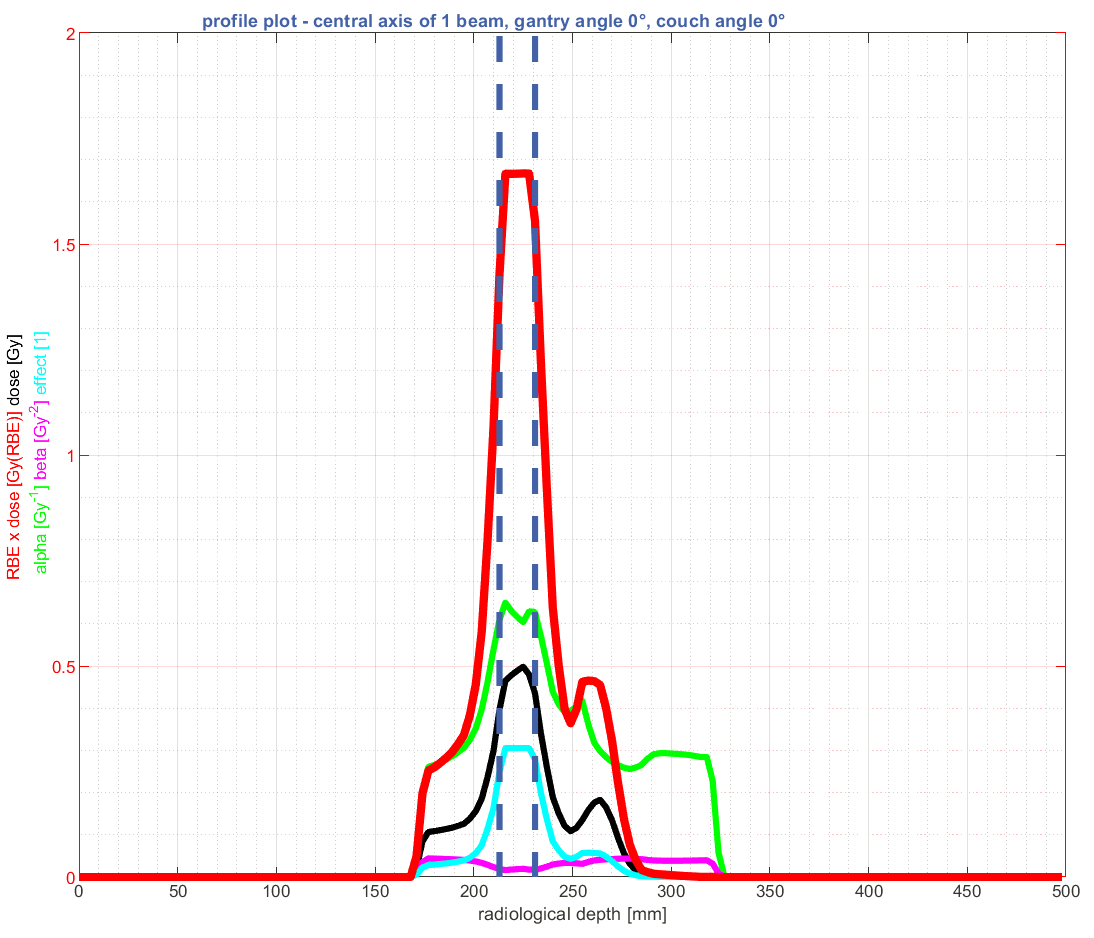
\includegraphics[width=\textwidth]{images/carbon/carbon_3_eq_depth.png}
                        \caption{Profilo depth}
                        \label{fig:sub_carbonio_3_profile_depth}
                    \end{subfigure}\hfill
                    \begin{subfigure}{0.5\textwidth}
                        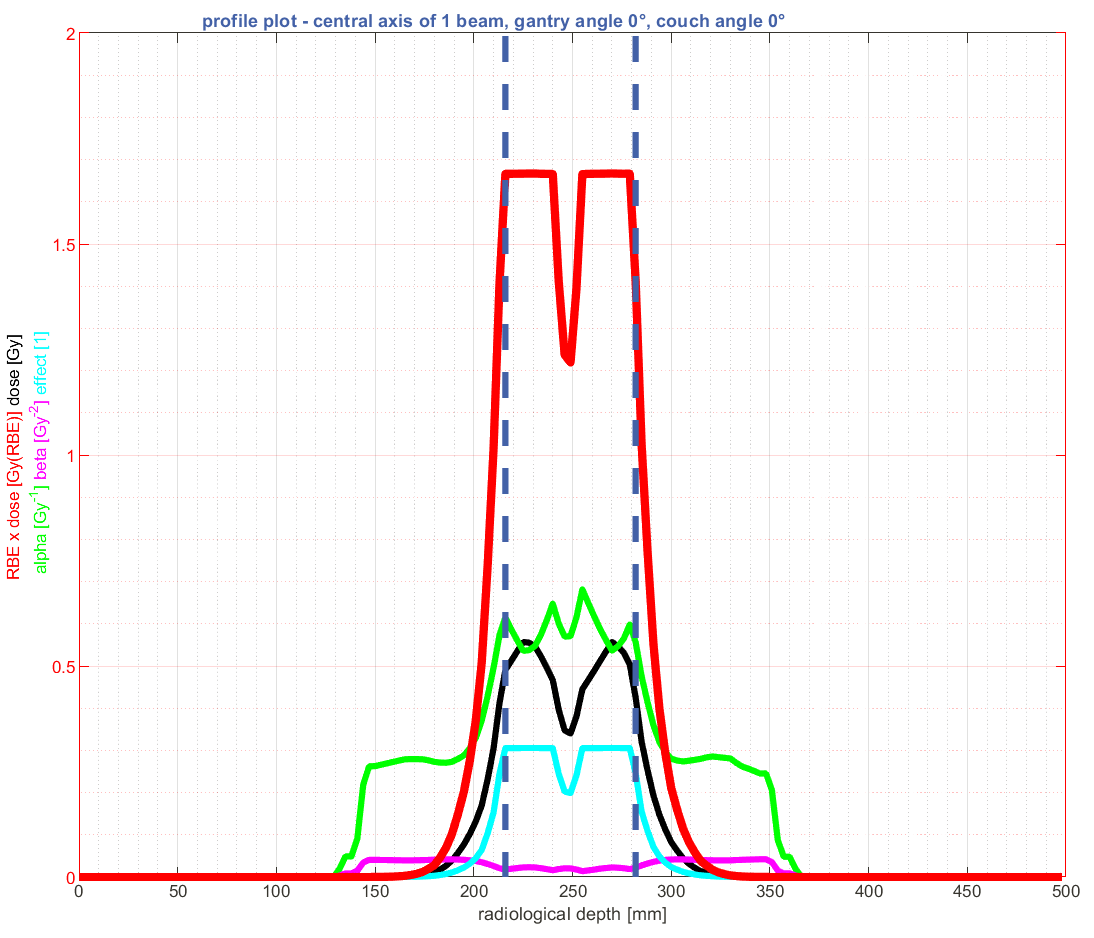
\includegraphics[width=\textwidth]{images/carbon/carbon_3_eq_lateral.png}
                        \caption{Profilo lateral}
                        \label{fig:sub_carbonio_3_profile_lateral}
                    \end{subfigure}\hfill
                    \caption{Profili dei 3 fasci di ioni carbonio}
                    \label{fig:carbonio_3_profiles}
                \end{figure}
                \begin{figure}[H]
                    \centering
                    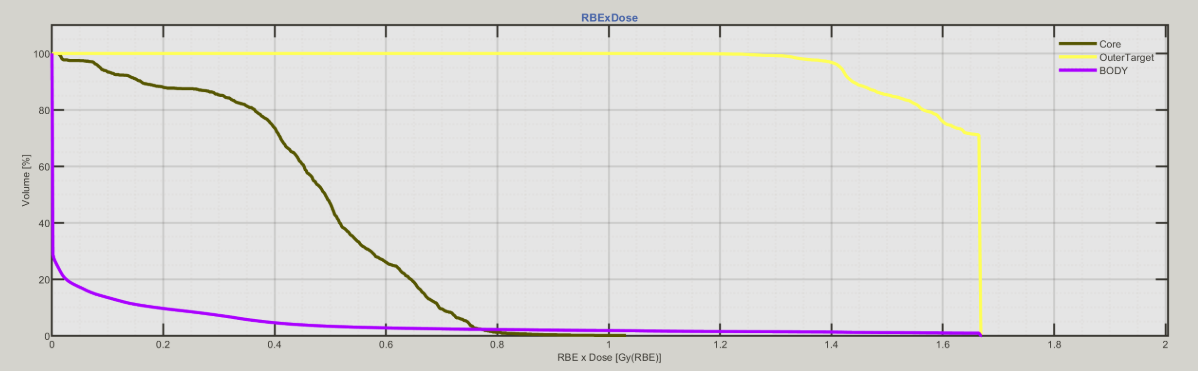
\includegraphics[width=0.6\textwidth]{images/carbon/carbon_3_eq_DVH_graph.png}
                    \caption{Grafico DVH}
                    \label{fig:carbon_3_DVH_graph}
                \end{figure}
                \begin{table}[H]
                    \centering
                    \label{tab:dati_seconda_misura_carbonio}
                    \begin{tabular}{
                        l | c | c | c | c | c |
                    }
                    \toprule
                    & Mean & Std & Max & Min & D$_{98}$ \\
                    \midrule
                    Core & 0.4739 & 0.1862 & 1.0310 & 0.0106 & 0.0192 \\
                    Outer target & 1.6178 & 0.0931 & 1.6709 & 1.0026 & 1.3515 \\
                    Body & 0.0680 & 0.2275 & 1.6709 & 0 & 0 \\
                    \bottomrule
                    \end{tabular}
                    \caption{Dati ottenuti dalle curve di isodose (unità di misura della tabella [\unit{\gray}])}
                \end{table}

        \subsection{3 fasci non equidistanziati}
            \subsubsection{Fotoni}
                \begin{figure}[H]
                    \centering
                    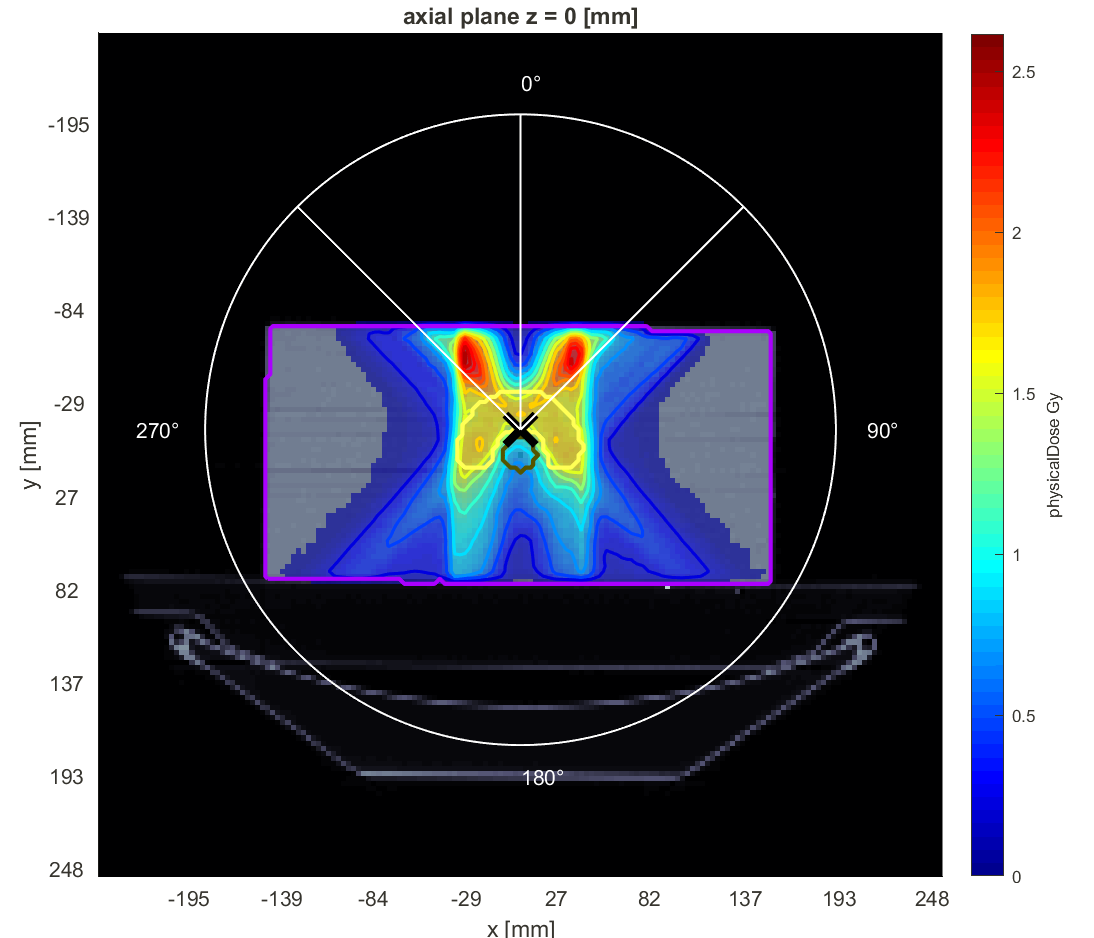
\includegraphics[width=0.6\textwidth]{images/photons/photons_3_noeq_intensity.png}
                    \caption{Fotoni}
                    \label{fig:sub_fotoni_3_no}
                \end{figure}
                \begin{figure}[H]
                    \centering
                    \begin{subfigure}{0.5\textwidth}
                        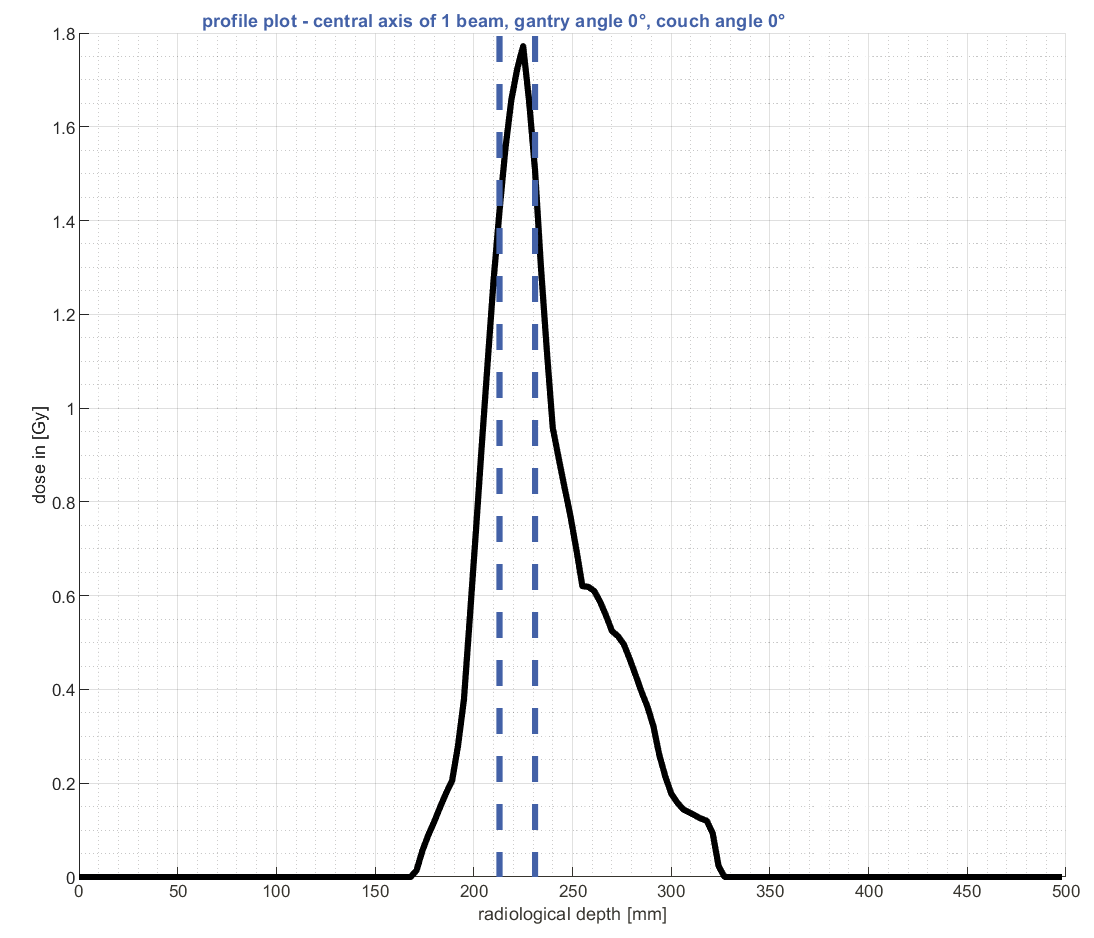
\includegraphics[width=\textwidth]{images/photons/photons_3_noeq_depth.png}
                        \caption{Profilo depth}
                        \label{fig:sub_fotoni_3_no_profile_depth}
                    \end{subfigure}\hfill
                    \begin{subfigure}{0.5\textwidth}
                        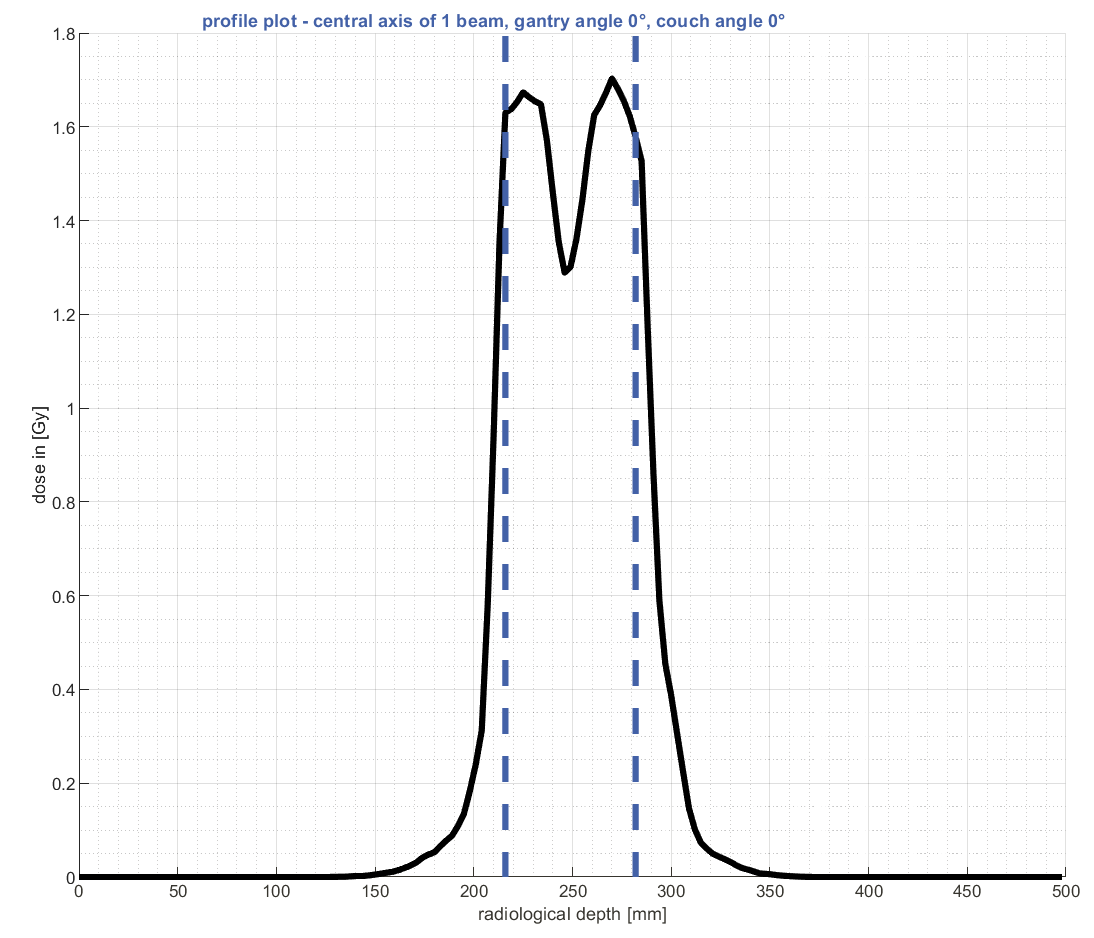
\includegraphics[width=\textwidth]{images/photons/photons_3_noeq_lateral.png}
                        \caption{Profilo lateral}
                        \label{fig:sub_fotoni_3_no_profile_lateral}
                    \end{subfigure}\hfill
                    \caption{Profili del fascio di fotoni}
                    \label{fig:fotoni_3_no_profiles}
                \end{figure}
                \begin{figure}[H]
                    \centering
                    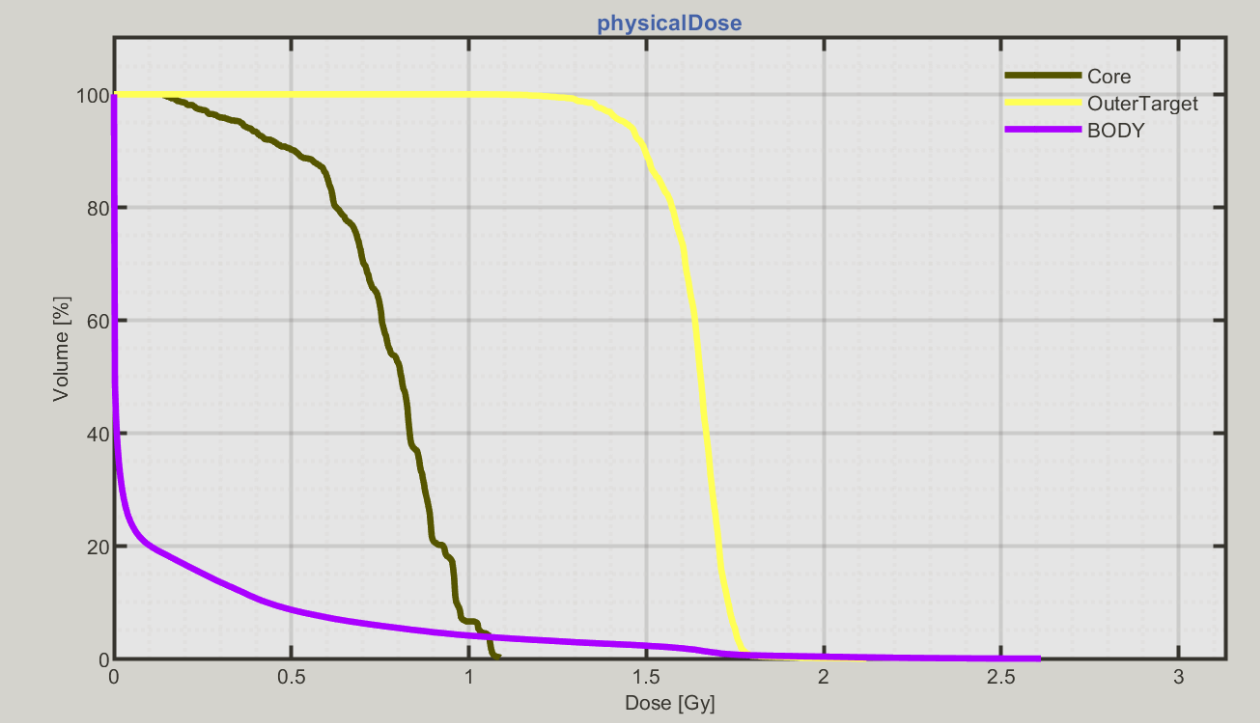
\includegraphics[width=0.6\textwidth]{images/photons/photons_3_noeq_DVH_graph.png}
                    \caption{Grafico DVH}
                    \label{fig:fotoni_3_no_DVH_graph}
                \end{figure}
                \begin{table}[H]
                    \centering
                    \label{tab:dati_terza_misura_fotoni}
                    \begin{tabular}{
                        l | c | c | c | c | c |
                    }
                    \toprule
                    & Mean & Std & Max & Min & D$_{98}$ \\
                    \midrule
                    Core & 0.7662 & 0.1934 & 1.0888 & 0.1399 & 0.2233 \\
                    Outer target & 1.6319 & 0.0992 & 2.1217 & 1.0596 & 1.3570 \\
                    Body & 0.1333 & 0.3409 & 2.6132 & 0 & 0 \\
                    \bottomrule
                    \end{tabular}
                    \caption{Dati ottenuti dalle curve di isodose (unità di misura della tabella [\unit{\gray}])}
                \end{table}

            \subsubsection{Protoni}
                \begin{figure}[H]
                    \centering
                    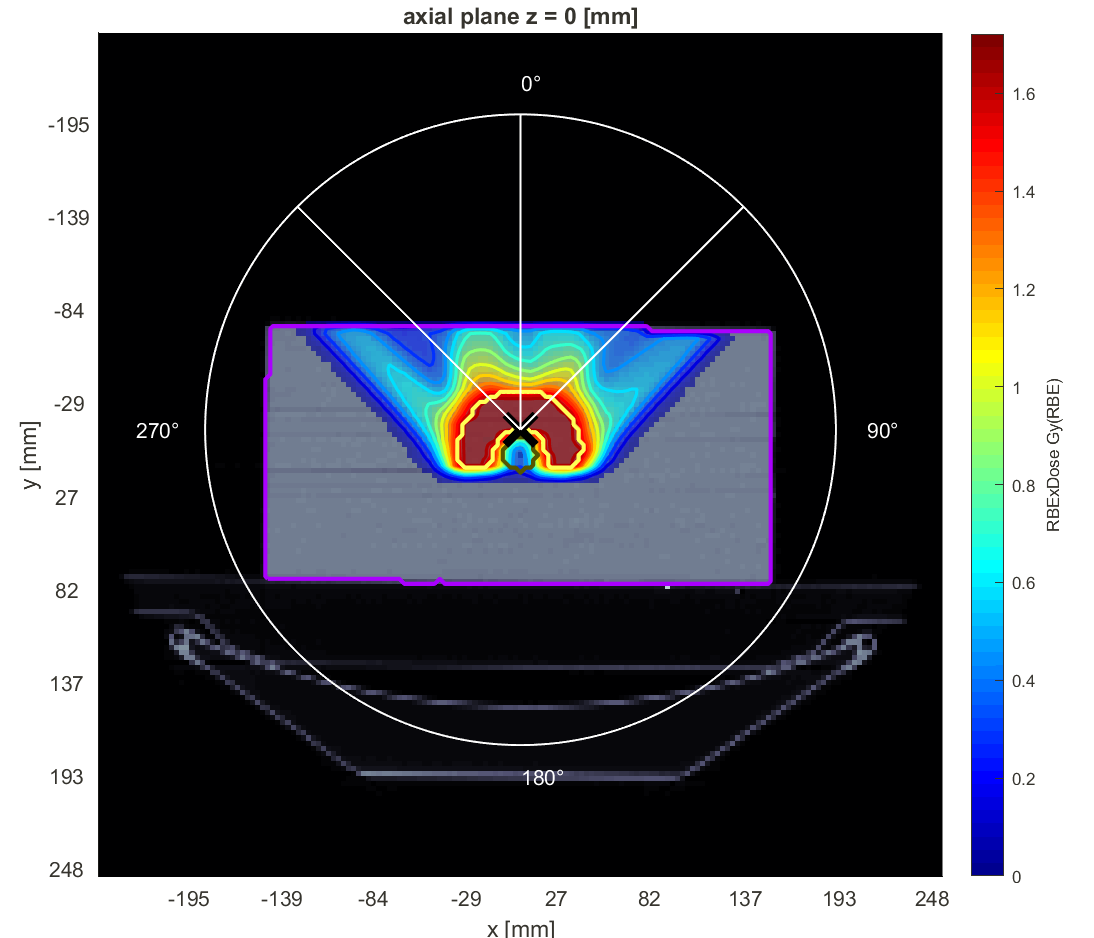
\includegraphics[width=0.6\textwidth]{images/protons/protons_3_noeq_intensity.png}
                    \caption{Protoni}
                    \label{fig:sub_protoni_3_no}
                \end{figure}
                \begin{figure}[H]
                    \centering
                    \begin{subfigure}{0.5\textwidth}
                        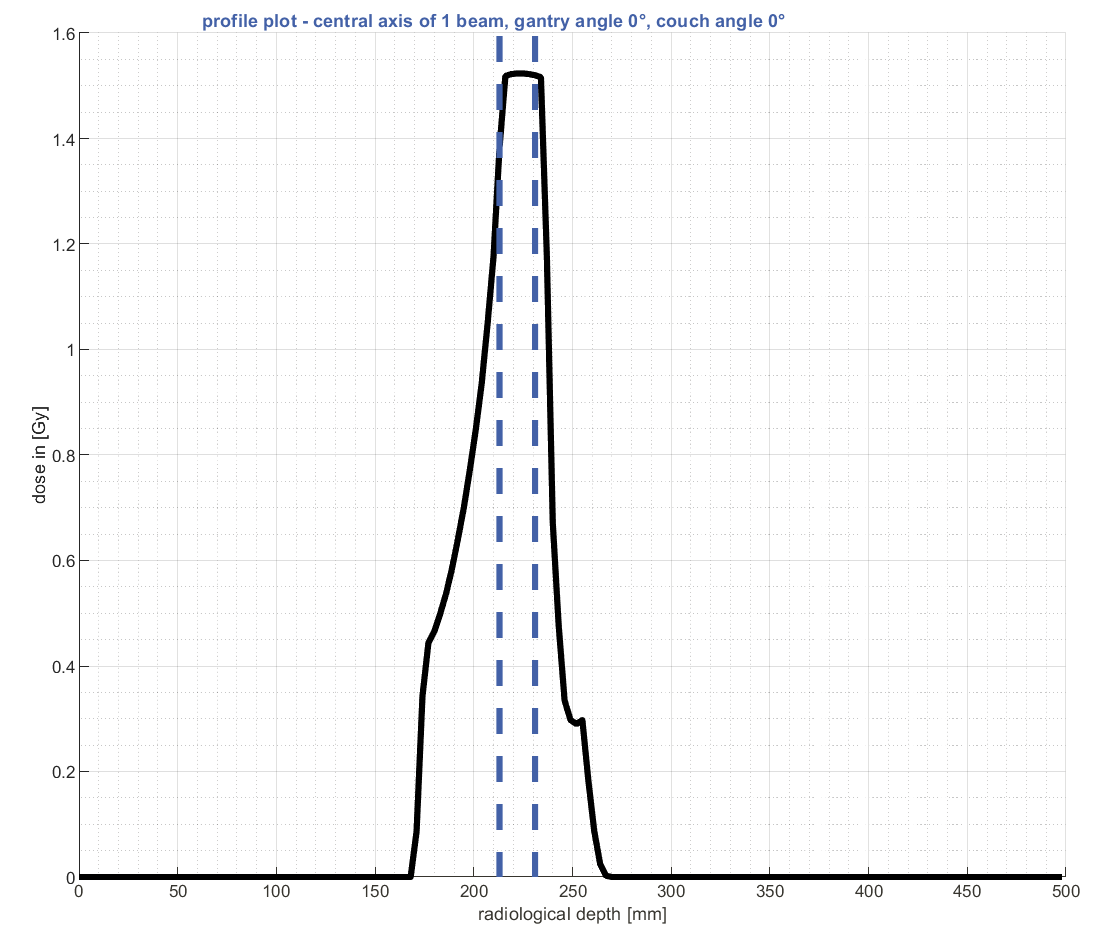
\includegraphics[width=\textwidth]{images/protons/protons_3_noeq_depth.png}
                        \caption{Profilo depth}
                        \label{fig:sub_protoni_3_no_profile_depth}
                    \end{subfigure}\hfill
                    \begin{subfigure}{0.5\textwidth}
                        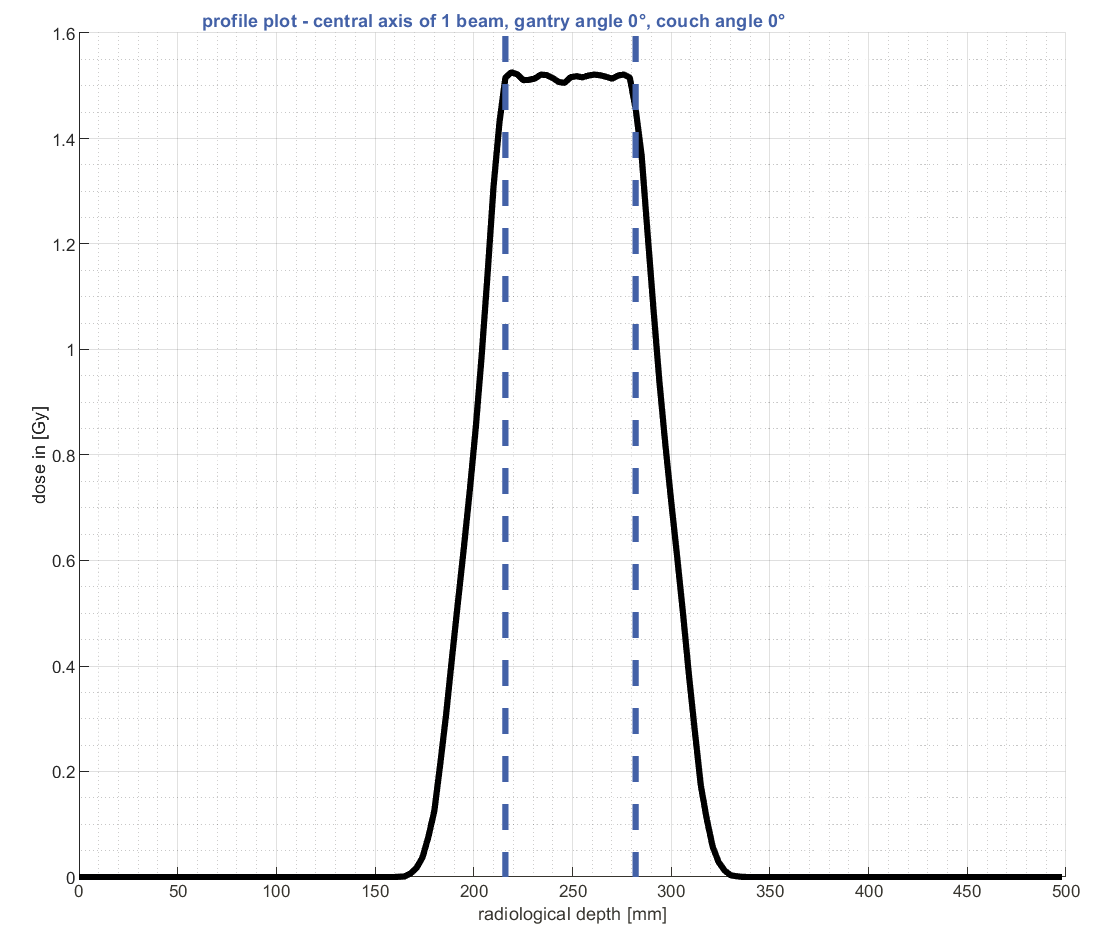
\includegraphics[width=\textwidth]{images/protons/protons_3_noeq_lateral.png}
                        \caption{Profilo lateral}
                        \label{fig:sub_protoni_3_no_profile_lateral}
                    \end{subfigure}\hfill
                    \caption{Profili del fascio di protoni}
                    \label{fig:protoni_3_no_profiles}
                \end{figure}
                \begin{figure}[H]
                    \centering
                    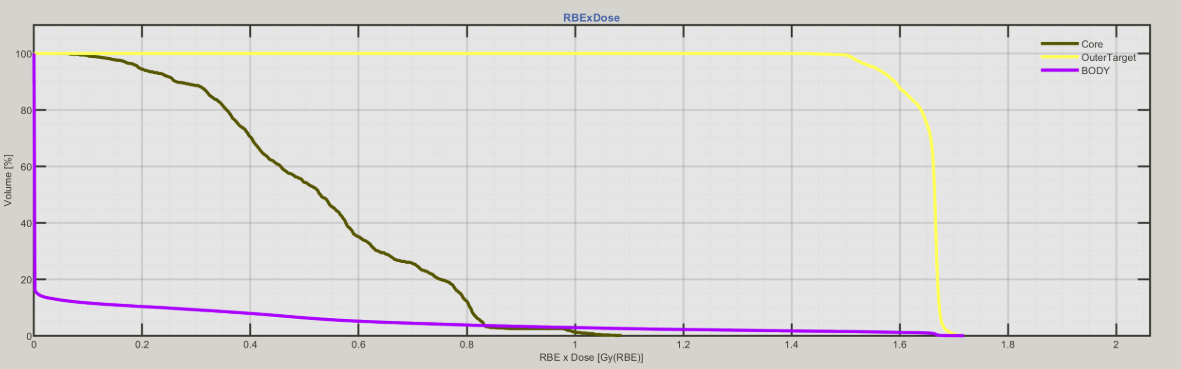
\includegraphics[width=0.6\textwidth]{images/protons/protons_3_noeq_DVH_graph.png}
                    \caption{Grafico DVH}
                    \label{fig:protoni_3_no_DVH_graph}
                \end{figure}
                \begin{table}[H]
                    \centering
                    \label{tab:dati_terza_misura_protoni}
                    \begin{tabular}{
                        l | c | c | c | c | c |
                    }
                    \toprule
                    & Mean & Std & Max & Min & D$_{98}$ \\
                    \midrule
                    Core & 0.5321 & 0.2052 & 1.0866 & 0.0389 & 0.1428 \\
                    Outer target & 1.6488 & 0.0399 & 1.7192 & 1.4143 & 1.5162 \\
                    Body & 0.0825 & 0.2769 & 1.7192 & 0 & 0 \\
                    \bottomrule
                    \end{tabular}
                    \caption{Dati ottenuti dalle curve di isodose (unità di misura della tabella [\unit{\gray}])}
                \end{table}

            \subsubsection{Ioni carbonio}
                \begin{figure}[H]
                    \centering
                    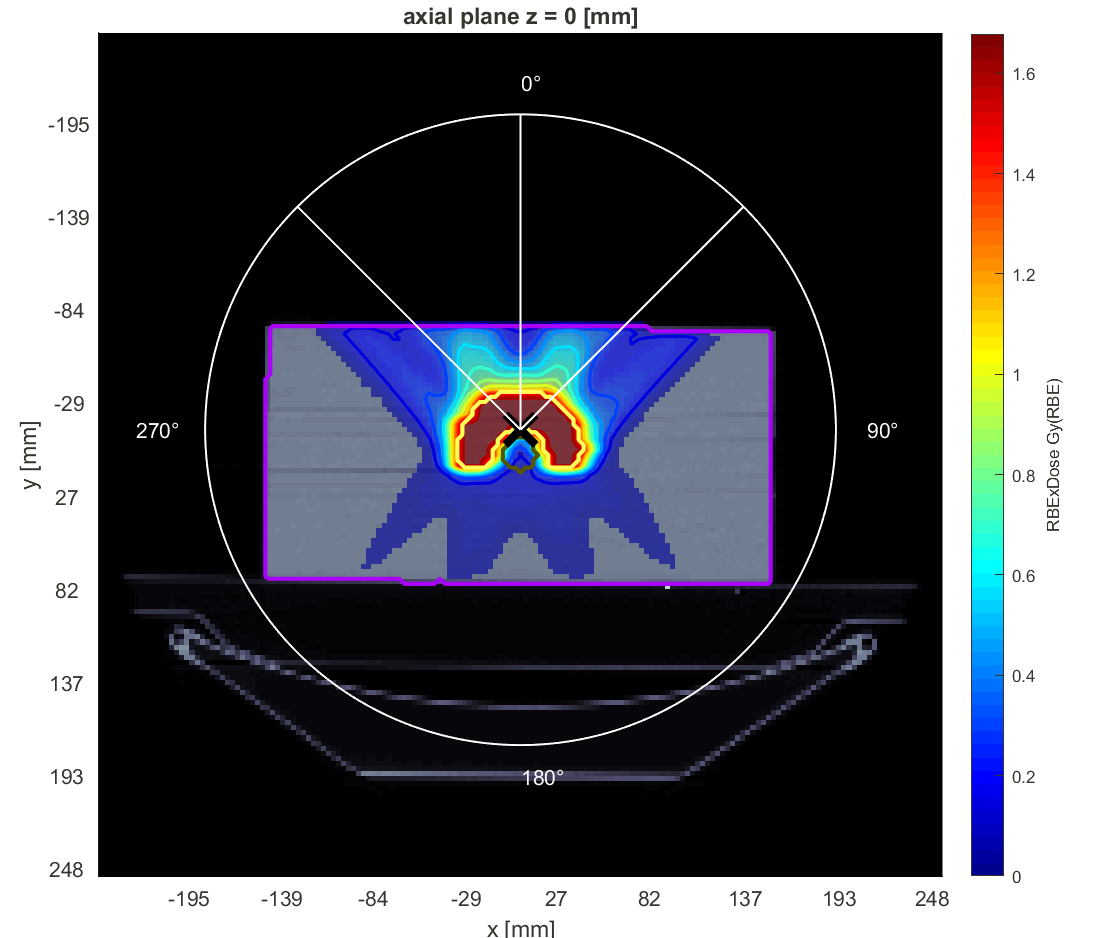
\includegraphics[width=0.6\textwidth]{images/carbon/carbon_3_noeq_intensity.png}
                    \caption{Ioni carbonio}
                    \label{fig:carbonio_3_no}
                \end{figure}
                \begin{figure}[H]
                    \centering
                    \begin{subfigure}{0.5\textwidth}
                        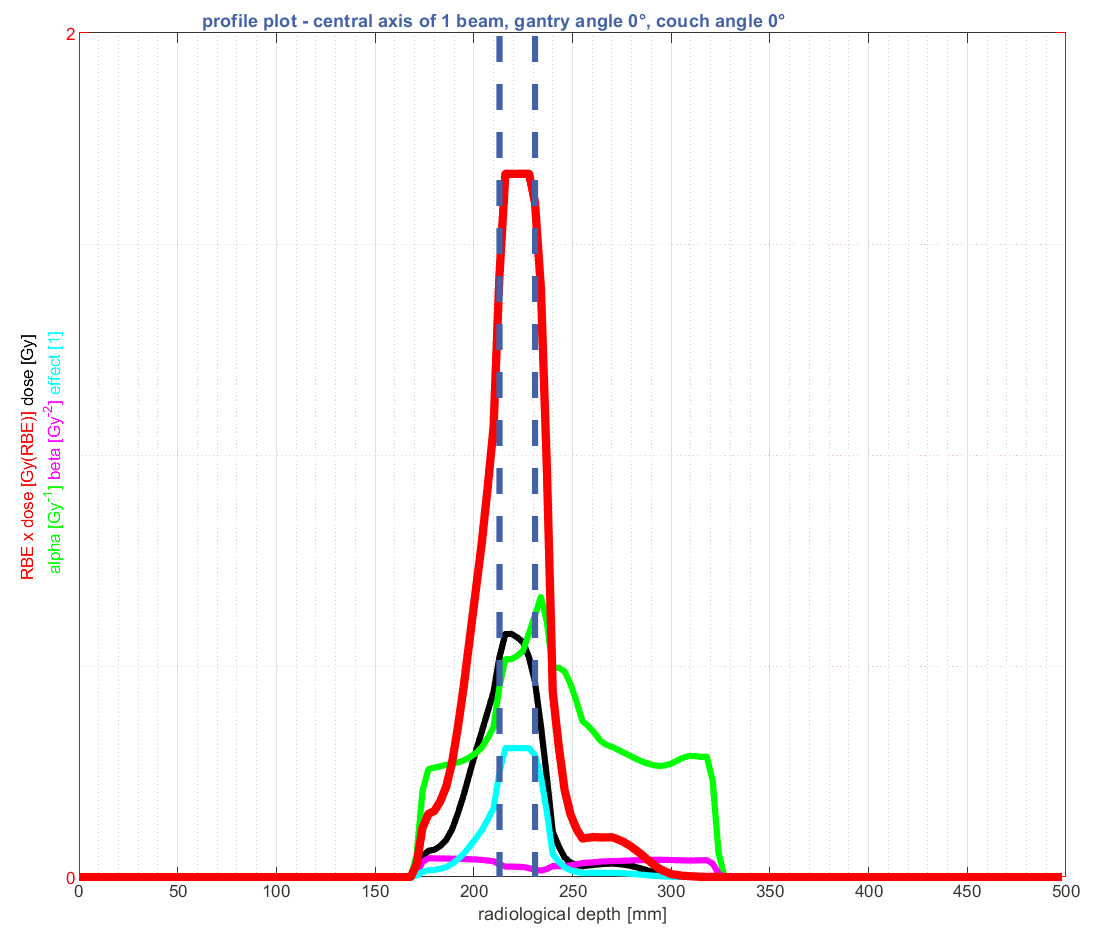
\includegraphics[width=\textwidth]{images/carbon/carbon_3_noeq_depth.png}
                        \caption{Profilo depth}
                        \label{fig:sub_carbonio_3_no_profile_depth}
                    \end{subfigure}\hfill
                    \begin{subfigure}{0.5\textwidth}
                        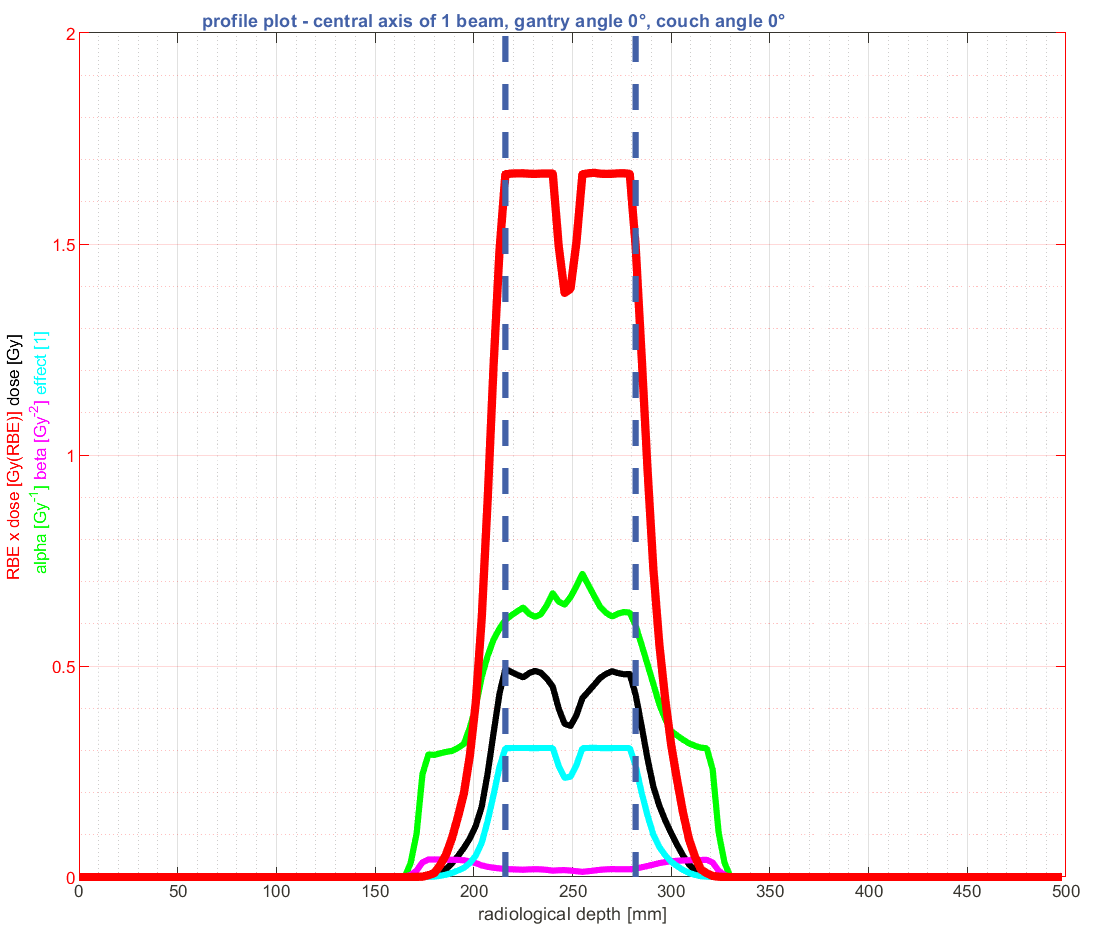
\includegraphics[width=\textwidth]{images/carbon/carbon_3_noeq_lateral.png}
                        \caption{Profilo lateral}
                        \label{fig:sub_carbonio_3_no_profile_lateral}
                    \end{subfigure}\hfill
                    \caption{Profili del fascio di ioni carbonio}
                    \label{fig:carbonio_3_no_profiles}
                \end{figure}
                \begin{figure}[H]
                    \centering
                    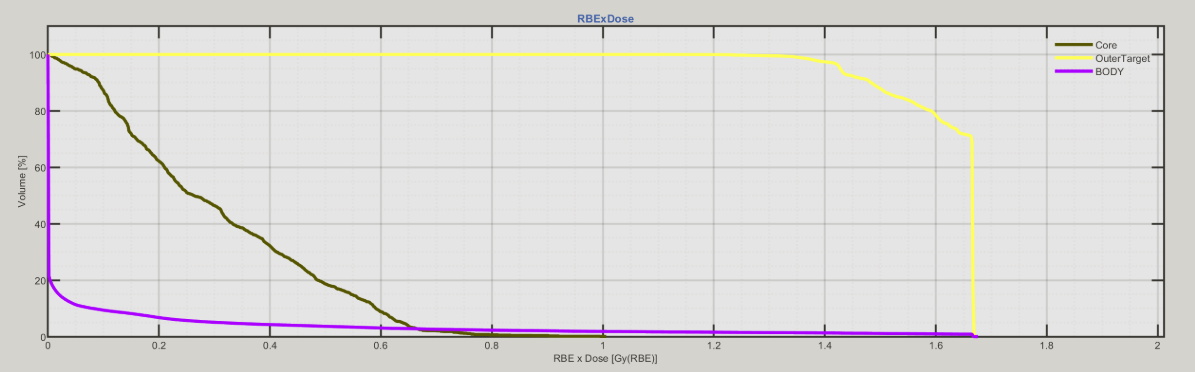
\includegraphics[width=0.6\textwidth]{images/carbon/carbon_3_noeq_DVH_graph.png}
                    \caption{Grafico DVH}
                    \label{fig:carbon_3_no_DVH_graph}
                \end{figure}
                \begin{table}[H]
                    \centering
                    \label{tab:dati_terza_misura_carbonio}
                    \begin{tabular}{
                        l | c | c | c | c | c |
                    }
                    \toprule
                    & Mean & Std & Max & Min & D$_{98}$ \\
                    \midrule
                    Core & 0.3058 & 0.1933 & 1.0074 & 0.0048 & 0.0208 \\
                    Outer target & 1.6241 & 0.0829 & 1.6765 & 1.1136 & 1.3803 \\
                    Body & 0.0570 & 0.2281 & 1.6765 & 0 & 0 \\
                    \bottomrule
                    \end{tabular}
                    \caption{Dati ottenuti dalle curve di isodose (unità di misura della tabella [\unit{\gray}])}
                \end{table}     

        \subsection{4 fasci equidistanziati}
            \subsubsection{Fotoni}
                \begin{figure}[H]
                    \centering
                    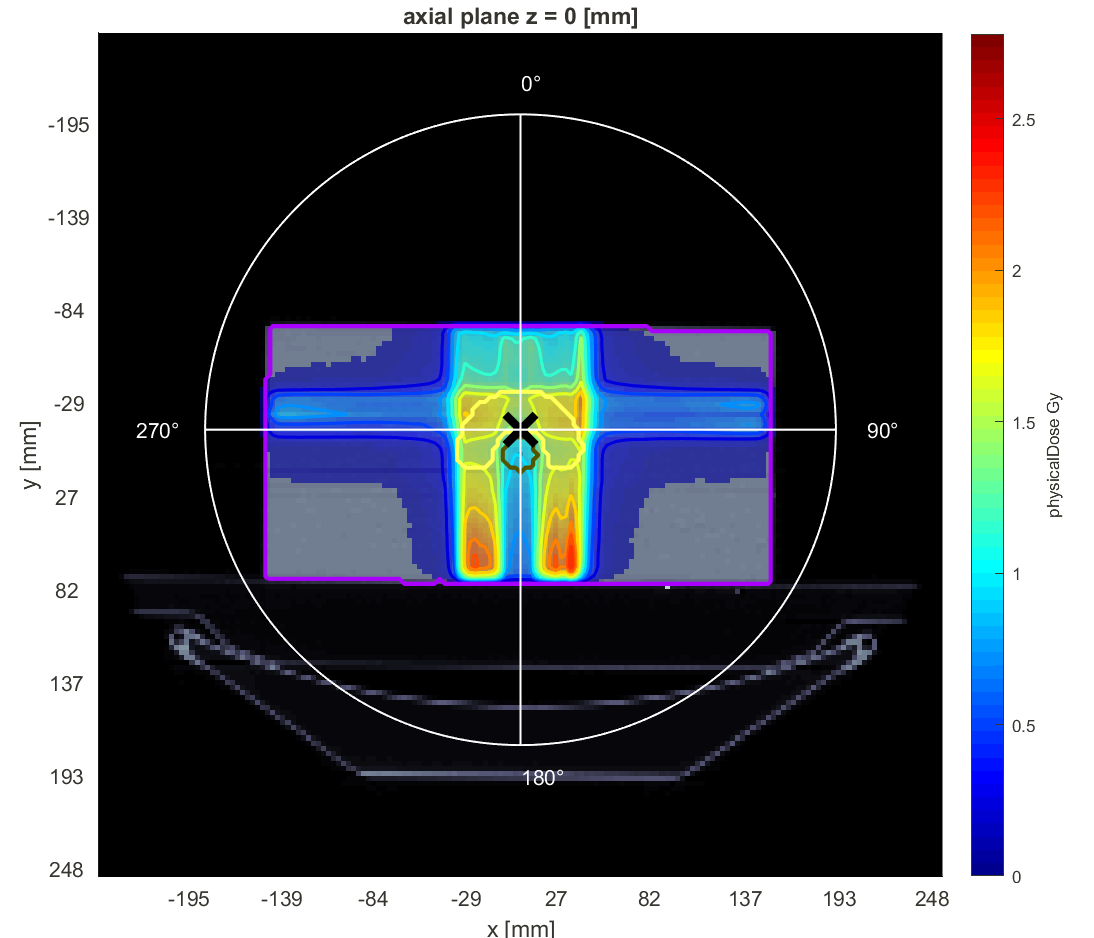
\includegraphics[width=0.6\textwidth]{images/photons/photons_4_eq_intensity.png}
                    \caption{Intensità fasci fotoni}
                    \label{fig:sub_fotoni_4}
                \end{figure}
                \begin{figure}[H]
                    \centering
                    \begin{subfigure}{0.5\textwidth}
                        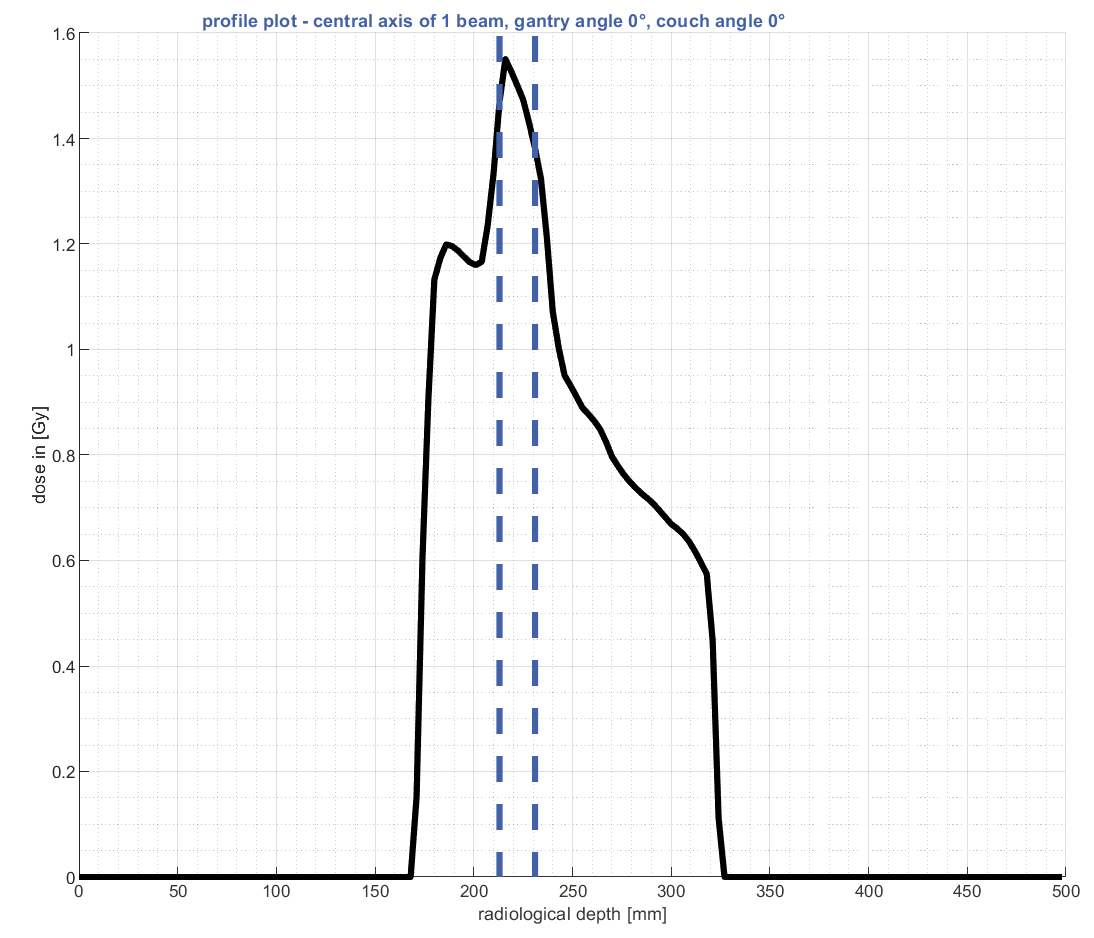
\includegraphics[width=\textwidth]{images/photons/photons_4_eq_depth.png}
                        \caption{Profilo depth}
                        \label{fig:sub_fotoni_4_profile_depth}
                    \end{subfigure}\hfill
                    \begin{subfigure}{0.5\textwidth}
                        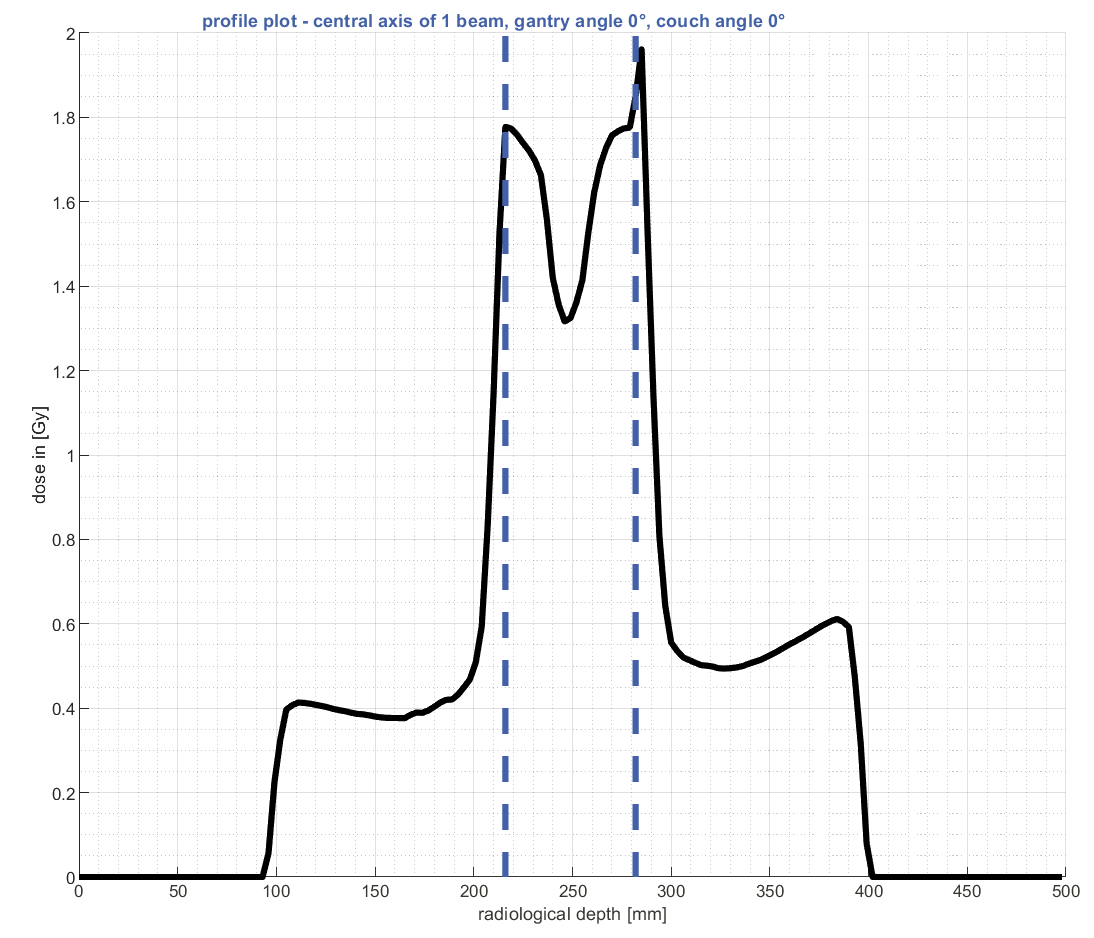
\includegraphics[width=\textwidth]{images/photons/photons_4_eq_lateral.png}
                        \caption{Profilo lateral}
                        \label{fig:sub_fotoni_4_profile_lateral}
                    \end{subfigure}\hfill
                    \caption{Profili dei 4 fasci di fotoni}
                    \label{fig:fotoni_4_profiles}
                \end{figure}
                \begin{figure}[H]
                    \centering
                    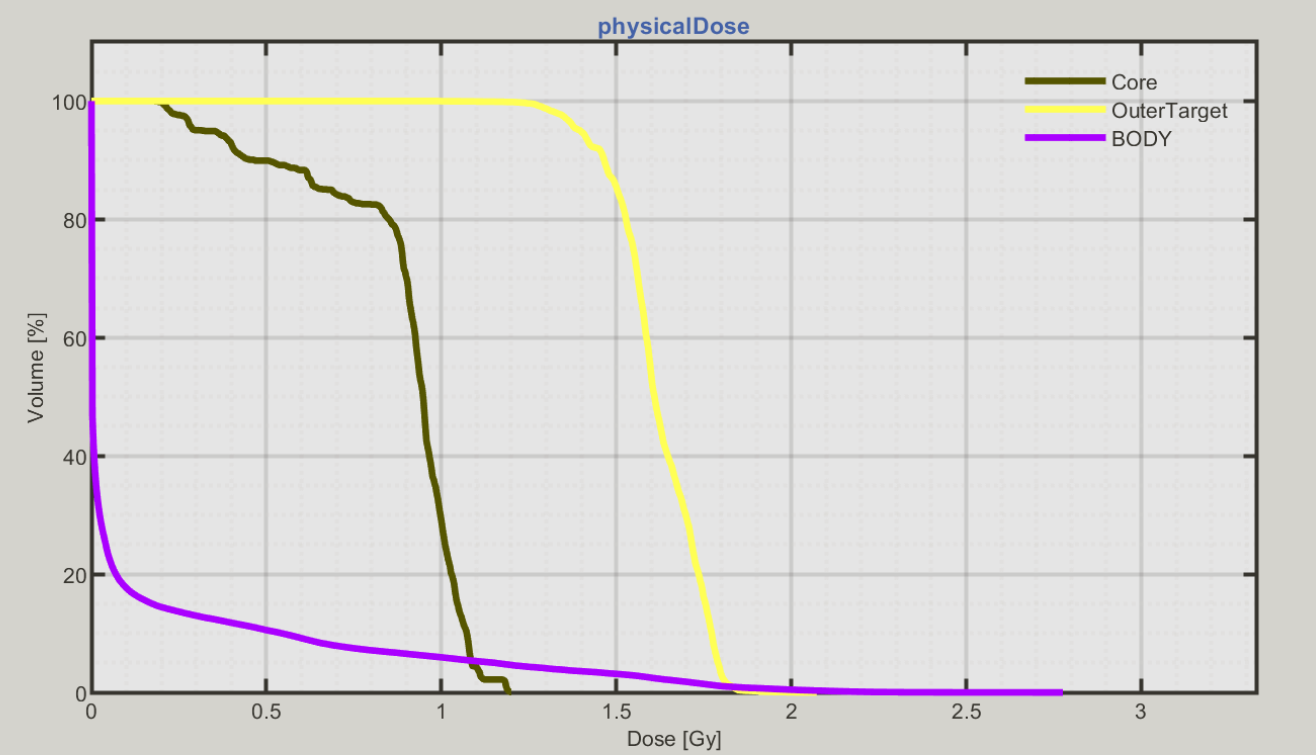
\includegraphics[width=0.6\textwidth]{images/photons/photons_4_eq_DVH_graph.png}
                    \caption{Grafico DVH}
                    \label{fig:fotoni_4_DVH_graph}
                \end{figure}
                \begin{table}[H]
                    \centering
                    \label{tab:dati_seconda_misura_fotoni}
                    \begin{tabular}{
                        l | c | c | c | c | c |
                    }
                    \toprule
                    & Mean & Std & Max & Min & D$_{98}$ \\
                    \midrule
                    Core & 0.8852 & 0.2197 & 1.2018 & 0.1823 & 0.2304 \\
                    Outer target & 1.6167 & 0.1219 & 2.0730 & 0.9925 & 1.3287 \\
                    Body & 0.1484 & 0.3877 & 2.7772 & 0 & 0 \\
                    \bottomrule
                    \end{tabular}
                    \caption{Dati ottenuti dalle curve di isodose (unità di misura della tabella [\unit{\gray}])}
                \end{table}

            \subsubsection{Protoni}
                \begin{figure}[H]
                    \centering
                    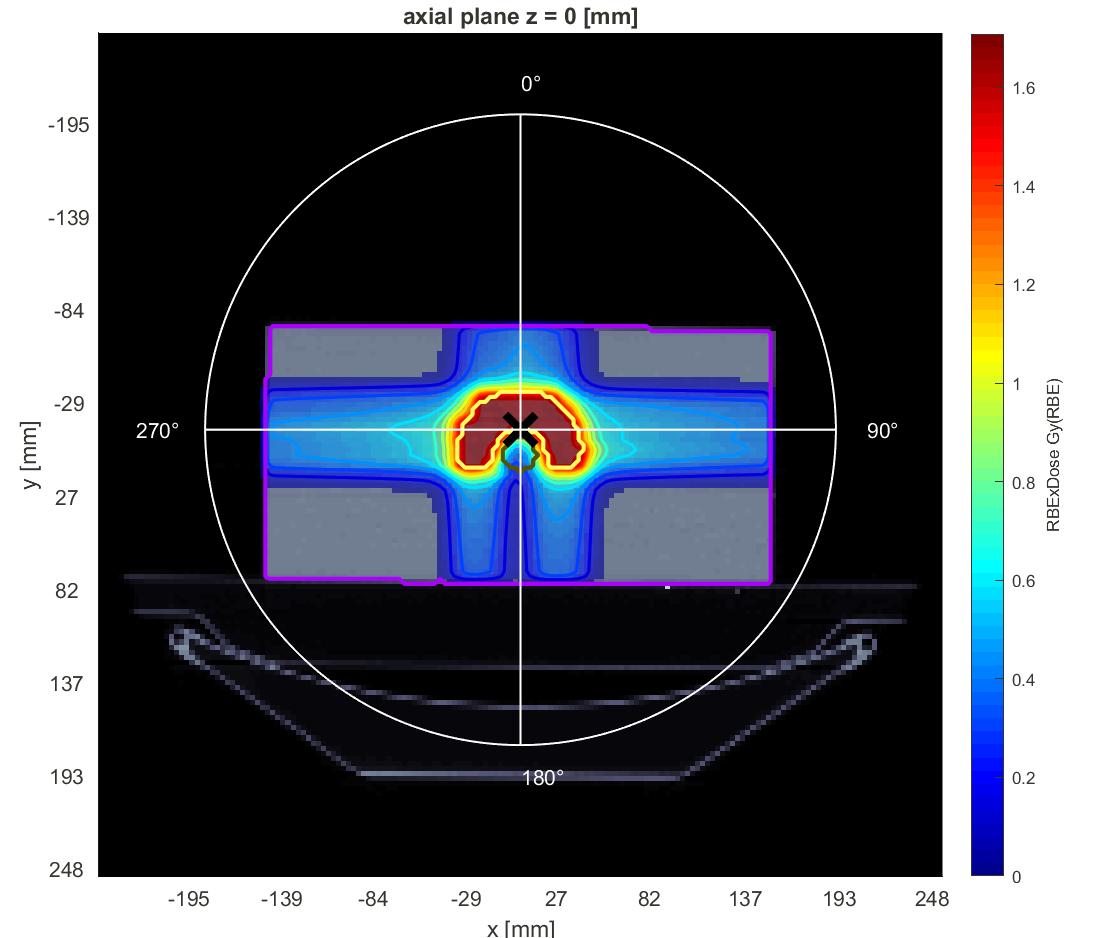
\includegraphics[width=0.6\textwidth]{images/protons/protons_4_eq_intensity.png}
                    \caption{Intensità fasci protoni}
                    \label{fig:sub_protoni_4}
                \end{figure}
                \begin{figure}[H]
                    \centering
                    \begin{subfigure}{0.5\textwidth}
                        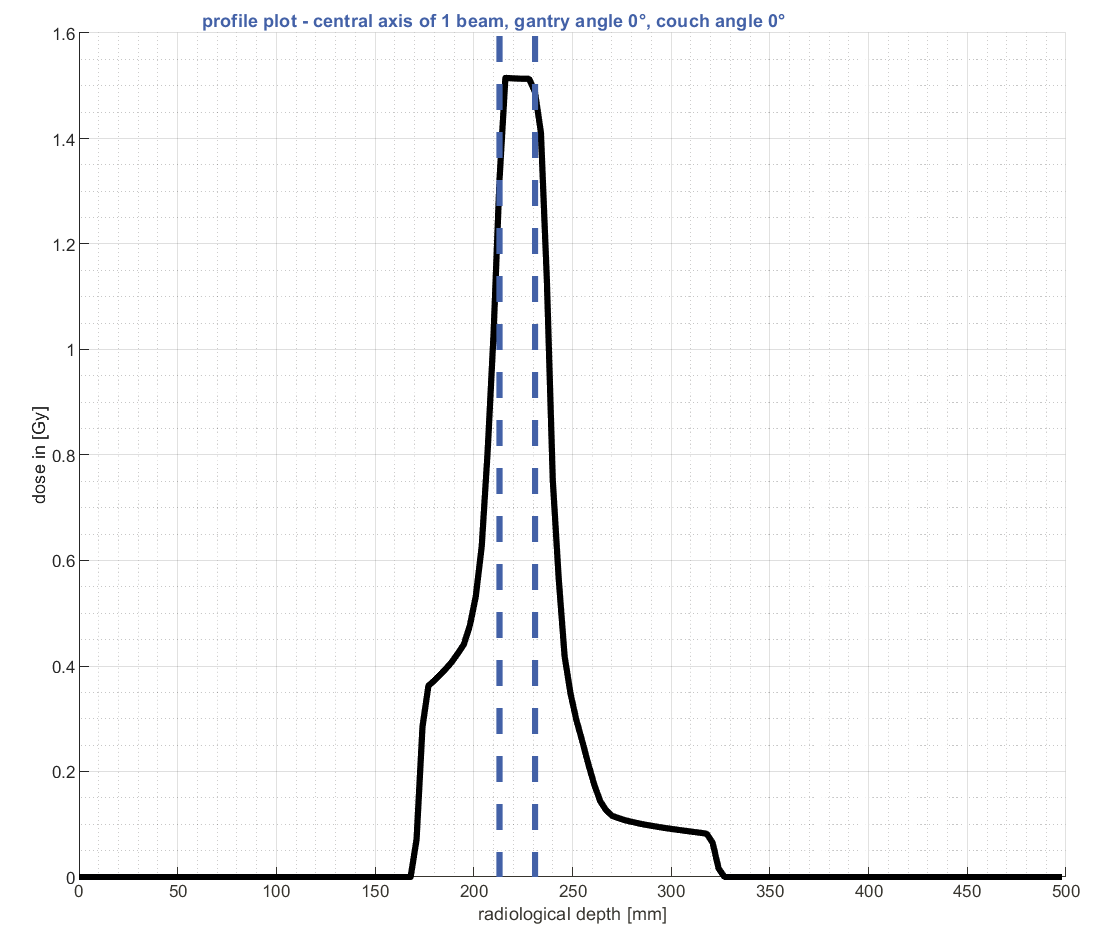
\includegraphics[width=\textwidth]{images/protons/protons_4_eq_depth.png}
                        \caption{Profilo depth}
                        \label{fig:sub_protoni_4_profile_depth}
                    \end{subfigure}\hfill
                    \begin{subfigure}{0.5\textwidth}
                        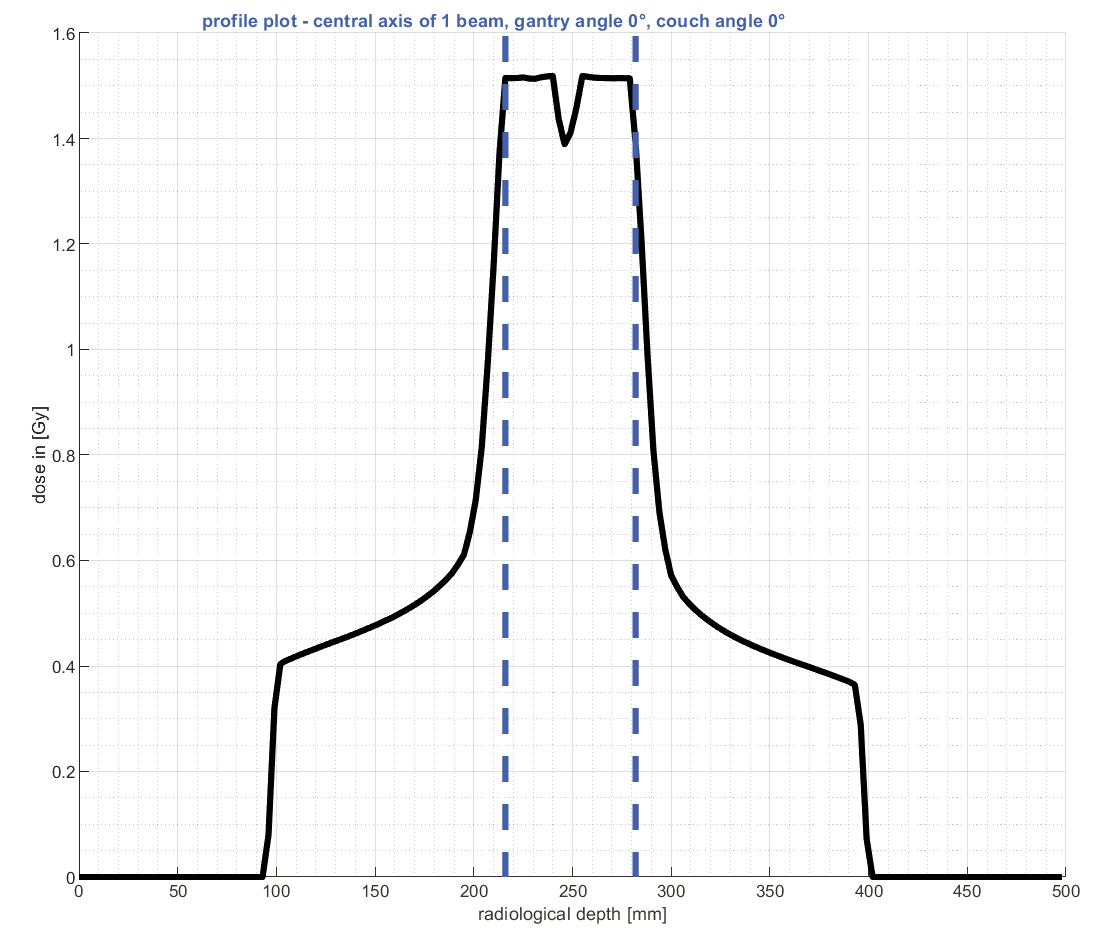
\includegraphics[width=\textwidth]{images/protons/protons_4_eq_lateral.png}
                        \caption{Profilo lateral}
                        \label{fig:sub_protoni_4_profile_lateral}
                    \end{subfigure}\hfill
                    \caption{Profili dei 4 fasci di protoni}
                    \label{fig:protoni_4_profiles}
                \end{figure}
                \begin{figure}[H]
                    \centering
                    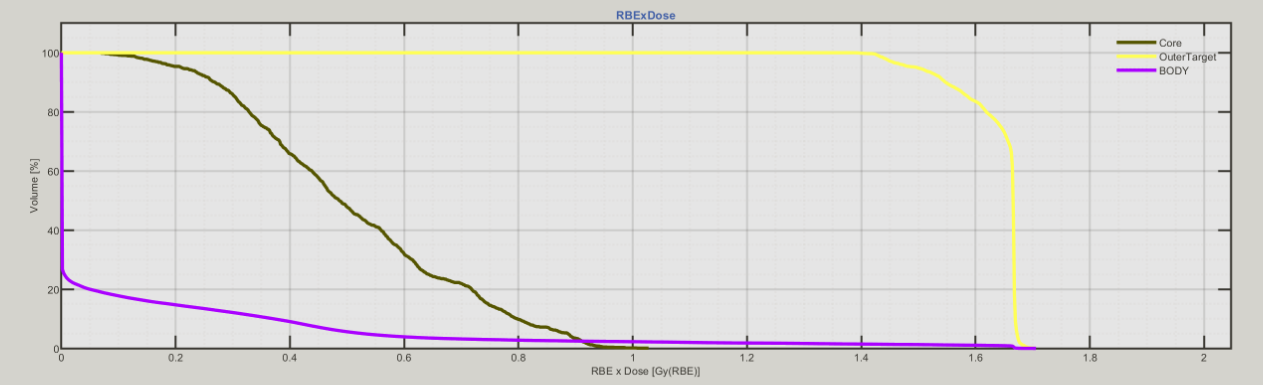
\includegraphics[width=0.6\textwidth]{images/protons/protons_4_eq_DVH_graph.png}
                    \caption{Grafico DVH}
                    \label{fig:protoni_4_DVH_graph}
                \end{figure}
                \begin{table}[H]
                    \centering
                    \label{tab:dati_seconda_misura_protoni}
                    \begin{tabular}{
                        l | c | c | c | c | c |
                    }
                    \toprule
                    & Mean & Std & Max & Min & D$_{98}$ \\
                    \midrule
                    Core & 0.5112 & 0.2019 & 1.0286 & 0.0683 & 0.1431 \\
                    Outer target & 1.6388 & 0.0580 & 1.7064 & 1.3871 & 1.4424 \\
                    Body & 0.0945 & 0.2613 & 1.7064 & 0 & 0 \\
                    \bottomrule
                    \end{tabular}
                    \caption{Dati ottenuti dalle curve di isodose (unità di misura della tabella [\unit{\gray}])}
                \end{table}

            \subsubsection{Ioni carbonio}
                \begin{figure}[H]
                    \centering
                    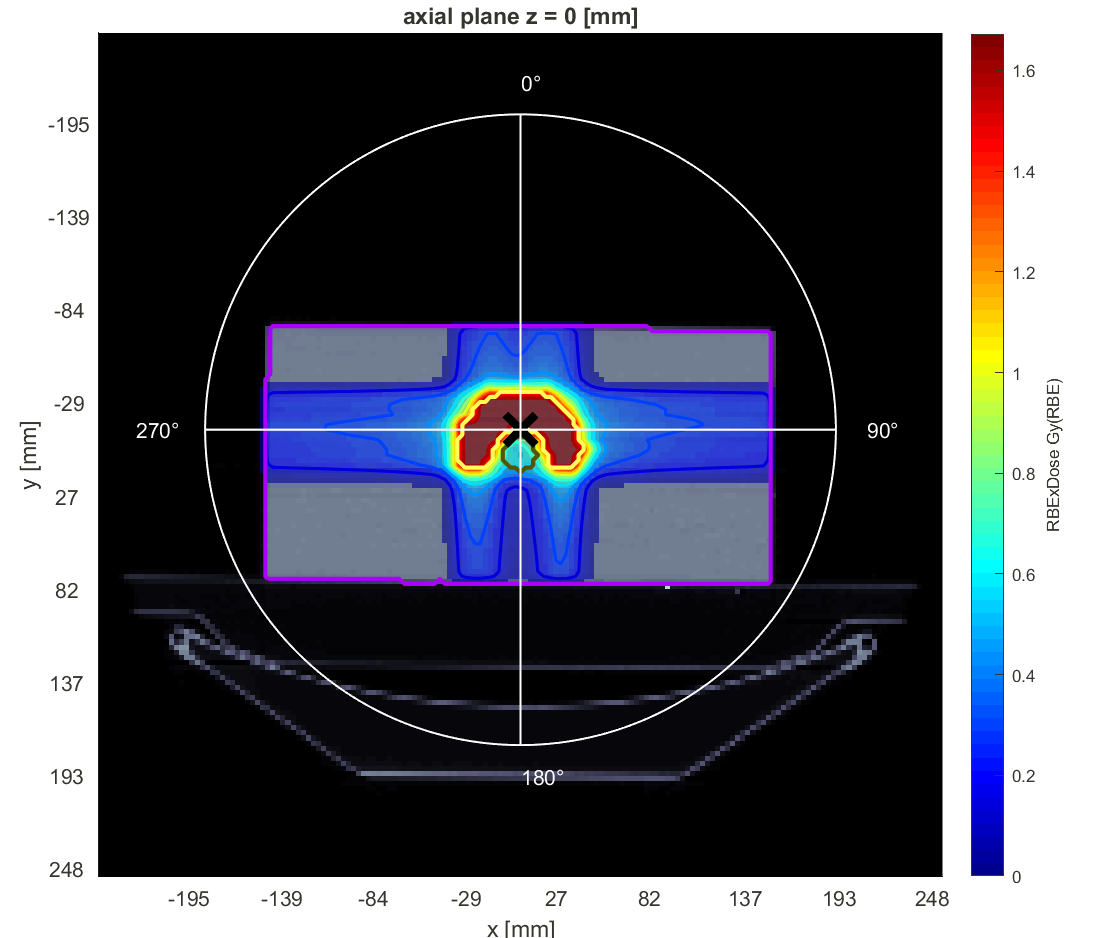
\includegraphics[width=0.6\textwidth]{images/carbon/carbon_4_eq_intensity.png}
                    \caption{Intensità ioni carbonio}
                    \label{fig:sub_carbonio_4}
                \end{figure}
                \begin{figure}[H]
                    \centering
                    \begin{subfigure}{0.5\textwidth}
                        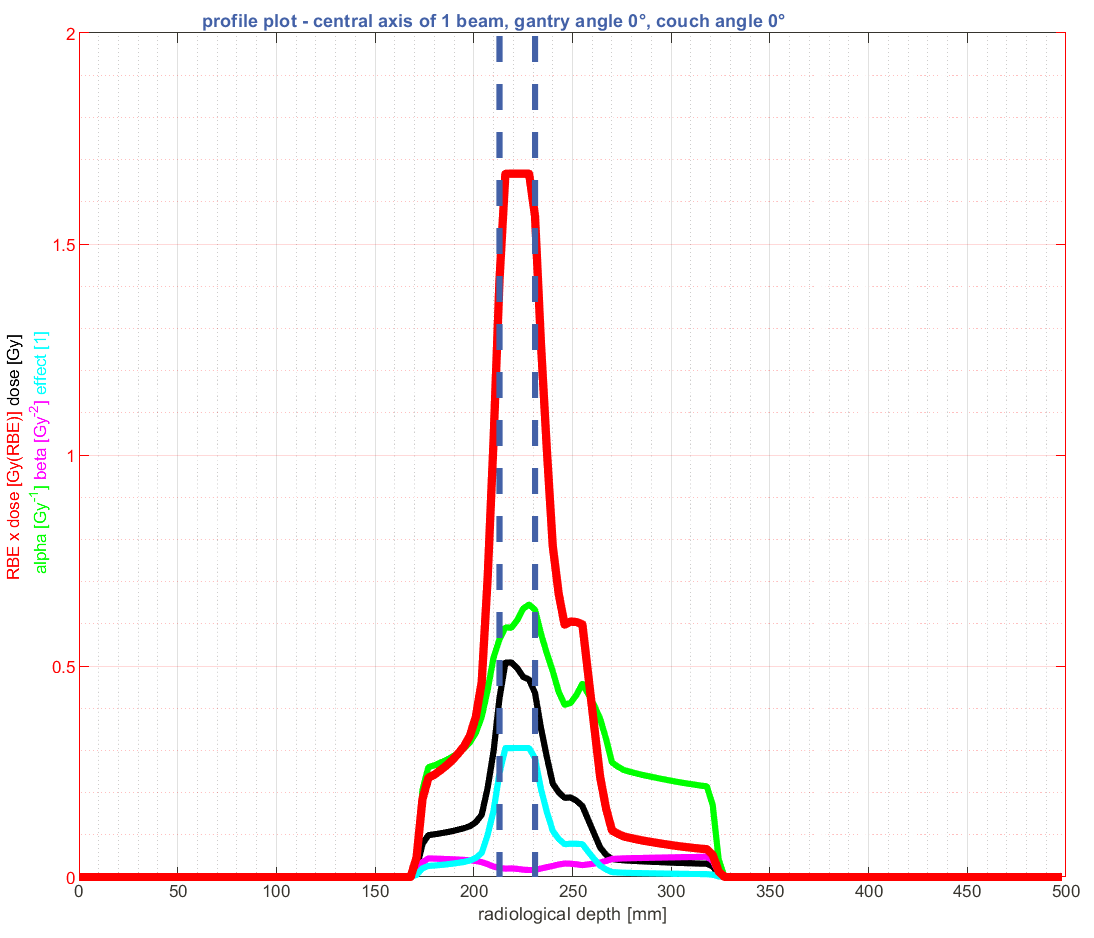
\includegraphics[width=\textwidth]{images/carbon/carbon_4_eq_depth.png}
                        \caption{Profilo depth}
                        \label{fig:sub_carbonio_4_profile_depth}
                    \end{subfigure}\hfill
                    \begin{subfigure}{0.5\textwidth}
                        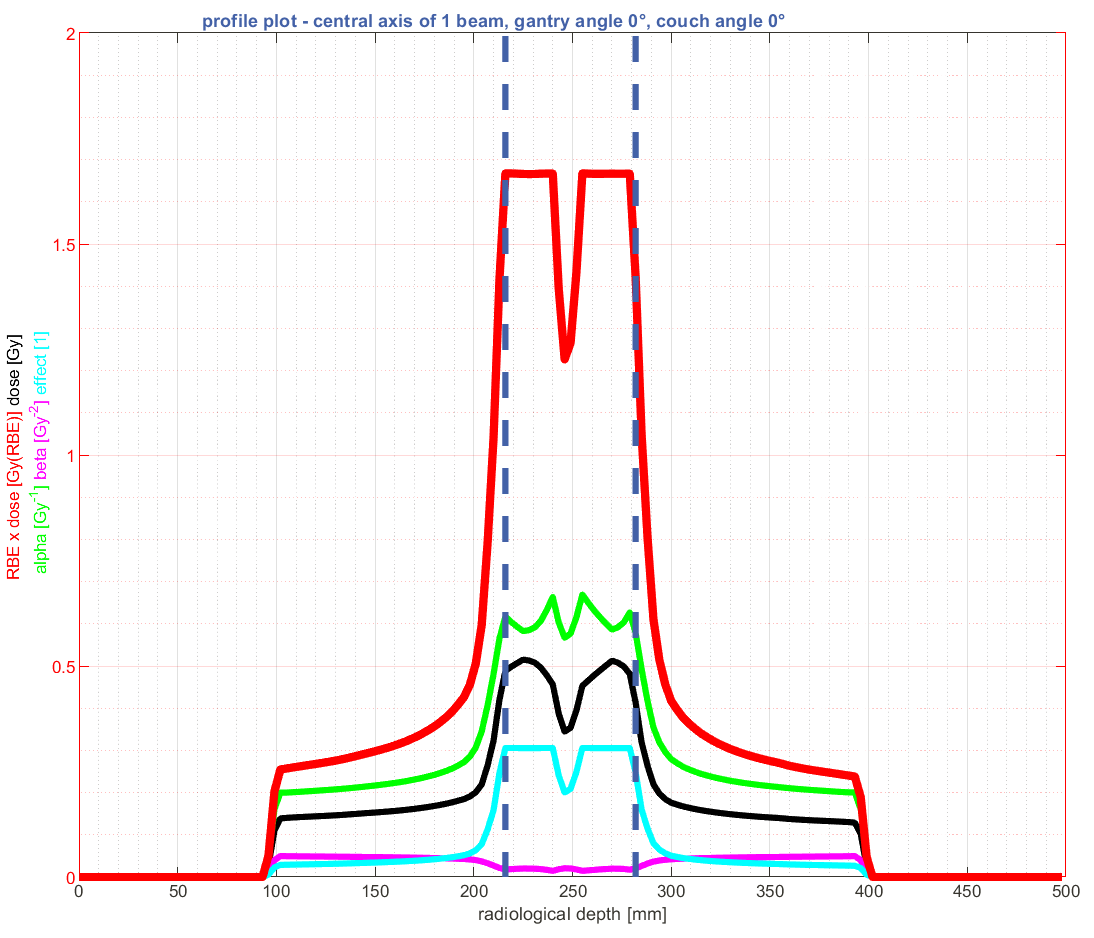
\includegraphics[width=\textwidth]{images/carbon/carbon_4_eq_lateral.png}
                        \caption{Profilo lateral}
                        \label{fig:sub_carbonio_4_profile_lateral}
                    \end{subfigure}\hfill
                    \caption{Profili dei 4 fasci di ioni carbonio}
                    \label{fig:carbonio_4_profiles}
                \end{figure}
                \begin{figure}[H]
                    \centering
                    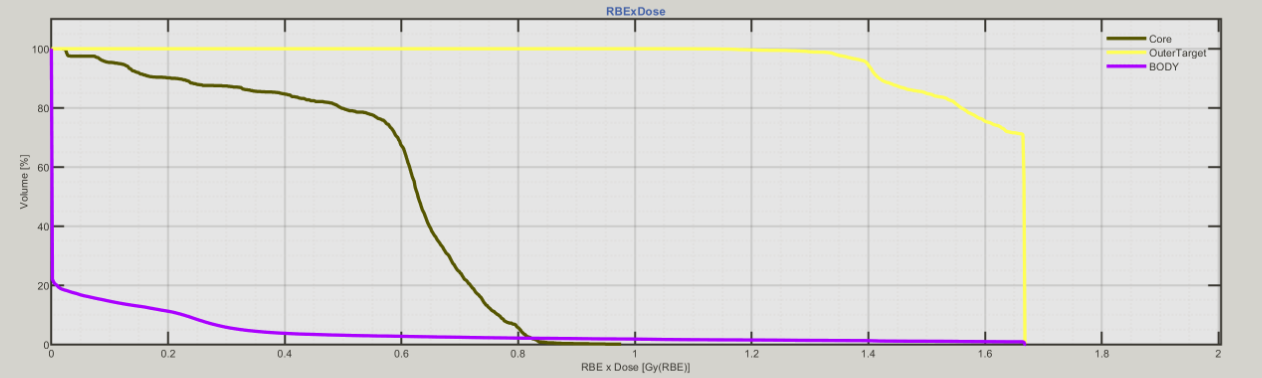
\includegraphics[width=0.6\textwidth]{images/carbon/carbon_4_eq_DVH_graph.png}
                    \caption{Grafico DVH}
                    \label{fig:carbon_4_DVH_graph}
                \end{figure}
                \begin{table}[H]
                    \centering
                    \label{tab:dati_seconda_misura_carbonio}
                    \begin{tabular}{
                        l | c | c | c | c | c |
                    }
                    \toprule
                    & Mean & Std & Max & Min & D$_{98}$ \\
                    \midrule
                    Core & 0.5803 & 0.1975 & 0.9769 & 0.0192 & 0.0273 \\
                    Outer target & 1.6143 & 0.0994 & 1.6707 & 1.0565 & 1.3452 \\
                    Body & 0.0667 & 0.2251 & 1.6707 & 0 & 0 \\
                    \bottomrule
                    \end{tabular}
                    \caption{Dati ottenuti dalle curve di isodose (unità di misura della tabella [\unit{\gray}])}
                \end{table}
           
        \subsection{4 fasci non equidistanziati}
            \subsubsection{Fotoni}
                \begin{figure}[H]
                    \centering
                    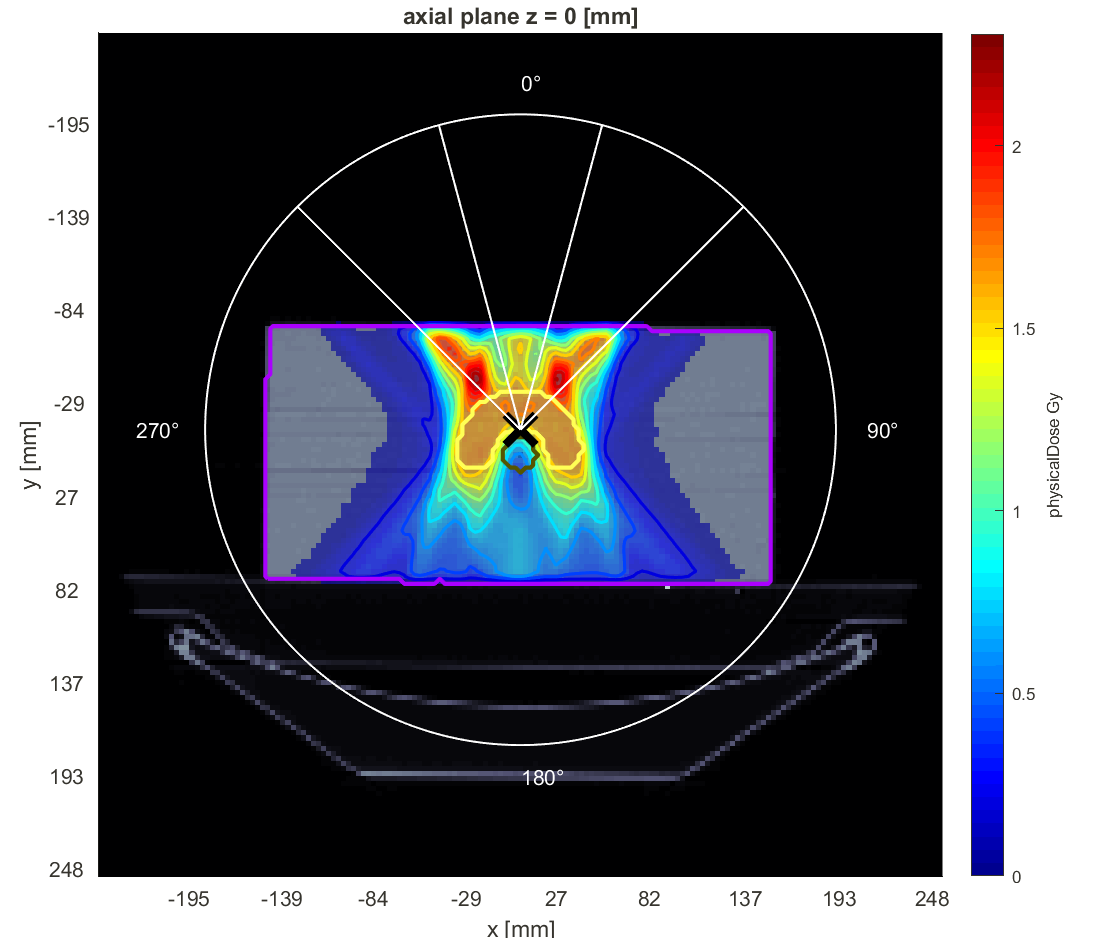
\includegraphics[width=0.6\textwidth]{images/photons/photons_4_noeq_intensity.png}
                    \caption{Fotoni}
                    \label{fig:sub_fotoni_4_no}
                \end{figure}
                \begin{figure}[H]
                    \centering
                    \begin{subfigure}{0.5\textwidth}
                        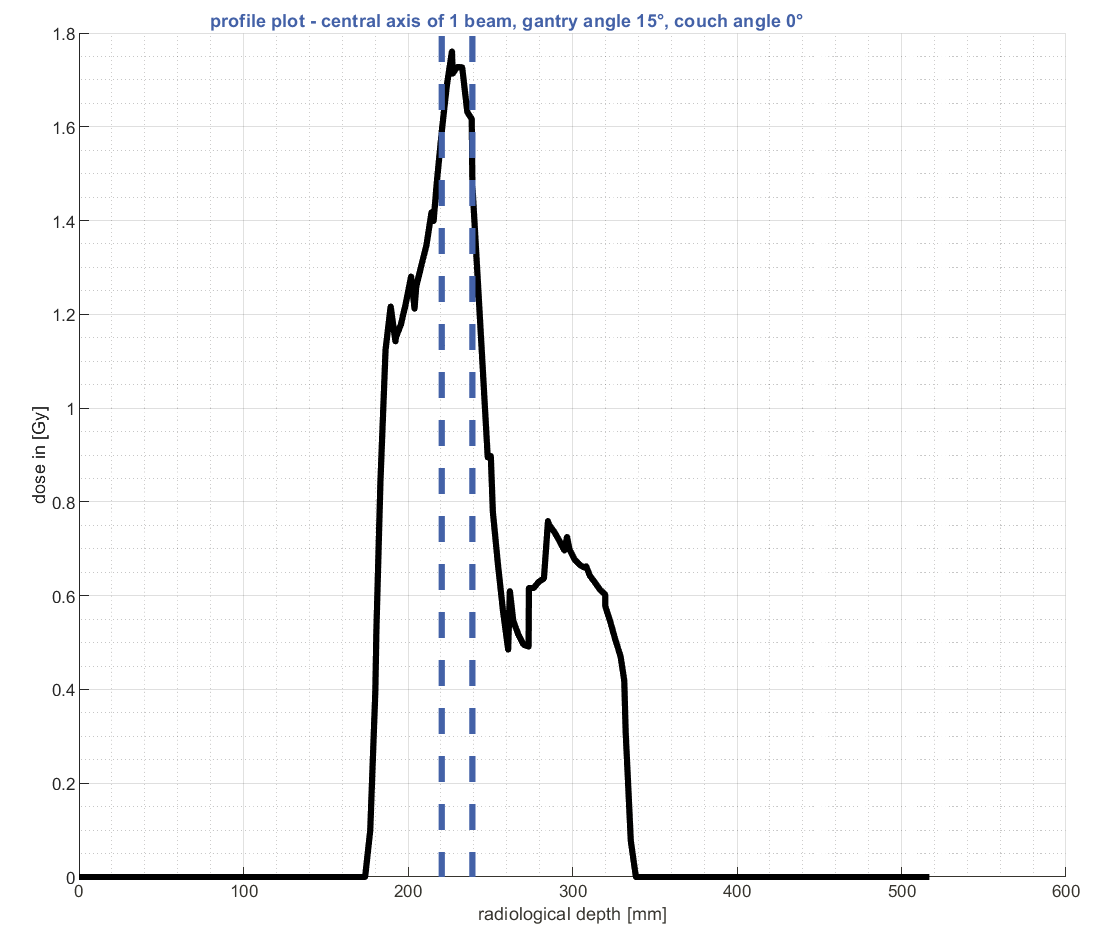
\includegraphics[width=\textwidth]{images/photons/photons_4_noeq_depth.png}
                        \caption{Profilo depth}
                        \label{fig:sub_fotoni_4_no_profile_depth}
                    \end{subfigure}\hfill
                    \begin{subfigure}{0.5\textwidth}
                        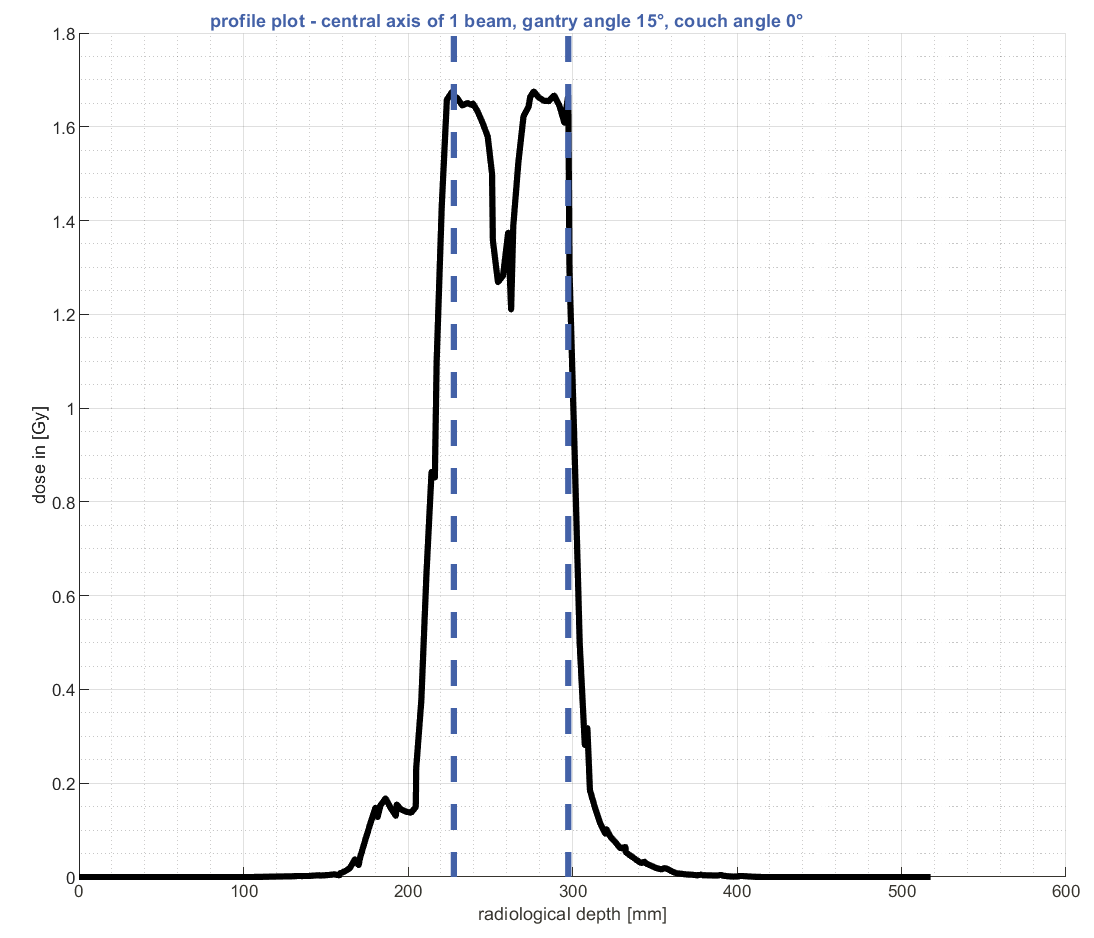
\includegraphics[width=\textwidth]{images/photons/photons_4_noeq_lateral.png}
                        \caption{Profilo lateral}
                        \label{fig:sub_fotoni_4_no_profile_lateral}
                    \end{subfigure}\hfill
                    \caption{Profili del fascio di fotoni}
                    \label{fig:fotoni_4_no_profiles}
                \end{figure}
                \begin{figure}[H]
                    \centering
                    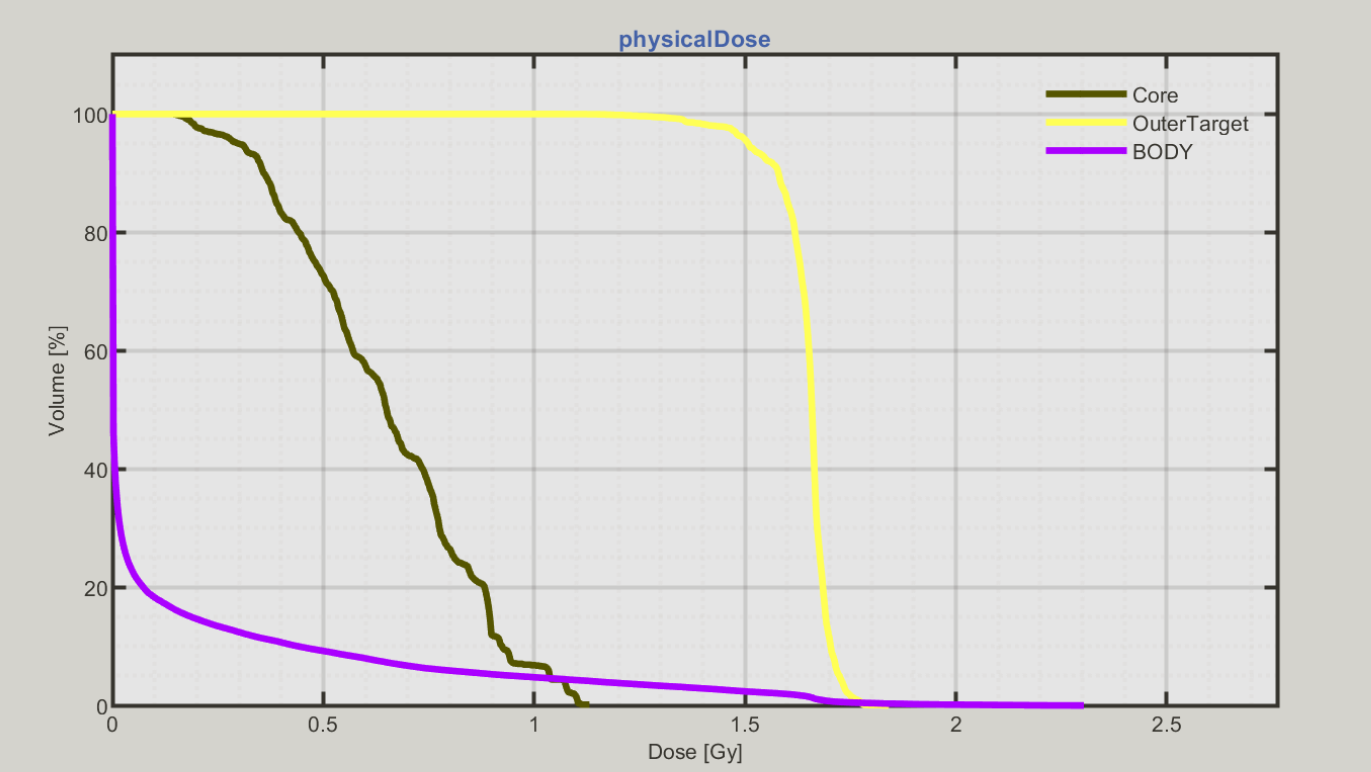
\includegraphics[width=0.6\textwidth]{images/photons/photons_4_noeq_DVH_graph.png}
                    \caption{Grafico DVH}
                    \label{fig:fotoni_4_no_DVH_graph}
                \end{figure}
                \begin{table}[H]
                    \centering
                    \label{tab:dati_terza_misura_fotoni}
                    \begin{tabular}{
                        l | c | c | c | c | c |
                    }
                    \toprule
                    & Mean & Std & Max & Min & D$_{98}$ \\
                    \midrule
                    Core & 0.6508 & 0.2239 & 1.1331 & 0.1472 & 0.1955 \\
                    Outer target & 1.6444 & 0.0694 & 1.8408 & 1.0741 & 1.4293 \\
                    Body & 0.1314 & 0.3462 & 2.3044 & 0 & 0 \\
                    \bottomrule
                    \end{tabular}
                    \caption{Dati ottenuti dalle curve di isodose (unità di misura della tabella [\unit{\gray}])}
                \end{table}

            \subsubsection{Protoni}
                \begin{figure}[H]
                    \centering
                    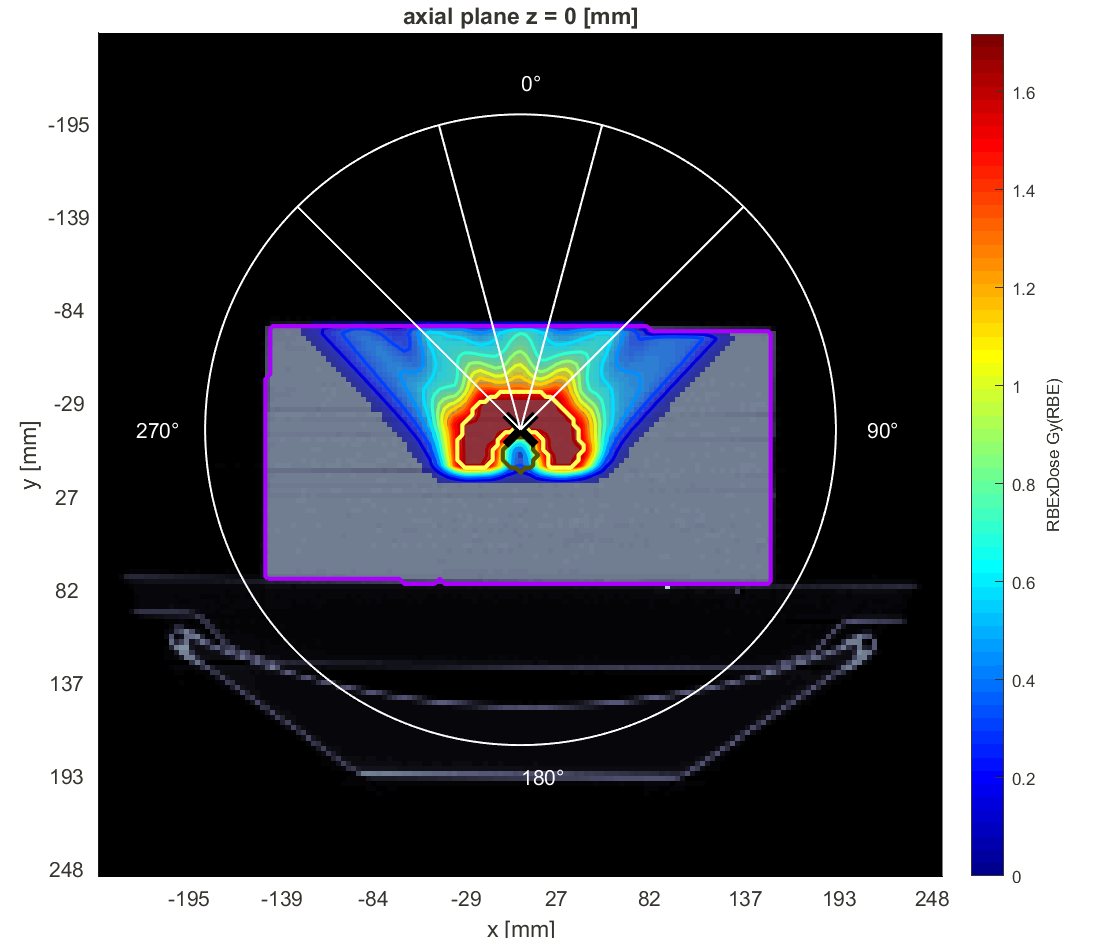
\includegraphics[width=0.6\textwidth]{images/protons/protons_4_noeq_intensity.png}
                    \caption{Protoni}
                    \label{fig:sub_protoni_4_no}
                \end{figure}
                \begin{figure}[H]
                    \centering
                    \begin{subfigure}{0.5\textwidth}
                        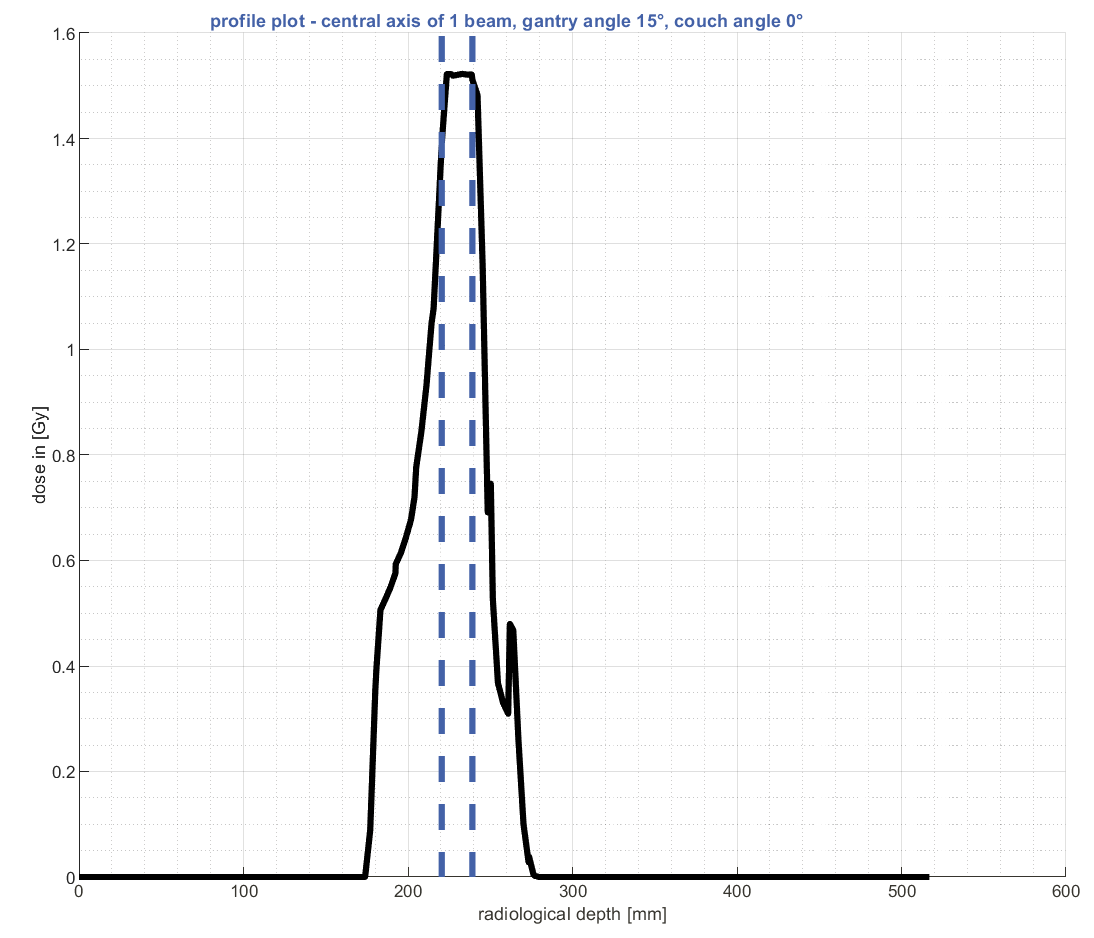
\includegraphics[width=\textwidth]{images/protons/protons_4_noeq_depth.png}
                        \caption{Profilo depth}
                        \label{fig:sub_protoni_4_no_profile_depth}
                    \end{subfigure}\hfill
                    \begin{subfigure}{0.5\textwidth}
                        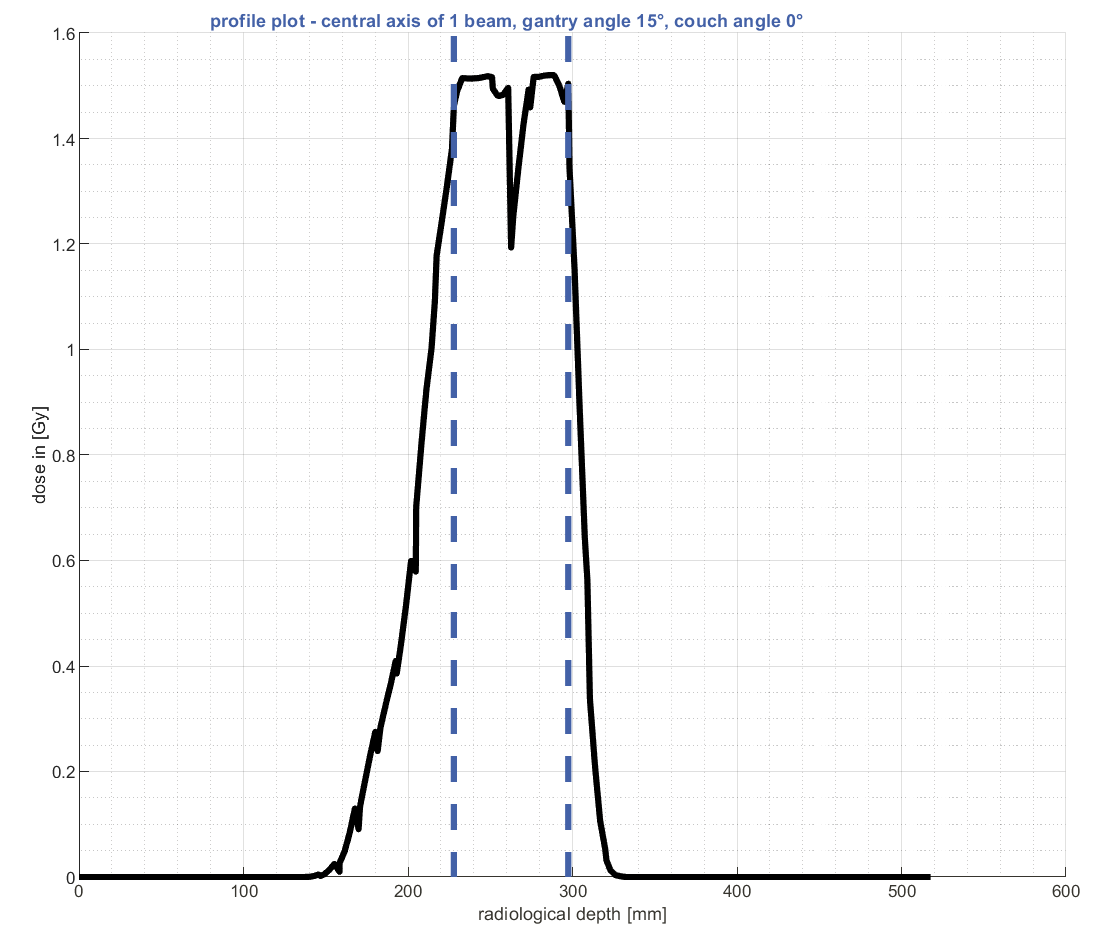
\includegraphics[width=\textwidth]{images/protons/protons_4_noeq_lateral.png}
                        \caption{Profilo lateral}
                        \label{fig:sub_protoni_4_no_profile_lateral}
                    \end{subfigure}\hfill
                    \caption{Profili del fascio di protoni}
                    \label{fig:protoni_4_no_profiles}
                \end{figure}
                \begin{figure}[H]
                    \centering
                    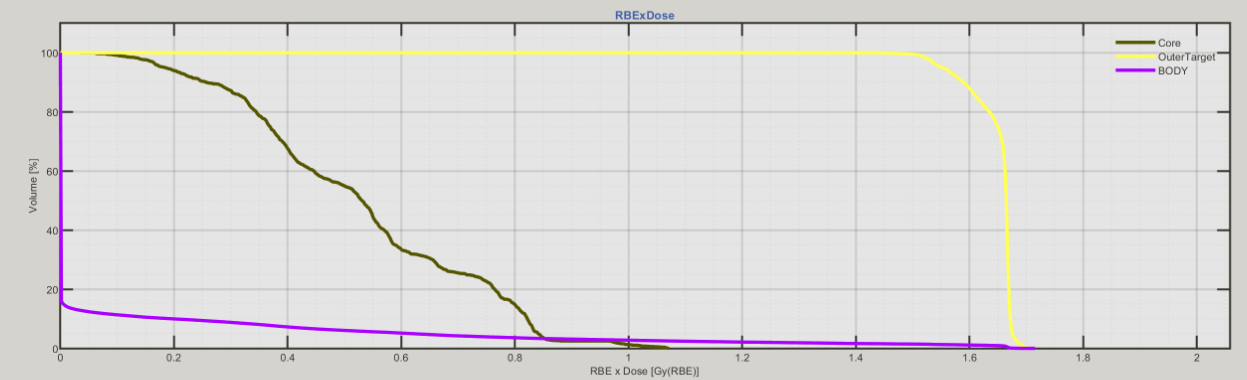
\includegraphics[width=0.6\textwidth]{images/protons/protons_4_noeq_DVH_graph.png}
                    \caption{Grafico DVH}
                    \label{fig:protoni_4_no_DVH_graph}
                \end{figure}
                \begin{table}[H]
                    \centering
                    \label{tab:dati_terza_misura_protoni}
                    \begin{tabular}{
                        l | c | c | c | c | c |
                    }
                    \toprule
                    & Mean & Std & Max & Min & D$_{98}$ \\
                    \midrule
                    Core & 0.5302 & 0.2132 & 1.0723 & 0.0355 & 0.1391 \\
                    Outer target & 1.6485 & 0.0390 & 1.7160 & 1.4210 & 1.5156 \\
                    Body & 0.0800 & 0.2732 & 1.7160 & 0 & 0 \\
                    \bottomrule
                    \end{tabular}
                    \caption{Dati ottenuti dalle curve di isodose (unità di misura della tabella [\unit{\gray}])}
                \end{table}

            \subsubsection{Ioni carbonio}
                \begin{figure}[H]
                    \centering
                    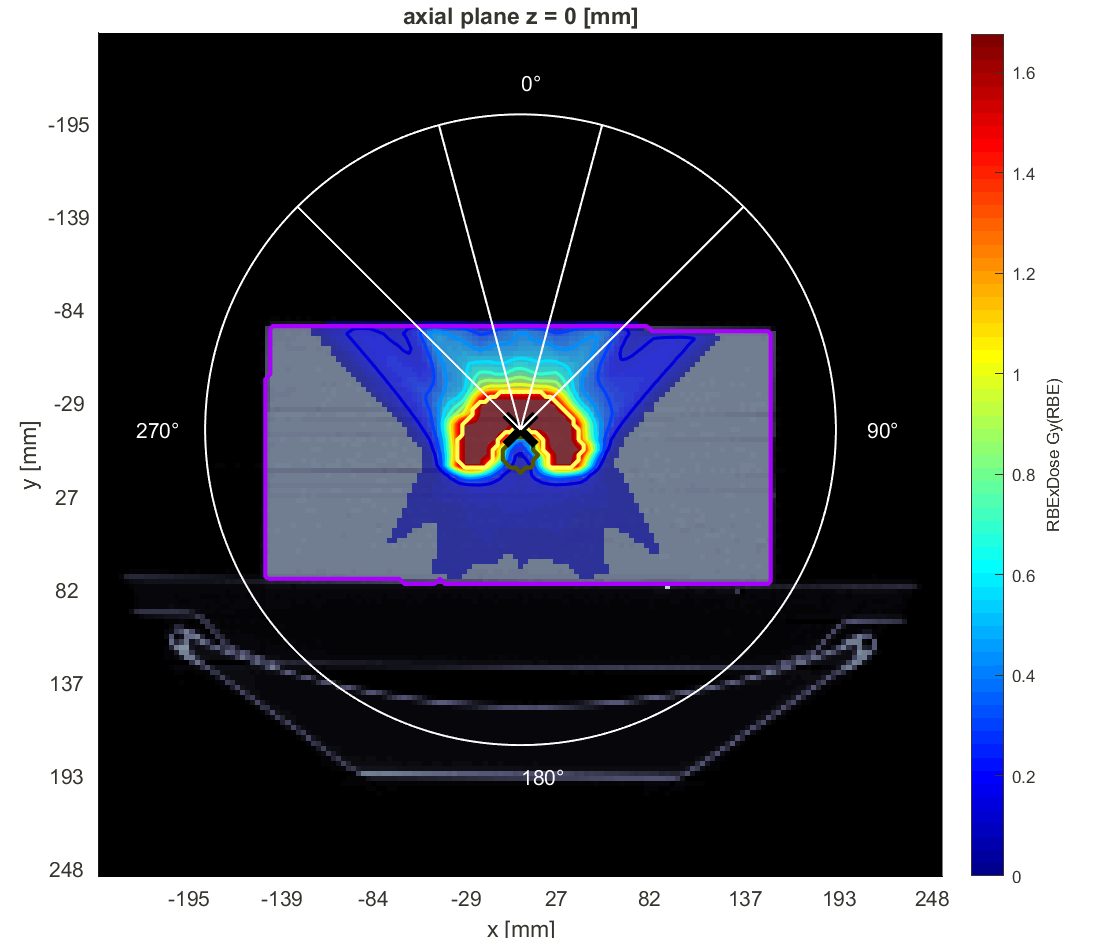
\includegraphics[width=0.6\textwidth]{images/carbon/carbon_4_noeq_intensity.png}
                    \caption{Ioni carbonio}
                    \label{fig:carbonio_4_no}
                \end{figure}
                \begin{figure}[H]
                    \centering
                    \begin{subfigure}{0.5\textwidth}
                        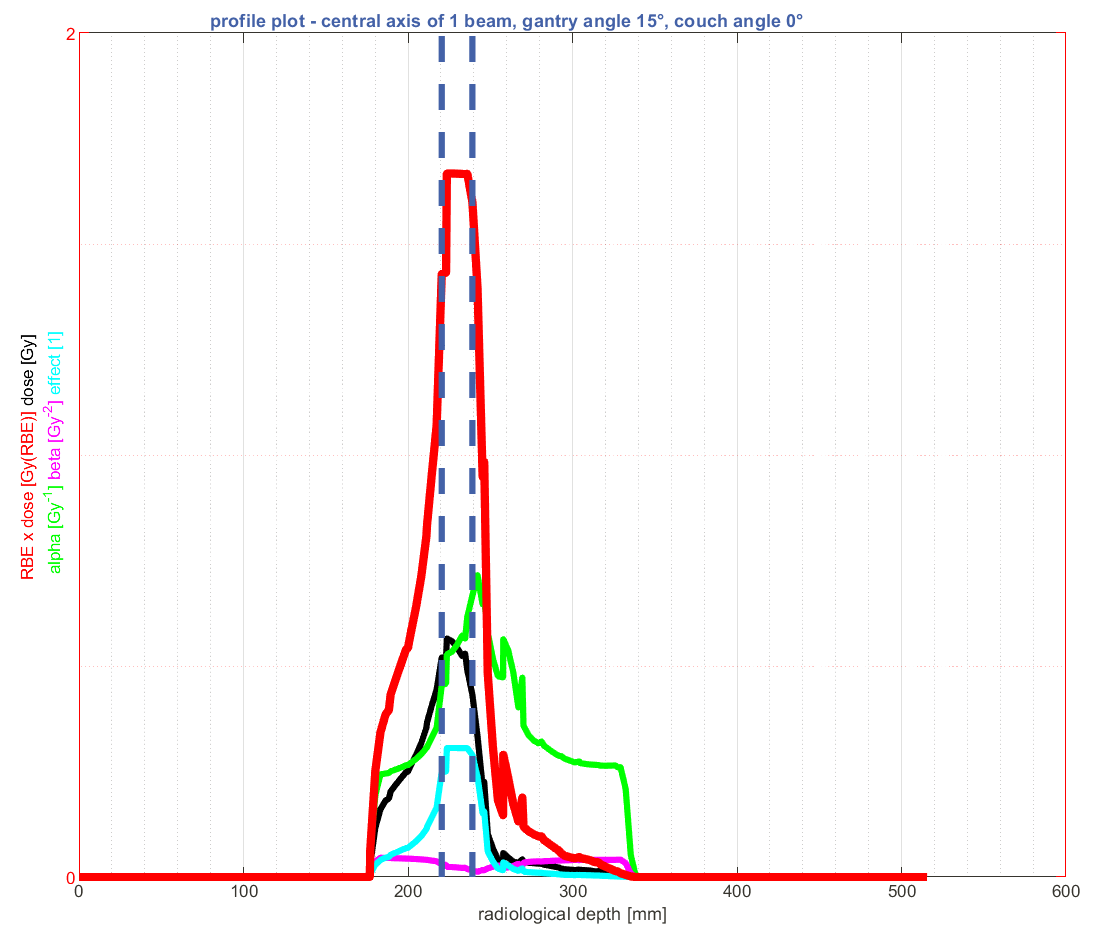
\includegraphics[width=\textwidth]{images/carbon/carbon_4_noeq_depth.png}
                        \caption{Profilo depth}
                        \label{fig:sub_carbonio_4_no_profile_depth}
                    \end{subfigure}\hfill
                    \begin{subfigure}{0.5\textwidth}
                        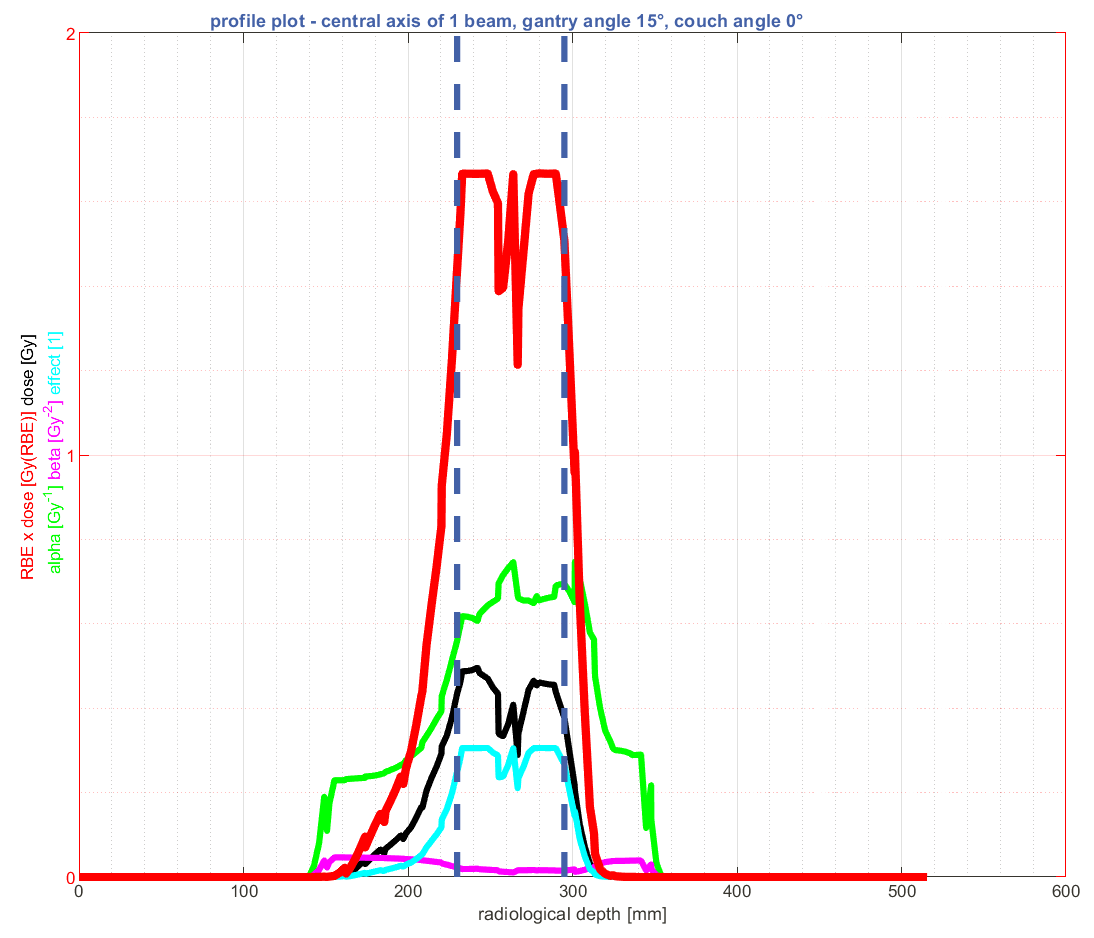
\includegraphics[width=\textwidth]{images/carbon/carbon_4_noeq_lateral.png}
                        \caption{Profilo lateral}
                        \label{fig:sub_carbonio_4_no_profile_lateral}
                    \end{subfigure}\hfill
                    \caption{Profili del fascio di ioni carbonio}
                    \label{fig:carbonio_4_no_profiles}
                \end{figure}
                \begin{figure}[H]
                    \centering
                    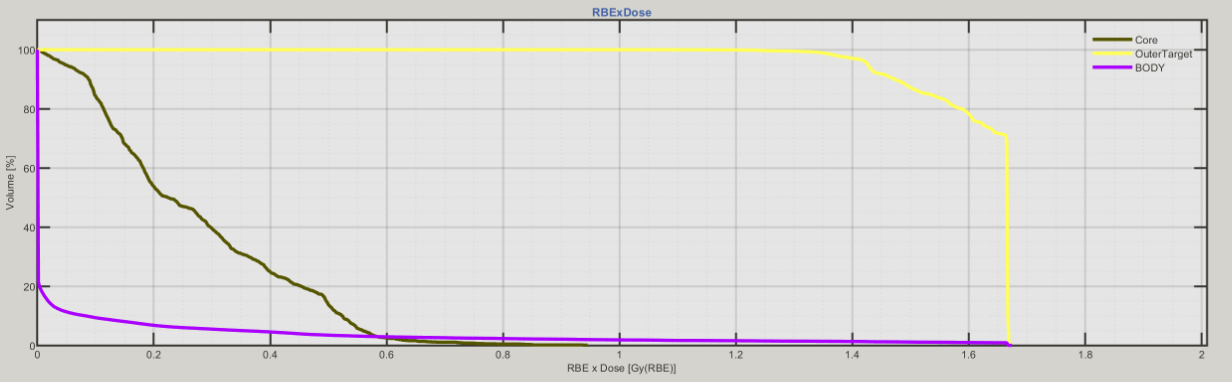
\includegraphics[width=0.6\textwidth]{images/carbon/carbon_4_noeq_DVH_graph.png}
                    \caption{Grafico DVH}
                    \label{fig:carbon_4_no_DVH_graph}
                \end{figure}
                \begin{table}[H]
                    \centering
                    \label{tab:dati_terza_misura_carbonio}
                    \begin{tabular}{
                        l | c | c | c | c | c |
                    }
                    \toprule
                    & Mean & Std & Max & Min & D$_{98}$ \\
                    \midrule
                    Core & 0.2716 & 0.1728 & 0.9459 & 0.0048 & 0.0204 \\
                    Outer target & 1.6231 & 0.0850 & 1.6749 & 1.1030 & 1.3718 \\
                    Body & 0.0571 & 0.2278 & 1.6749 & 0 & 0 \\
                    \bottomrule
                    \end{tabular}
                    \caption{Dati ottenuti dalle curve di isodose (unità di misura della tabella [\unit{\gray}])}
                \end{table}     
            
        \subsection{4 fasci equidistanziati di protoni con diversa bixel width}
            \begin{figure}[H]
                \centering
                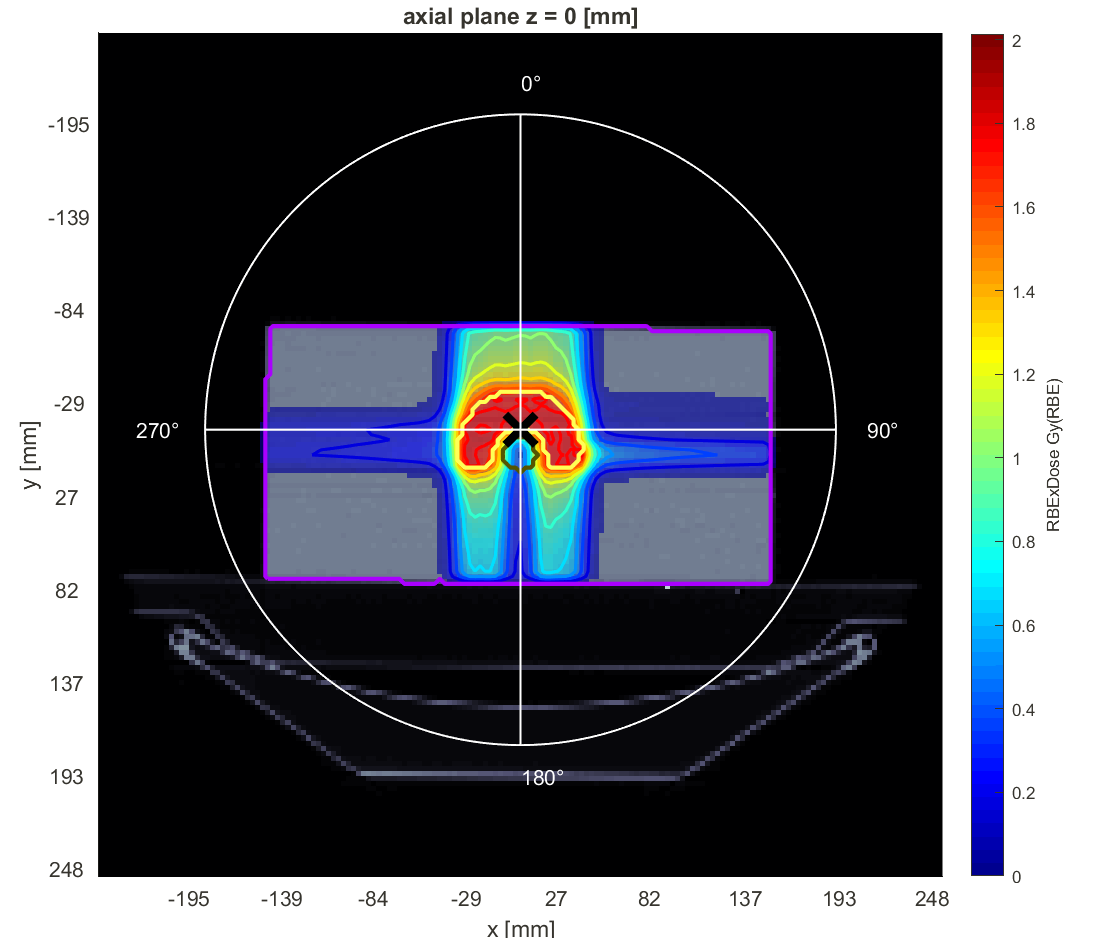
\includegraphics[width=0.6\textwidth]{images/protons/protons_4_eq_15bixel_intensity.png}
                \caption{Intensità fasci di protoni con bixel width 15 mm}
                \label{fig:protons_15bixel}
            \end{figure}
            \begin{figure}[H]
                \begin{subfigure}{0.5\textwidth}
                    \centering
                    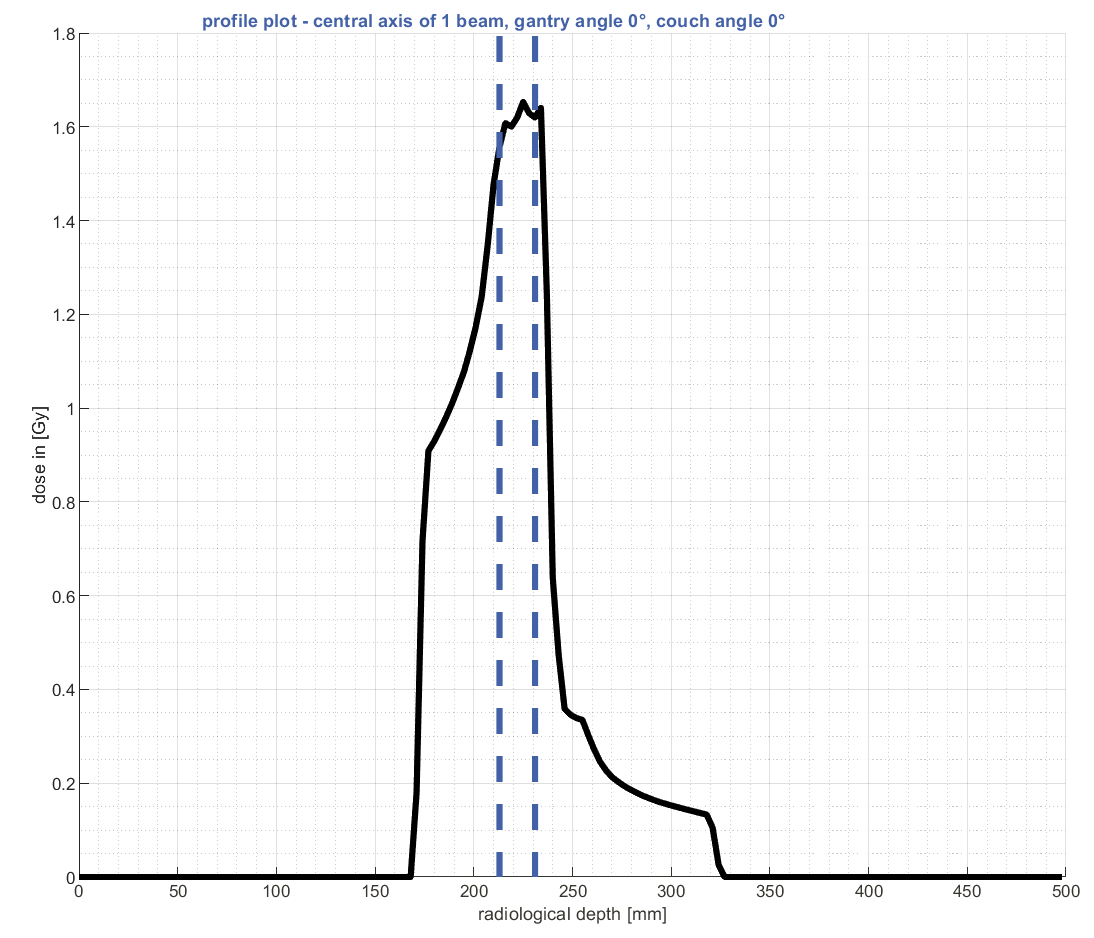
\includegraphics[width=\textwidth]{images/protons/protons_4_eq_15bixel_depth.png}
                    \caption{Profilo depth}
                    \label{fig:sub_protons_15_bixel_profile_depth}
                \end{subfigure}\hfill
                \begin{subfigure}{0.5\textwidth}
                    \centering
                    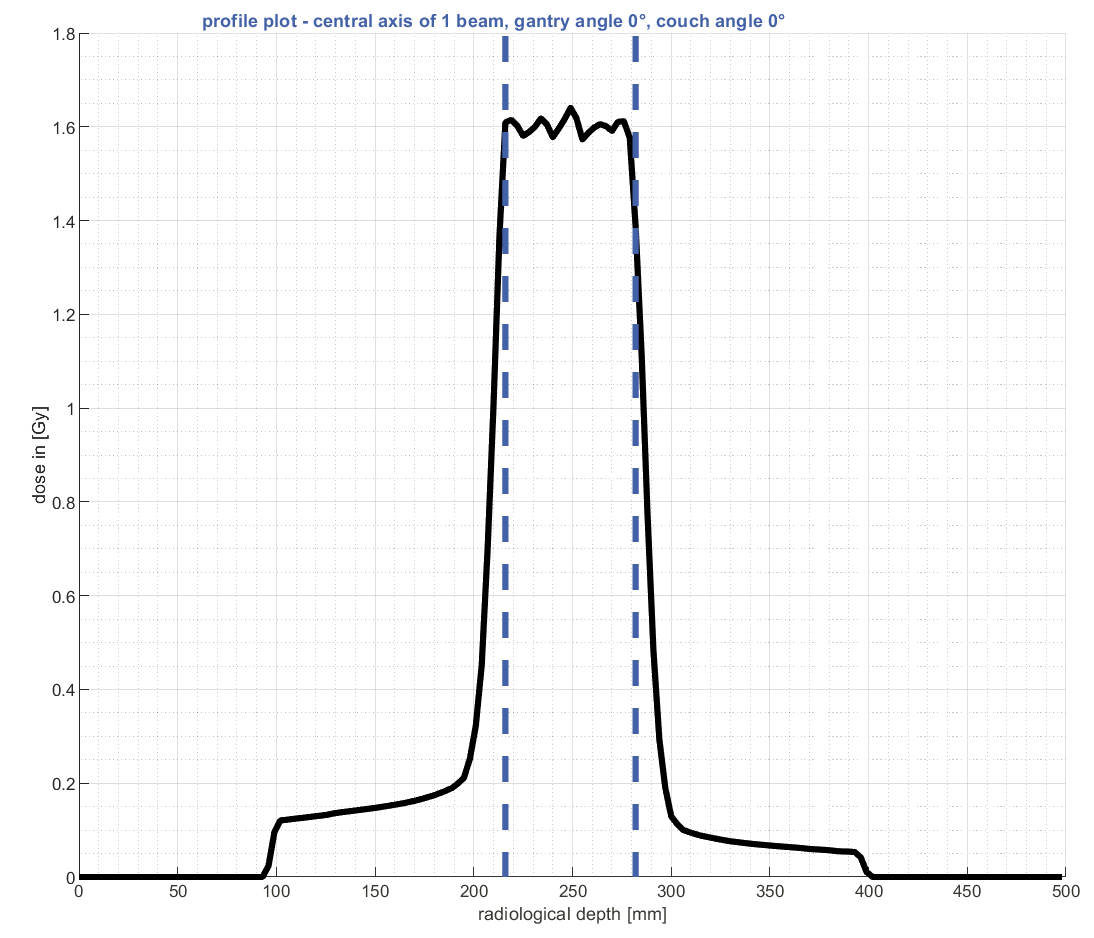
\includegraphics[width=\textwidth]{images/protons/protons_4_eq_15bixel_lateral.png}
                    \caption{Profilo lateral}
                    \label{fig:sub_protons_15_bixel_profile_lateral}
                \end{subfigure}\hfill
                \caption{Profili fasci protoni con bixel width di 15 mm}
                \label{fig:protons_15bixel_profiles}
            \end{figure}
            \begin{figure}
                \centering
                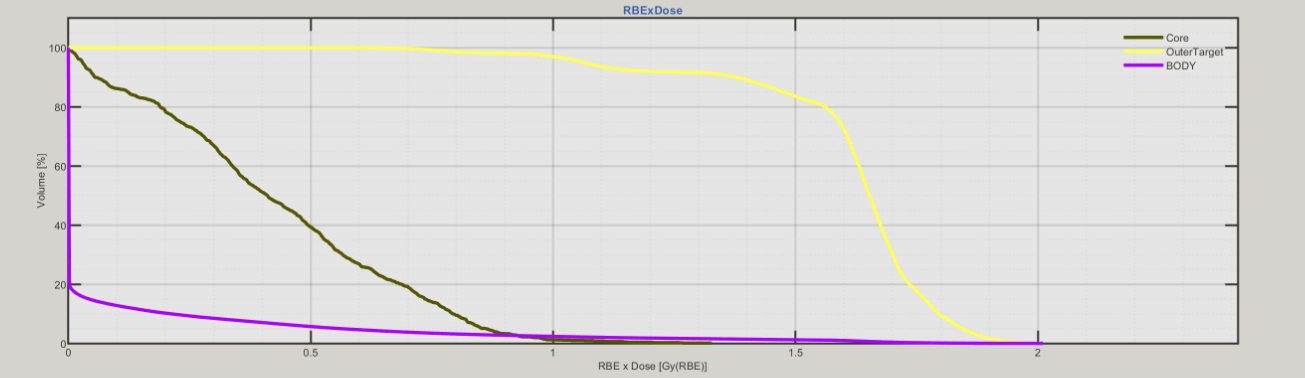
\includegraphics[width=0.6\textwidth]{images/protons/protons_4_eq_15bixel_DVH_graph.png}
                \caption{Grafico DVH}
                \label{fig:protons_15bixel_DVH_graph}
            \end{figure}
            \begin{table}[H]
                \centering
                \label{tab:dati_quarta_misura}
                \begin{tabular}{
                    l | c | c | c | c | c |
                }
                    \toprule
                    & Mean & Std & Max & Min & D$_{98}$ \\
                    \midrule
                    Core & 0.4311 & 0.2631 & 1.3284 & \num{5.6289e-04} & 0.0131 \\
                    Outer target & 1.6071 & 0.2162 & 2.0113 & 0.5984 & 0.9447 \\
                    Body & 0.0788 & 0.2609 & 2.0113 & 0 & 0 \\
                    \bottomrule
                \end{tabular}
                \caption{Dati ottenuti dalle curve di isodose (unità di misura della tabella [\unit{\gray}])}
            \end{table}

        \subsection{3 fasci di protoni non equidistanziati con scambio OAR-target}
            \begin{figure}[H]
                \centering
                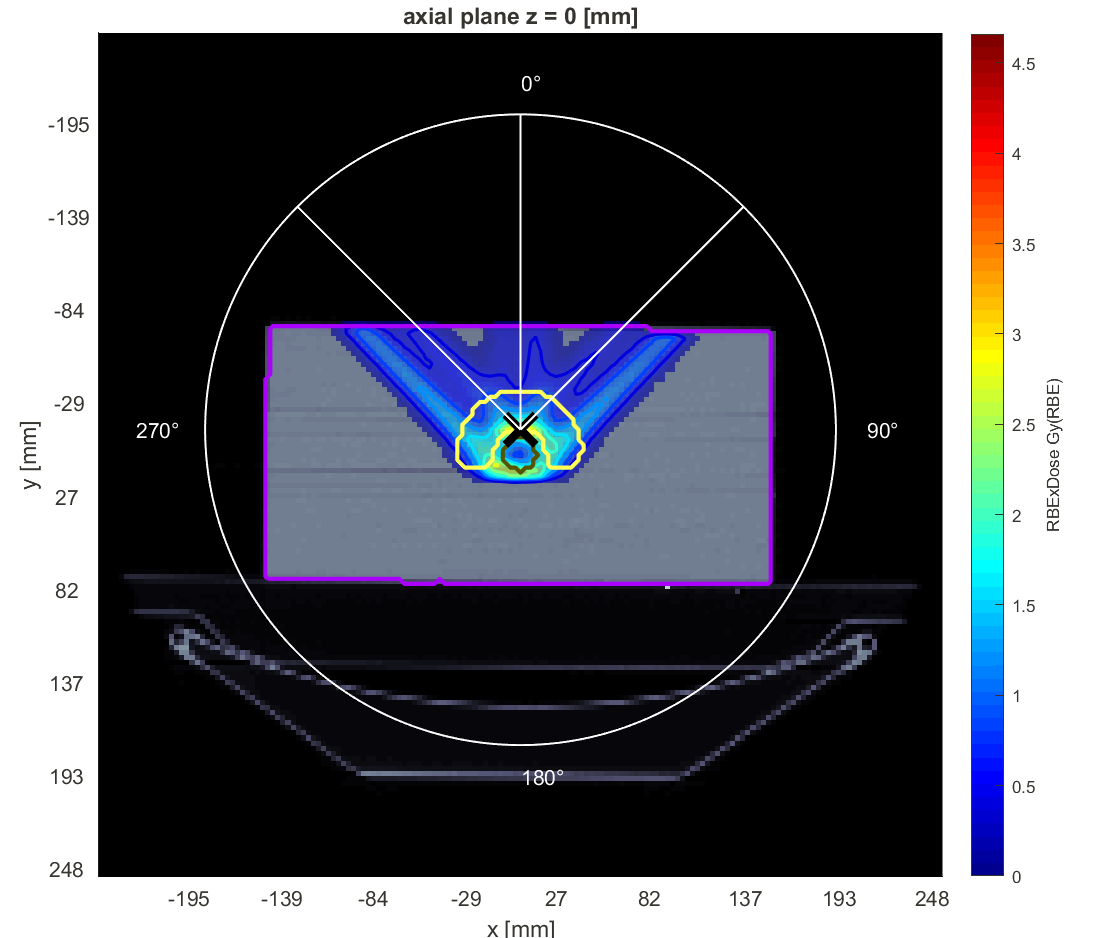
\includegraphics[width=0.6\textwidth]{images/protons/protons_3_noeq_inverted_intensity.png}
                \caption{Intensità fasci di protoni con scambio OAR-target}
                \label{fig:protons_inverted}
            \end{figure}
            \begin{figure}[H]
                \begin{subfigure}{0.5\textwidth}
                    \centering
                    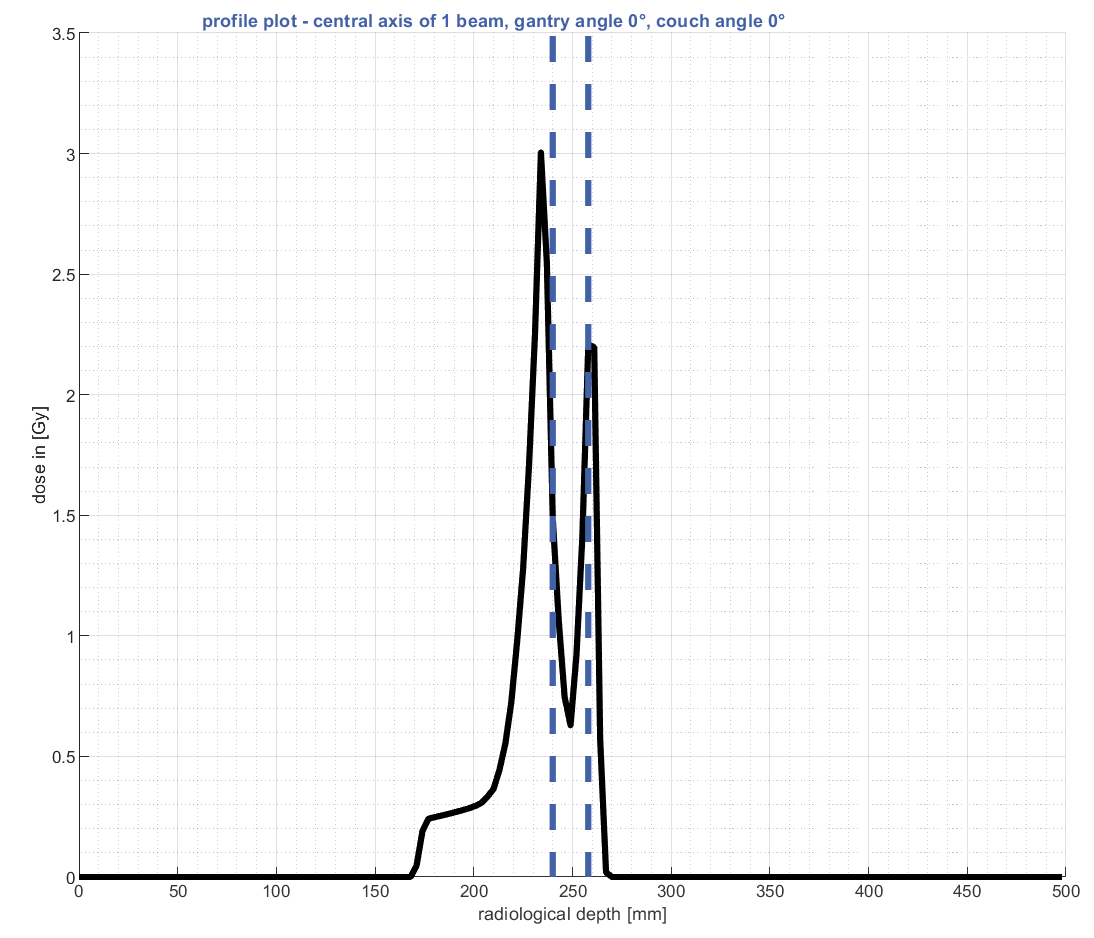
\includegraphics[width=\textwidth]{images/protons/protons_3_noeq_inverted_depth.png}
                    \caption{Profilo depth}
                    \label{fig:sub_protons_inverted_profile_depth}
                \end{subfigure}\hfill
                \begin{subfigure}{0.5\textwidth}
                    \centering
                    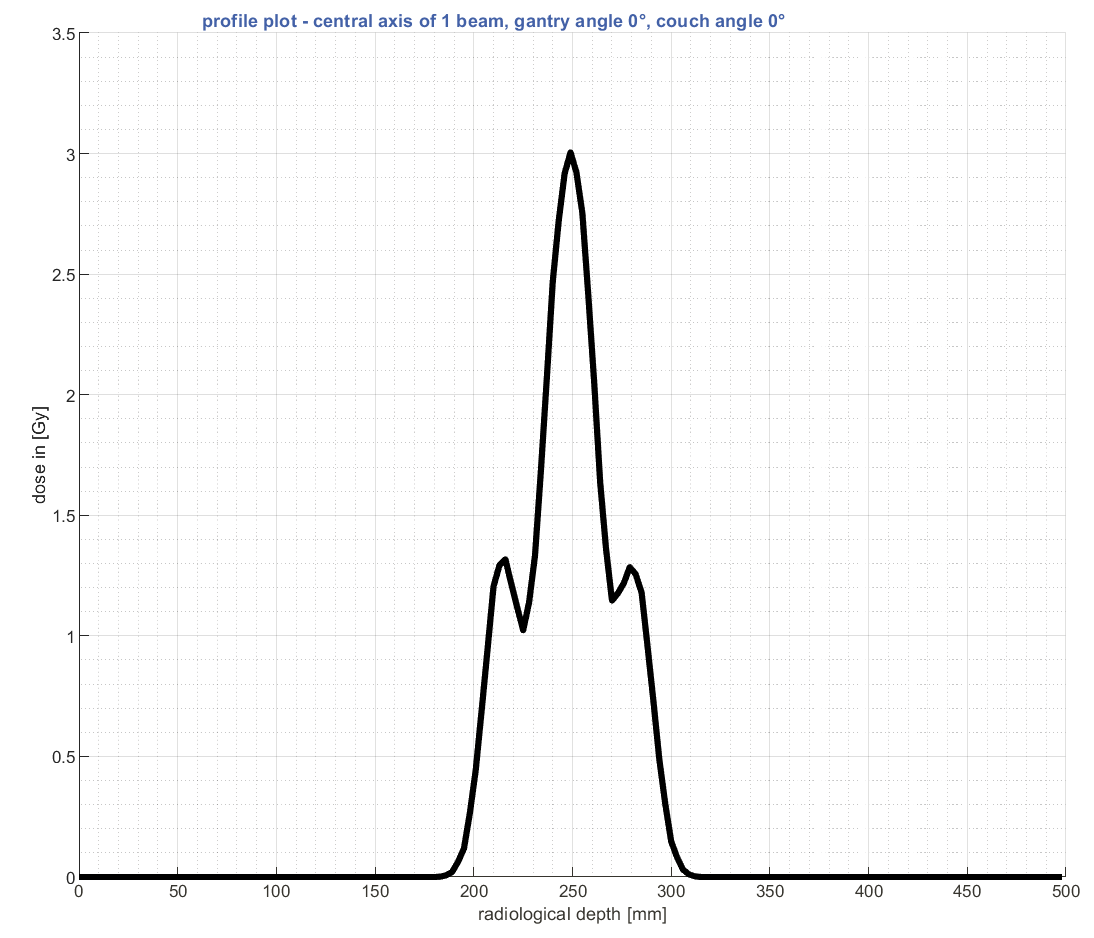
\includegraphics[width=\textwidth]{images/protons/protons_3_noeq_inverted_lateral.png}
                    \caption{Profilo lateral}
                    \label{fig:sub_protons_inverted_profile_lateral}
                \end{subfigure}\hfill
                \caption{Profili fasci protoni con scambio OAR-target}
                \label{fig:protons_inverted_profiles}
            \end{figure}
            \begin{figure}
                \centering
                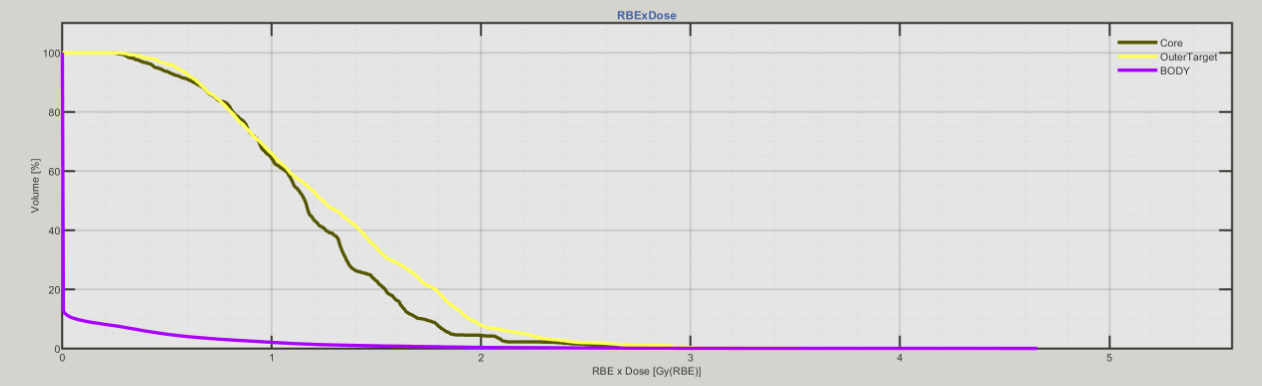
\includegraphics[width=0.6\textwidth]{images/protons/protons_3_noeq_inverted_DVH_graph.png}
                \caption{Grafico DVH}
                \label{fig:protons_inverted_DVH_graph}
            \end{figure}
            \begin{table}[H]
                \centering
                \label{tab:dati_quinta_misura}
                \begin{tabular}{
                    l | c | c | c | c | c |
                }
                    \toprule
                    & Mean & Std & Max & Min & D$_{98}$ \\
                    \midrule
                    Core & 1.1759 & 0.4442 & 2.7299 & 0.2497 & 0.3430 \\
                    Outer target & 1.2918 & 0.5279 & 3.6538 & 0.2237 & 0.4302 \\
                    Body & 0.0659 & 0.2635 & 4.6558 & 0 & 0 \\
                    \bottomrule
                \end{tabular}
                \caption{Dati ottenuti dalle curve di isodose (unità di misura della tabella [\unit{\gray}])}
            \end{table}

        \subsection{Caso clinico}
            \subsubsection{Fotoni}
                \begin{figure}[H]
                    \centering
                    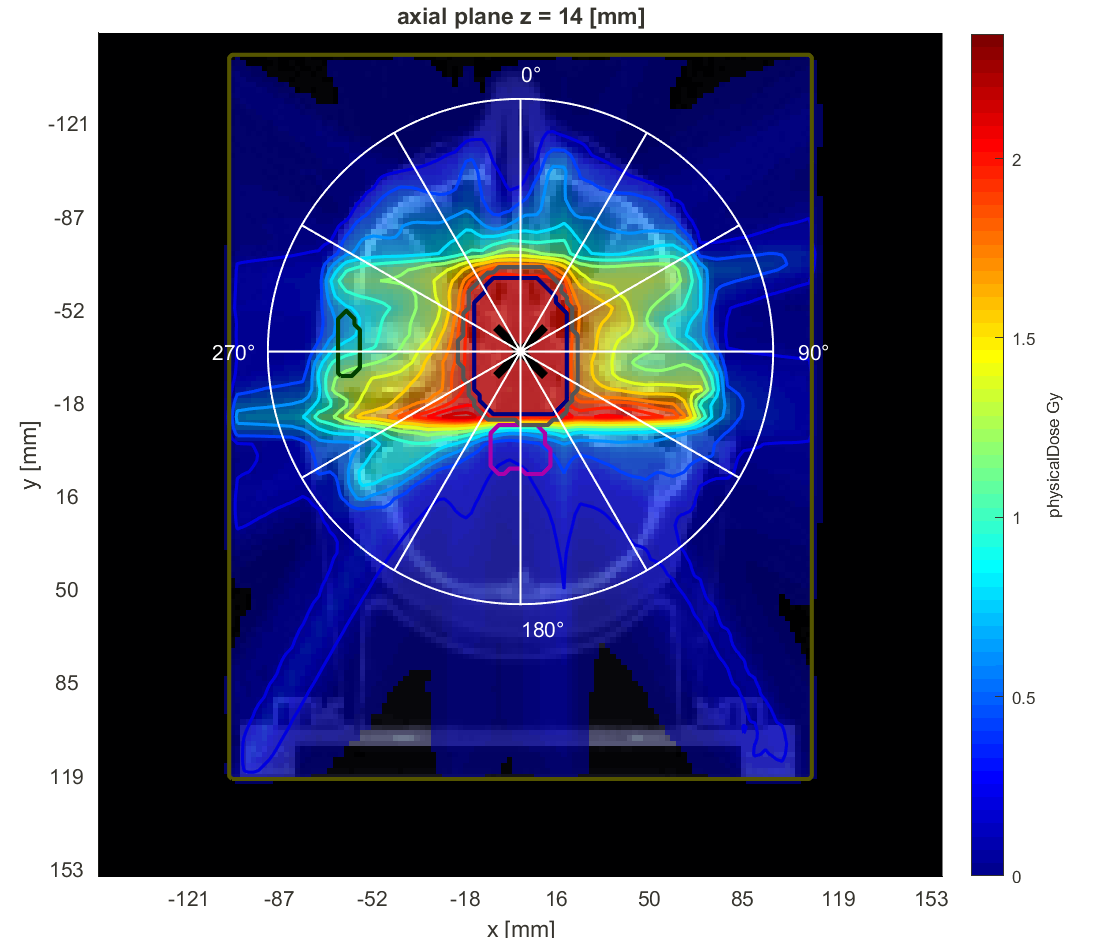
\includegraphics[width=0.6\textwidth]{images/photons/photons_best_intensity.png}
                    \caption{Intensità fasci fotoni}
                    \label{fig:sub_fotoni_best}
                \end{figure}
                \begin{figure}[H]
                    \centering
                    \begin{subfigure}{0.5\textwidth}
                        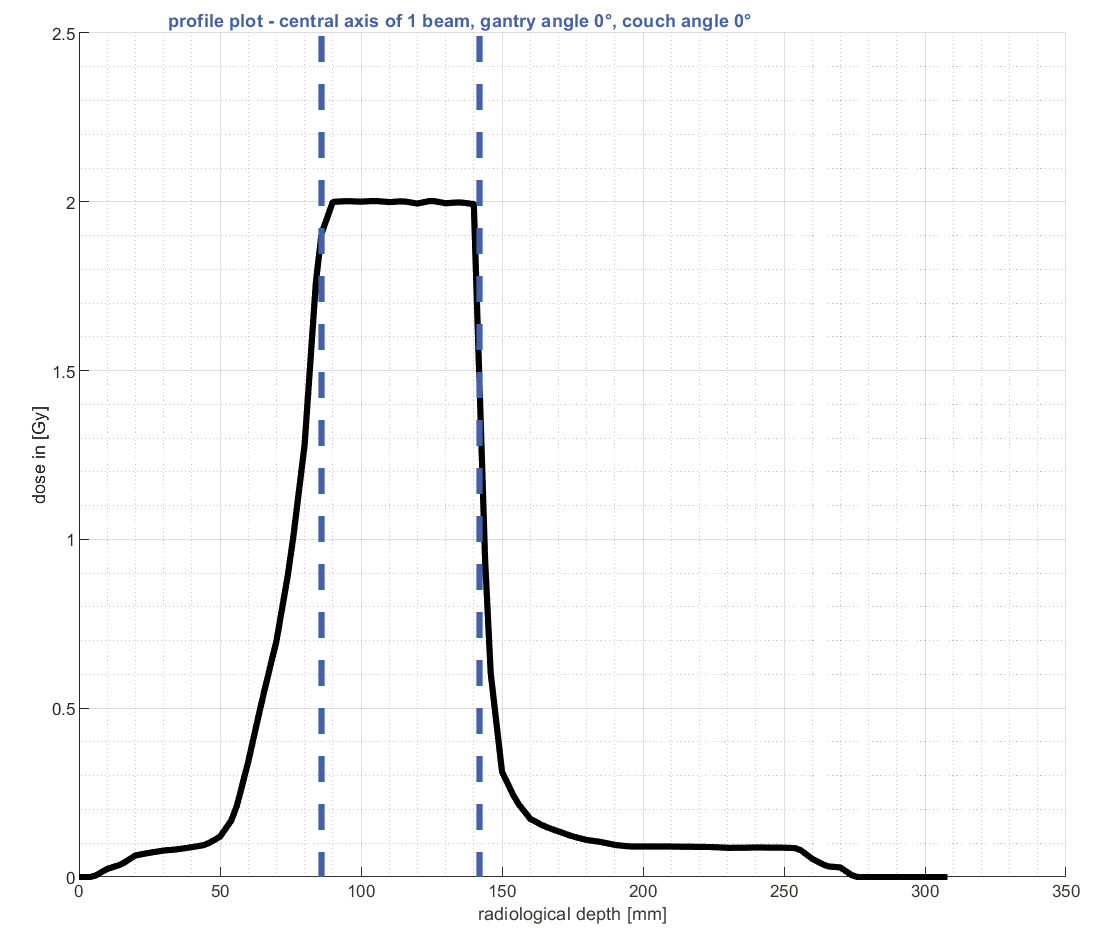
\includegraphics[width=\textwidth]{images/photons/photons_best_depth.png}
                        \caption{Profilo depth}
                        \label{fig:sub_fotoni_best_profile_depth}
                    \end{subfigure}\hfill
                    \begin{subfigure}{0.5\textwidth}
                        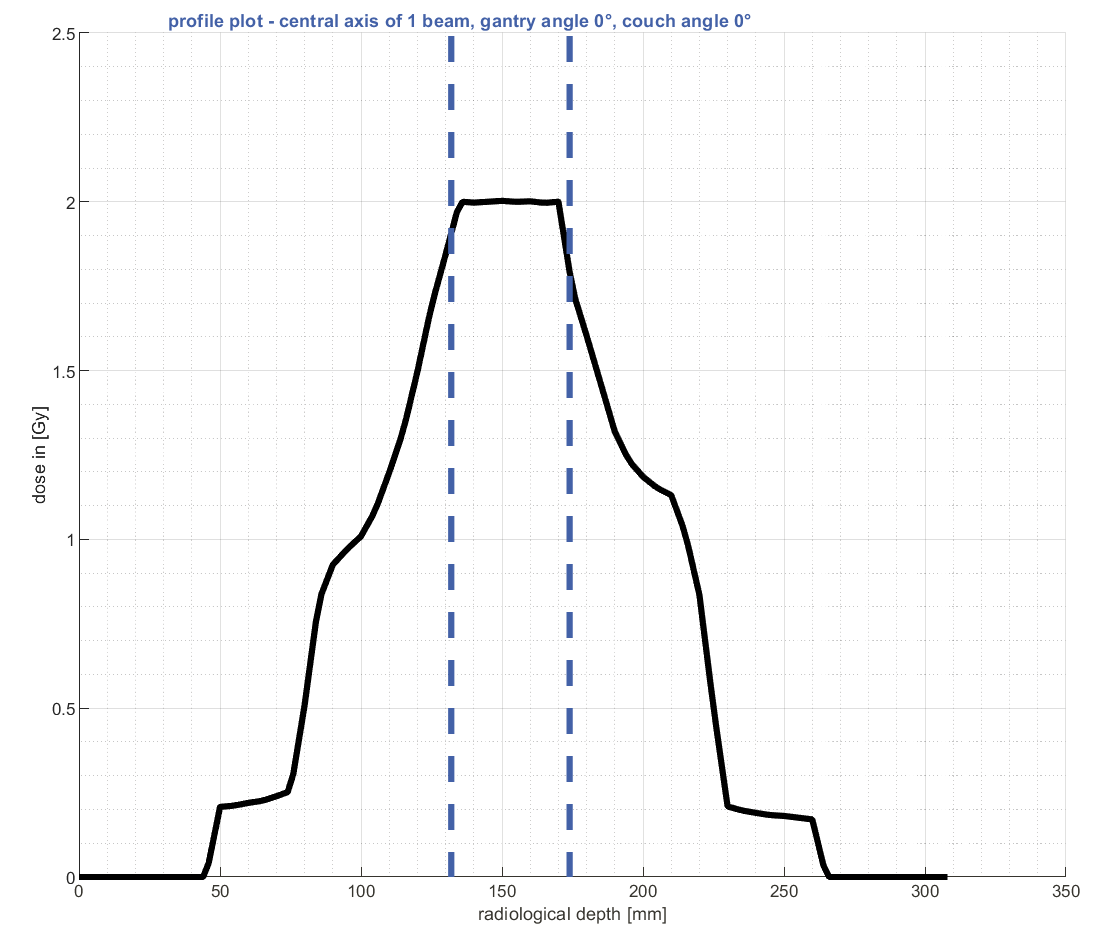
\includegraphics[width=\textwidth]{images/photons/photons_best_lateral.png}
                        \caption{Profilo lateral}
                        \label{fig:sub_fotoni_best_profile_lateral}
                    \end{subfigure}\hfill
                    \caption{Profili del fascio di fotoni}
                    \label{fig:fotoni_4_best_profiles}
                \end{figure}
                \begin{figure}[H]
                    \centering
                    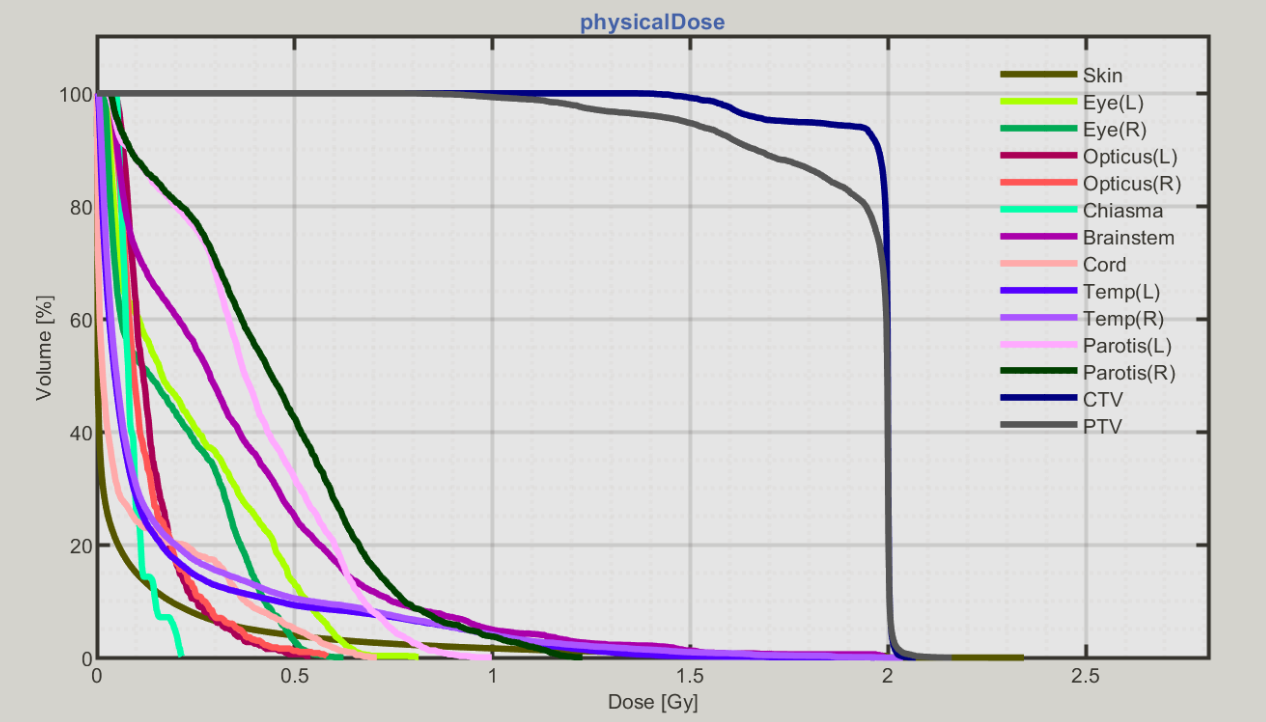
\includegraphics[width=0.6\textwidth]{images/photons/photons_best_DVH_graph.png}
                    \caption{Grafico DVH}
                    \label{fig:fotoni_best_DVH_graph}
                \end{figure}
                \begin{table}[H]
                        \centering
                        \label{tab:dati_caso_clinico_fotoni}
                        \begin{tabular}{
                            l | c | c | c | c | c |
                        }
                            \toprule
                            & Mean & Std & Max & Min & D$_{98}$\\
                            \midrule
                            Skin & 0.0739 & 0.2301 & 2.3447 & 0 & 0 \\
                            Left eye & 0.2324 & 0.1966 & 0.8141 & 0.0193 & 0.0285 \\
                            Right eye & 0.1910 & 0.1630 & 0.6253 & 0.0178 & 0.0219 \\
                            Left opticus & 0.1421 & 0.0867 & 0.5417 & 0.0479 & 0.0539 \\
                            Right opticus & 0.1314 & 0.1006 & 0.5820 & 0.0338 & 0.0388 \\
                            Chiasma & 0.0916 & 0.0392 & 0.2148 & 0.0494 & 0.0513 \\
                            Brainstem & 0.3581 & 0.3319 & 1.9929 & 0.0285 & 0.0389 \\
                            Cord & 0.1003 & 0.1676 & 0.7083 & 0 & 0 \\
                            Left Temp & 0.1538 & 0.2838 & 1.9688 & 0.0023 & 0.0046 \\
                            Right Temp & 0.1729 & 0.3100 & 2.0392 & 0.0037 & 0.0065 \\
                            Left Parotis & 0.3938 & 0.2116 & 1.0003 & 0.0282 & 0.0376 \\
                            Right Parotis & 0.4526 & 0.2624 & 1.2288 & 0.0329 & 0.0412 \\
                            CVT & 1.9759 & 0.0925 & 2.0718 & 1.3682 & 1.5813 \\
                            PVT & 1.9212 & 0.1942 & 2.1613 & 0.7805 & 1.1955 \\
                            \bottomrule
                        \end{tabular}
                        \caption{Dati ottenuti dalle curve di isodose (unità di misura della tabella [\unit{\gray}])}
                    \end{table}

            \subsubsection{Protoni}
                \begin{figure}[H]
                    \centering
                    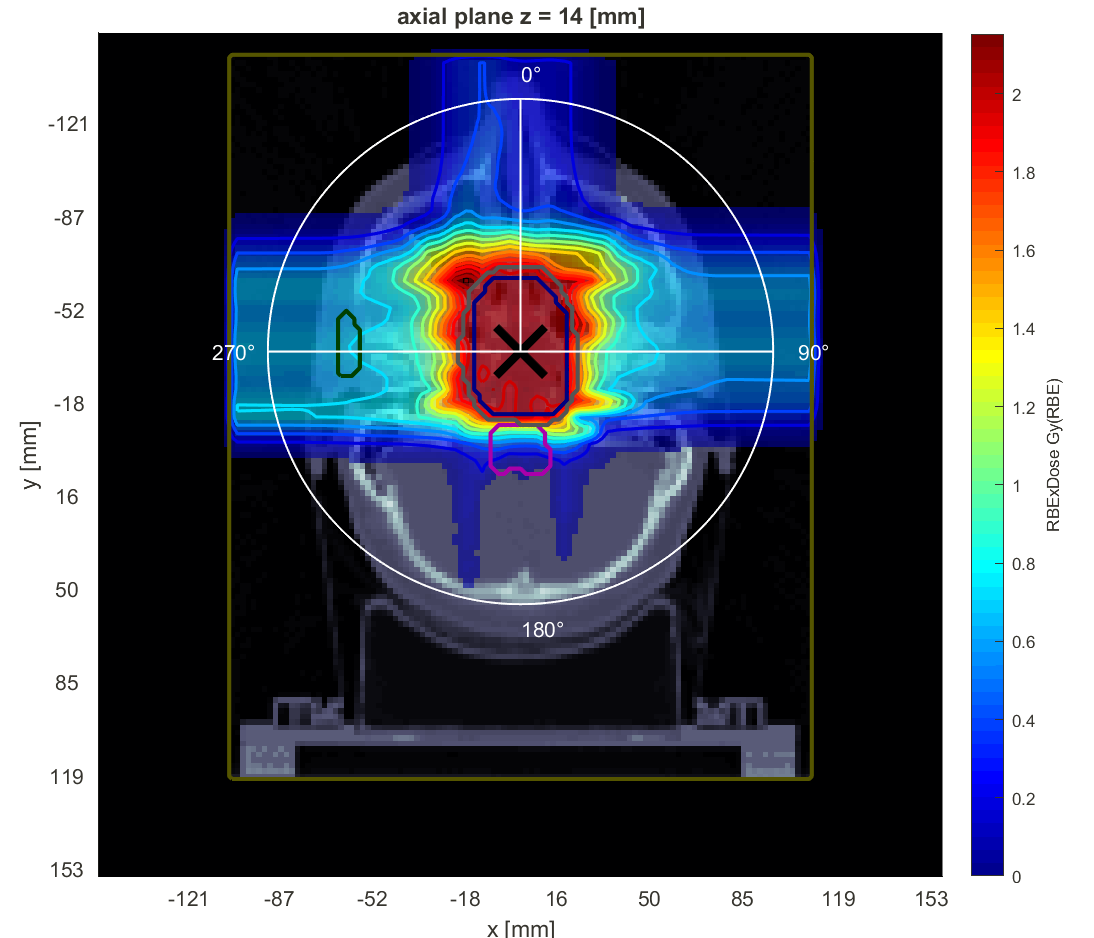
\includegraphics[width=0.6\textwidth]{images/protons/protons_best_intensity.png}
                    \caption{Intensità fasci protoni}
                    \label{fig:sub_protoni_best}
                \end{figure}
                \begin{figure}[H]
                    \centering
                    \begin{subfigure}{0.5\textwidth}
                        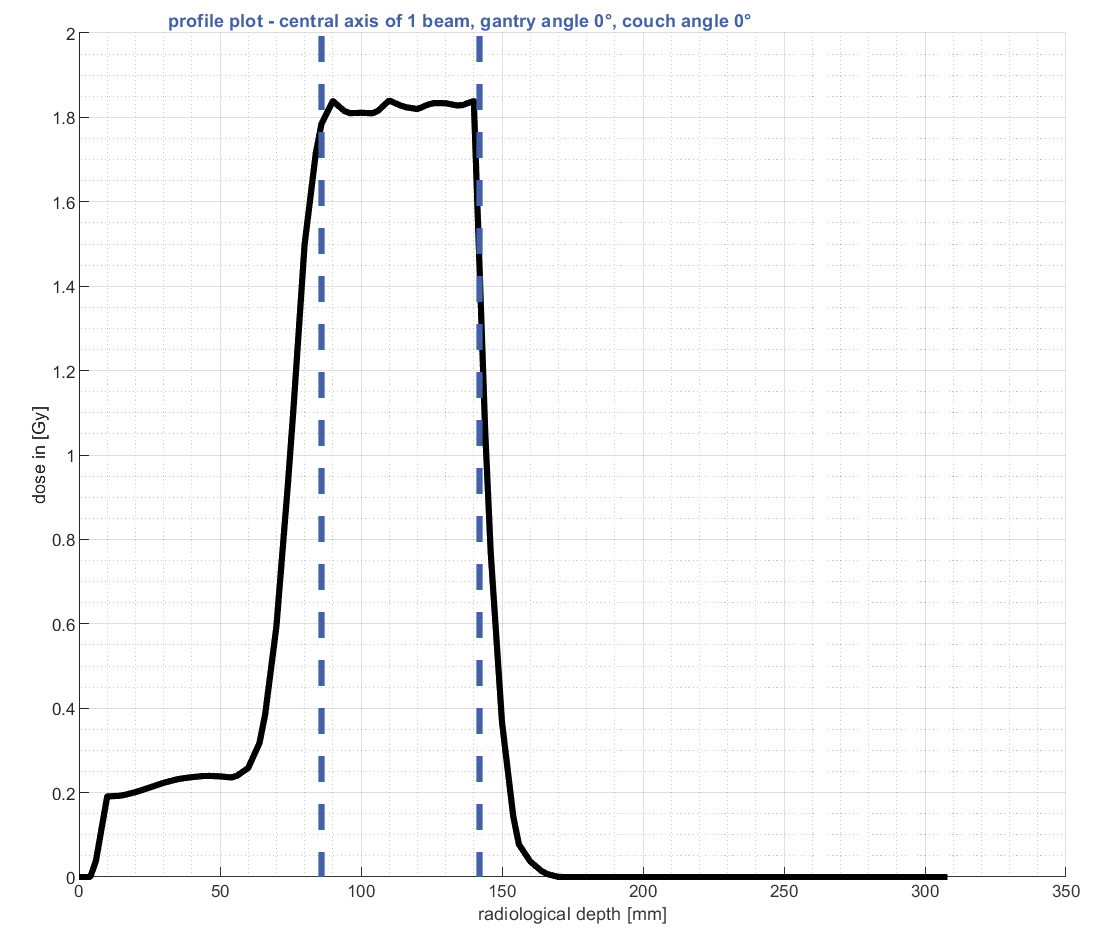
\includegraphics[width=\textwidth]{images/protons/protons_best_depth.png}
                        \caption{Profilo depth}
                        \label{fig:sub_protoni_best_profile_depth}
                    \end{subfigure}\hfill
                    \begin{subfigure}{0.5\textwidth}
                        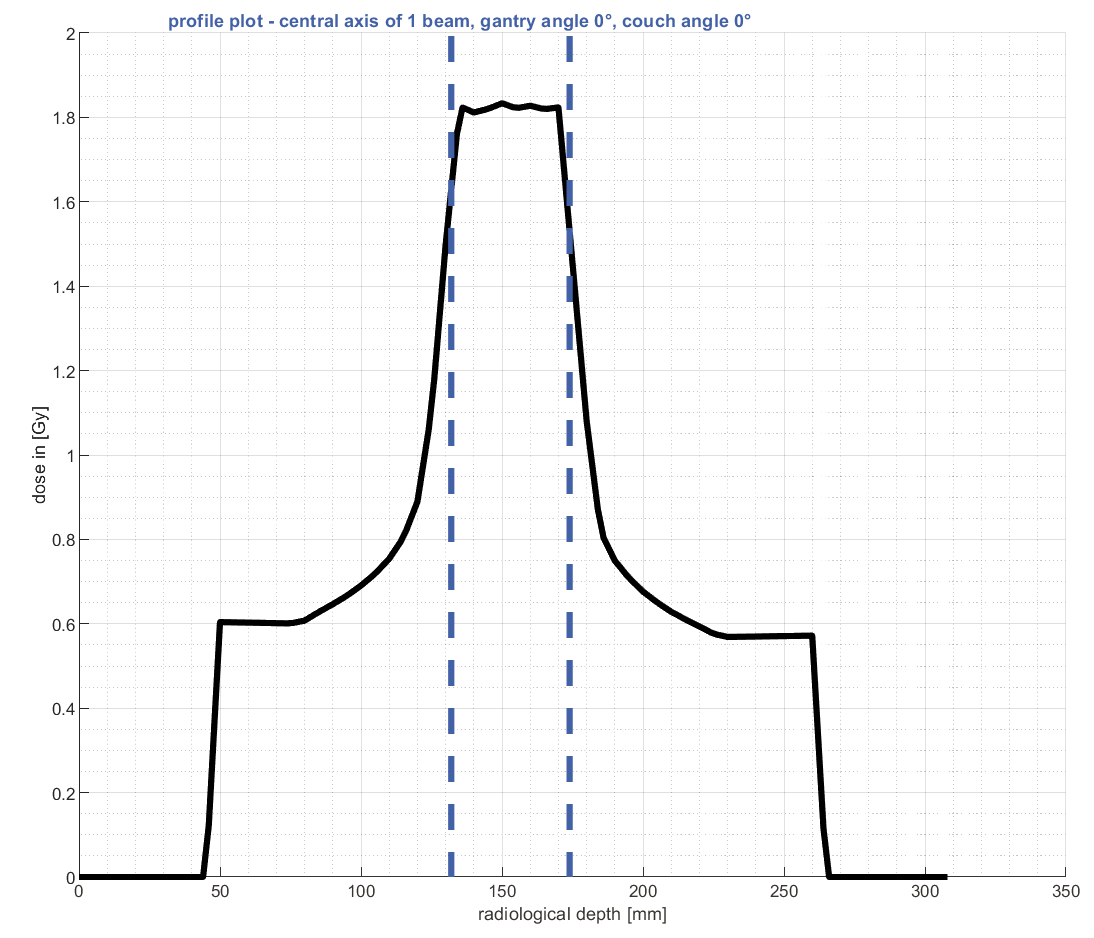
\includegraphics[width=\textwidth]{images/protons/protons_best_lateral.png}
                        \caption{Profilo lateral}
                        \label{fig:sub_protoni_best_profile_lateral}
                    \end{subfigure}\hfill
                    \caption{Profili dei fasci di protoni}
                    \label{fig:protoni_best_profiles}
                \end{figure}
                \begin{figure}[H]
                    \centering
                    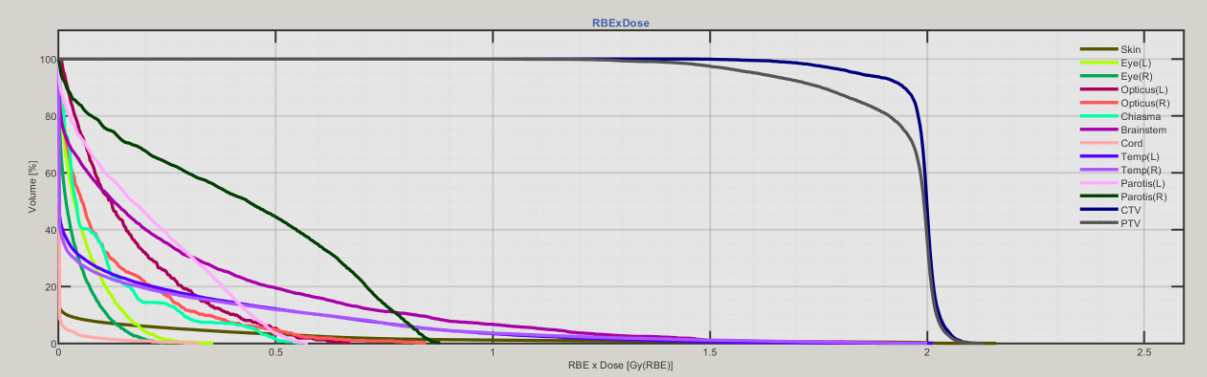
\includegraphics[width=0.6\textwidth]{images/protons/protons_best_DVH_graph.png}
                    \caption{Grafico DVH}
                    \label{fig:protoni_best_DVH_graph}
                \end{figure}
                \begin{table}[H]
                        \centering
                        \label{tab:dati_caso_clinico_protoni}
                        \begin{tabular}{
                            l | c | c | c | c | c |
                        }
                            \toprule
                            & Mean & Std & Max & Min & D$_{98}$\\
                            \midrule
                            Skin & 0.0451 & 0.2057 & 2.1599 & 0 & 0 \\
                            Left eye & 0.0594 & 0.0653 & 0.3575 & \num{2.3780e-07} & \num{1.3578e-04} \\
                            Right eye & 0.0384 & 0.0493 & 0.2499 & \num{2.9636e-09} & \num{2.5563e-08} \\
                            Left opticus & 0.1669 & 0.1516 & 0.6732 & 0.0060 & 0.081 \\
                            Right opticus & 0.1183 & 0.1569 & 0.8471 & \num{4.4614e-05} & \num{6.4607e-04} \\
                            Chiasma & 0.0994 & 0.1285 & 0.5607 & 0.0018 & 0.0029 \\
                            Brainstem & 0.2754 & 0.3659 & 1.9450 & 0 & \num{7.6896e-08} \\
                            Cord & 0.0052 & 0.0281 & 0.3236 & 0 & 0 \\
                            Left Temp & 0.1484 & 0.3057 & 2.0157 & 0 & 0 \\
                            Right Temp & 0.1462 & 0.3224 & 2.0012 & 0 & 0 \\
                            Left Parotis & 0.2002 & 0.1659 & 0.5764 & \num{5.1772e-07} & \num{1.4375e-04} \\
                            Right Parotis & 0.4092 & 0.2854 & 0.8803 & \num{9.6017e-05} & 0.0026 \\
                            CVT & 1.9849 & 0.0683 & 2.1310 & 1.4505 & 1.7322 \\
                            PVT & 1.9388 & 0.1401 & 2.1310 & 1.0040 & 1.4717 \\
                            \bottomrule
                        \end{tabular}
                        \caption{Dati ottenuti dalle curve di isodose (unità di misura della tabella [\unit{\gray}])}
                    \end{table}

            \subsubsection{Ioni carbonio}
                \begin{figure}[H]
                    \centering
                    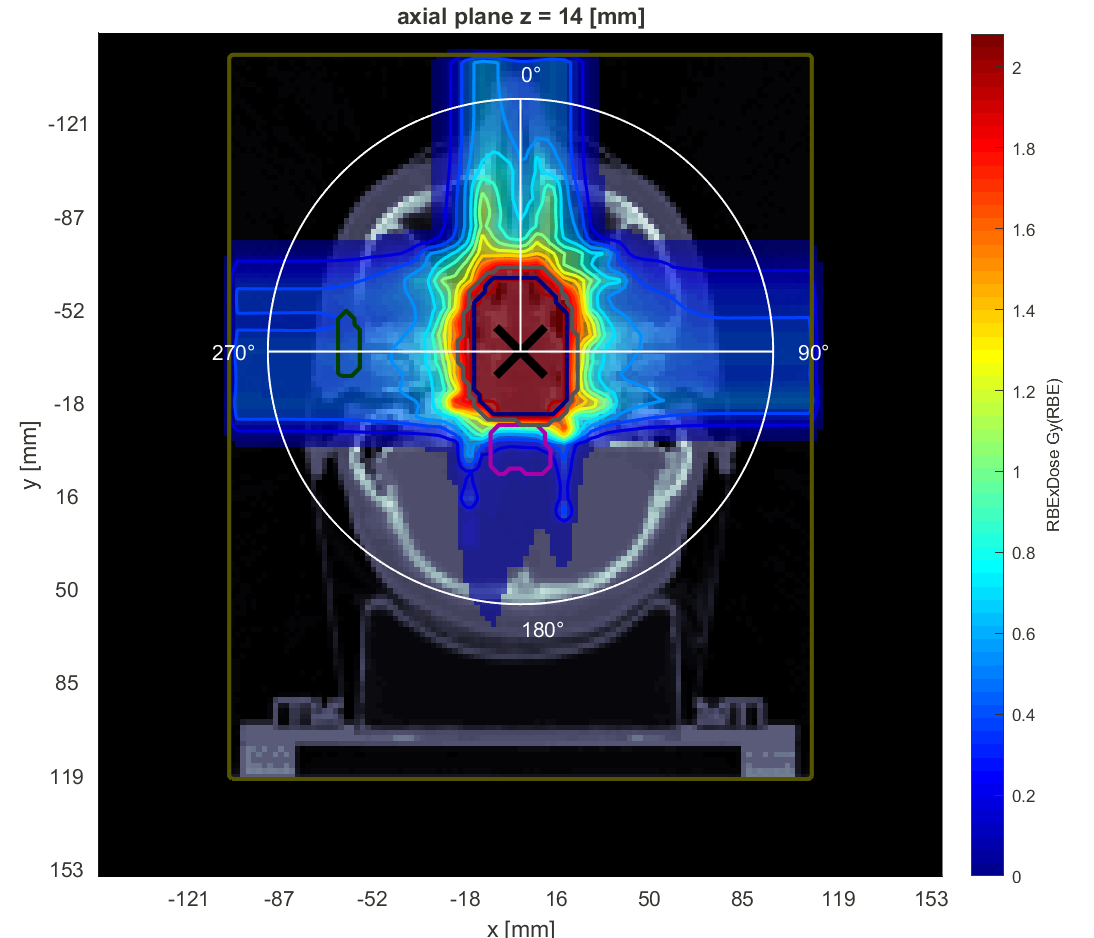
\includegraphics[width=0.6\textwidth]{images/carbon/carbon_best_intensity.png}
                    \caption{Intensità fasci ioni carbonio}
                    \label{fig:carbonio_best}
                \end{figure}
                \begin{figure}[H]
                    \centering
                    \begin{subfigure}{0.5\textwidth}
                        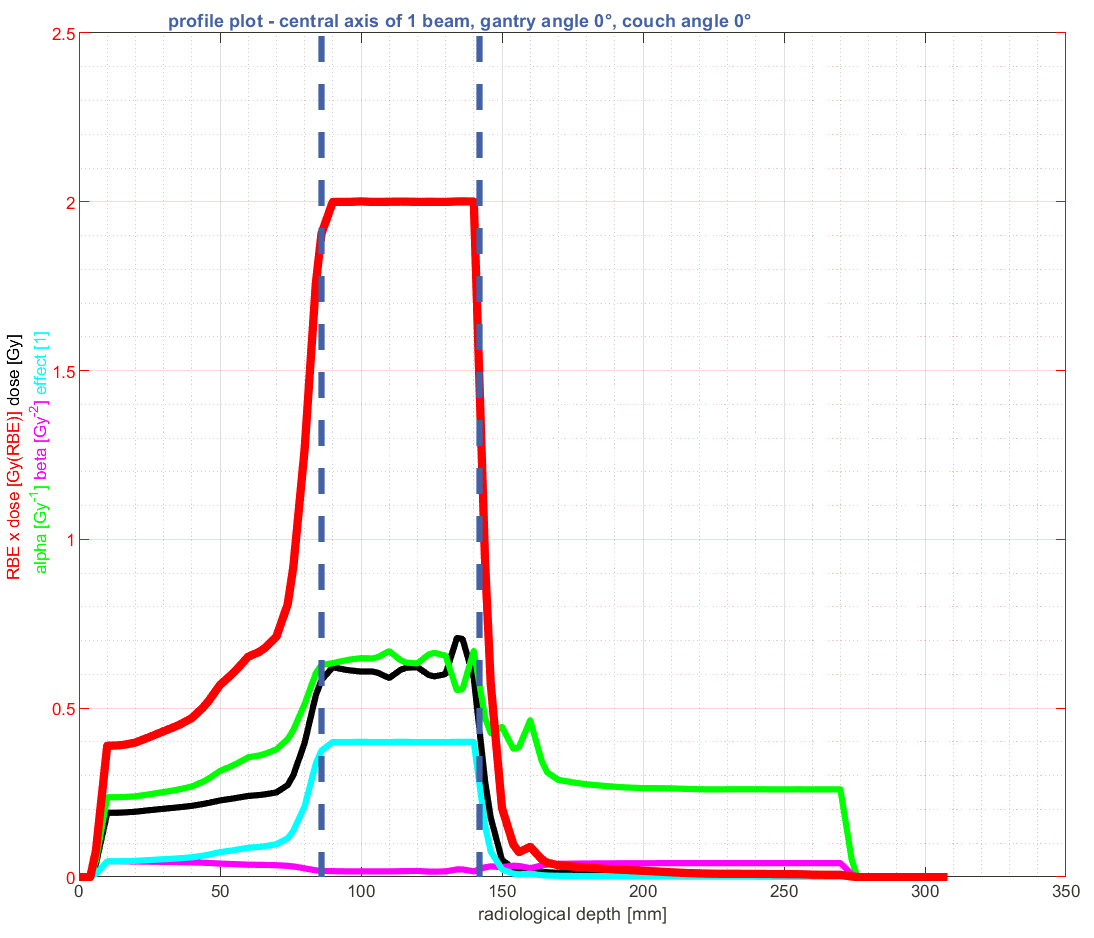
\includegraphics[width=\textwidth]{images/carbon/carbon_best_depth.png}
                        \caption{Profilo depth}
                        \label{fig:sub_carbonio_best_profile_depth}
                    \end{subfigure}\hfill
                    \begin{subfigure}{0.5\textwidth}
                        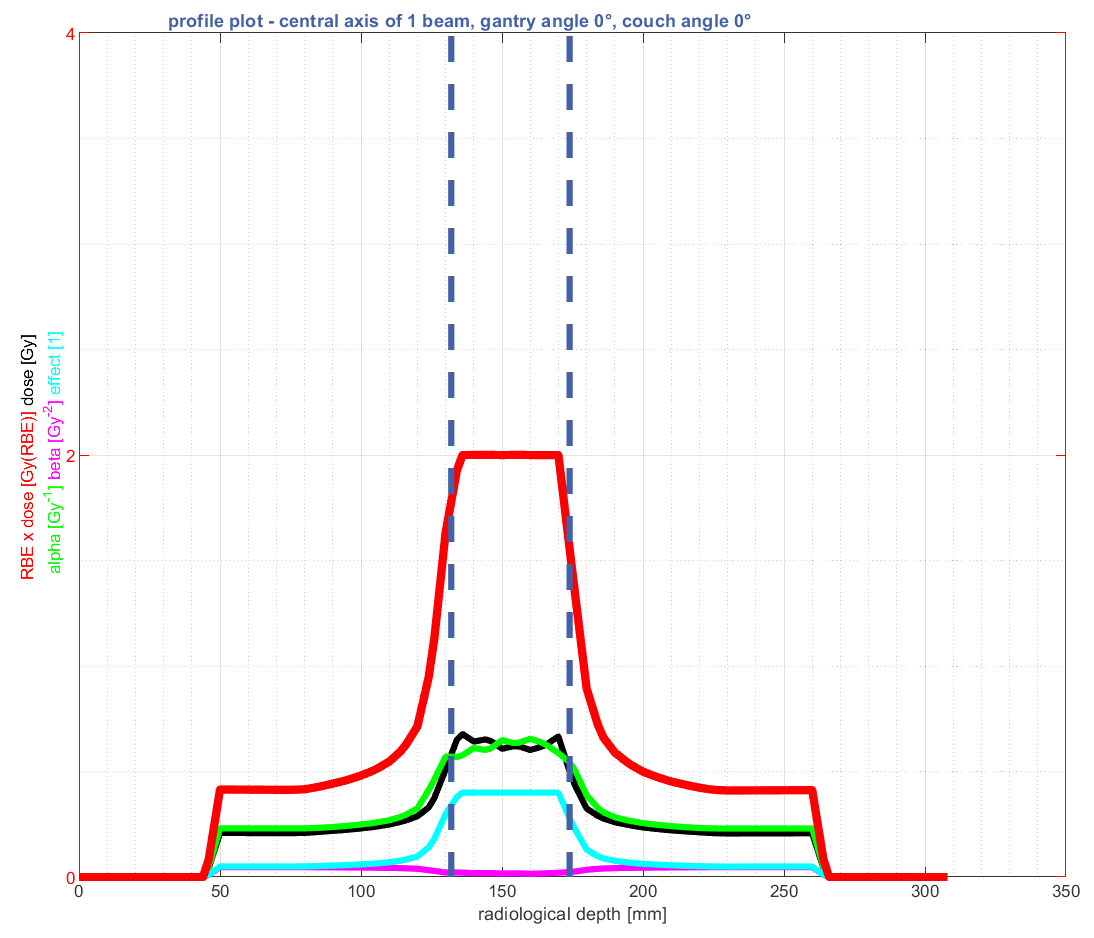
\includegraphics[width=\textwidth]{images/carbon/carbon_best_lateral.png}
                        \caption{Profilo lateral}
                        \label{fig:sub_carbonio_best_profile_lateral}
                    \end{subfigure}\hfill
                    \caption{Profili del fascio di ioni carbonio}
                    \label{fig:carbonio_best_profiles}
                \end{figure}
                \begin{figure}[H]
                    \centering
                    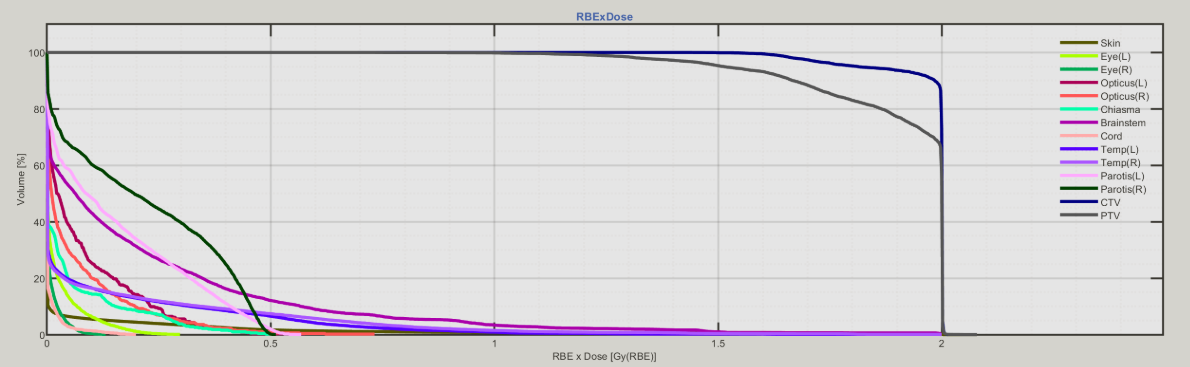
\includegraphics[width=0.6\textwidth]{images/carbon/carbon_best_DVH_graph.png}
                    \caption{Grafico DVH}
                    \label{fig:carbon_best_DVH_graph}
                \end{figure}
                \begin{table}[H]
                        \centering
                        \label{tab:dati_caso_clinico_carbon}
                        \begin{tabular}{
                            l | c | c | c | c | c |
                        }
                            \toprule
                            & Mean & Std & Max & Min & D$_{98}$ \\
                            \midrule
                            Skin & 0.0314 & 0.1730 & 2.0792 & 0 & 0 \\
                            Left eye & 0.0198 & 0.0425 & 0.2977 & 0 & 0 \\
                            Right eye & 0.0067 & 0.0160 & 0.1330 & 0 & 0 \\
                            Left opticus & 0.0751 & 0.1055 & 0.5773 & \num{3.1522e-07} & \num{1.8638e-06} \\
                            Right opticus & 0.0603 & 0.1060 & 0.7326 & 0 & 0 \\
                            Chiasma & 0.0437 & 0.0929 & 0.4993 & 0 & 0 \\
                            Brainstem & 0.1992 & 0.3195 & 1.9990 & 0 & 0 \\
                            Cord & 0.0054 & 0.0197 & 0.1997 & 0 & 0 \\
                            Left Temp & 0.0796 & 0.2077 & 1.9987 & 0 & 0 \\
                            Right Temp & 0.0893 & 0.2424 & 1.9999 & 0 & 0 \\
                            Left Parotis & 0.1514 & 0.1603 & 0.5690 & 0 & 0 \\
                            Right Parotis & 0.2139 & 0.1801 & 0.5124 & 0 & 0 \\
                            CVT & 1.9809 & 0.0713 & 2.0159 & 1.4445 & 1.6698 \\
                            PVT & 1.9161 & 0.1741 & 2.0792 & 0.6965 & 1.3260 \\
                            \bottomrule
                        \end{tabular}
                        \caption{Dati ottenuti dalle curve di isodose (unità di misura della tabella [\unit{\gray}])}
                    \end{table}    

        \subsection{Caso clinico con malposizionamento paziente}
            \subsubsection{Fotoni}
                \begin{figure}[H]
                    \centering
                    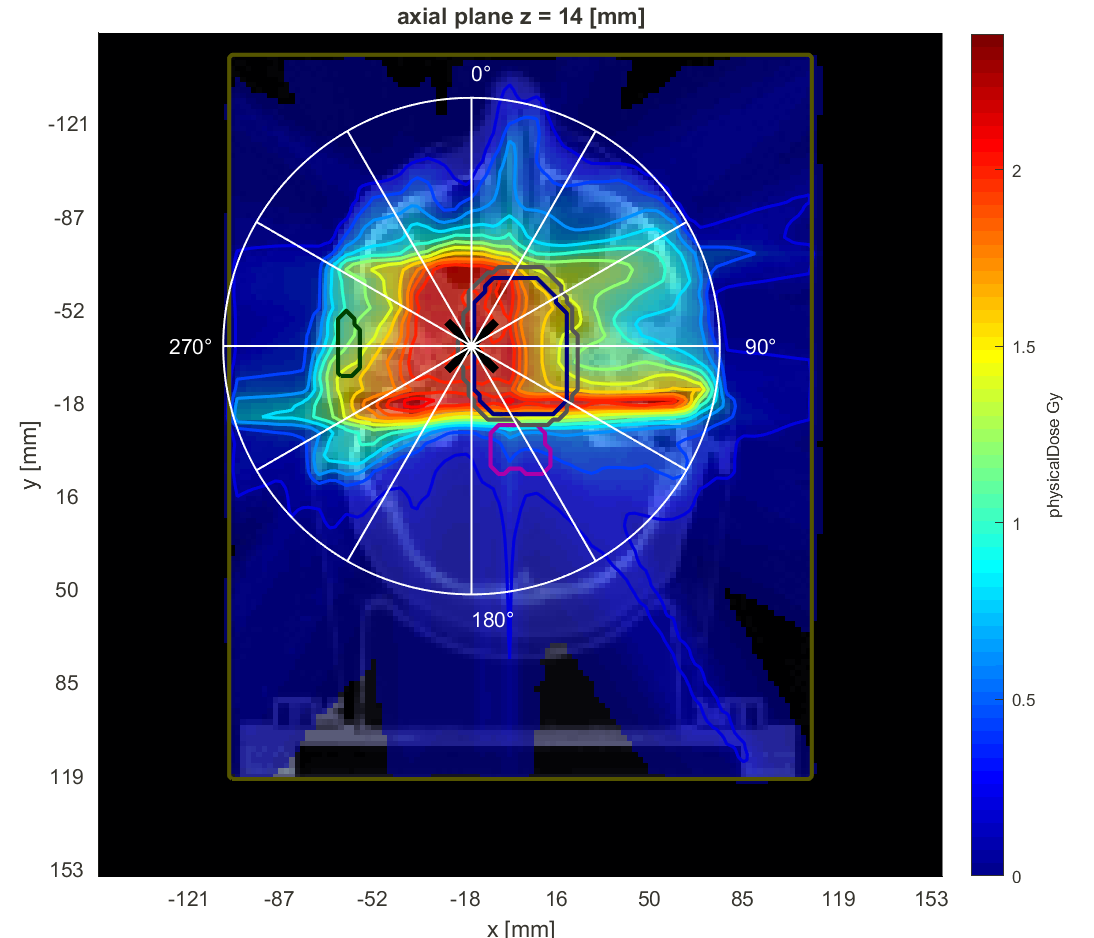
\includegraphics[width=0.6\textwidth]{images/photons/photons_worst_intensity.png}
                    \caption{Intensità fasci fotoni}
                    \label{fig:sub_fotoni_worst}
                \end{figure}
                \begin{figure}[H]
                    \centering
                    \begin{subfigure}{0.5\textwidth}
                        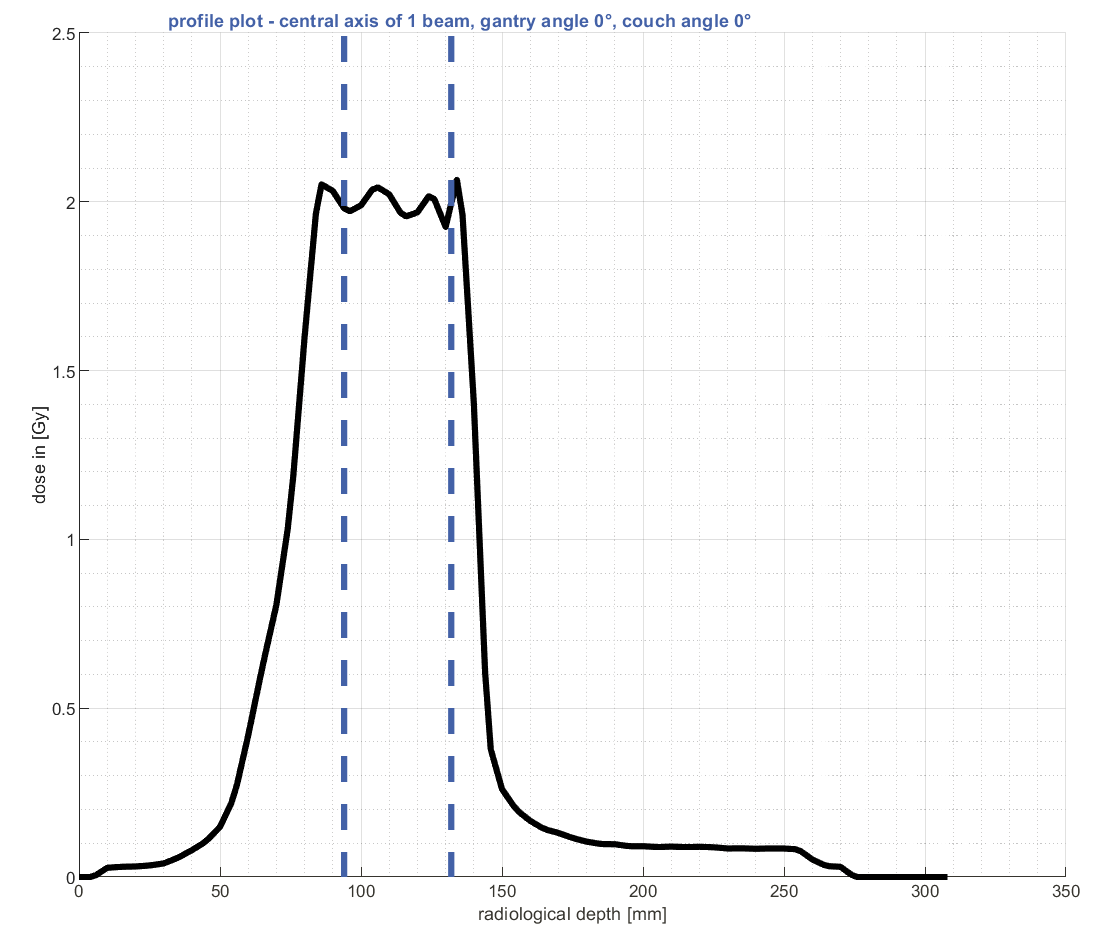
\includegraphics[width=\textwidth]{images/photons/photons_worst_depth.png}
                        \caption{Profilo depth}
                        \label{fig:sub_fotoni_worst_profile_depth}
                    \end{subfigure}\hfill
                    \begin{subfigure}{0.5\textwidth}
                        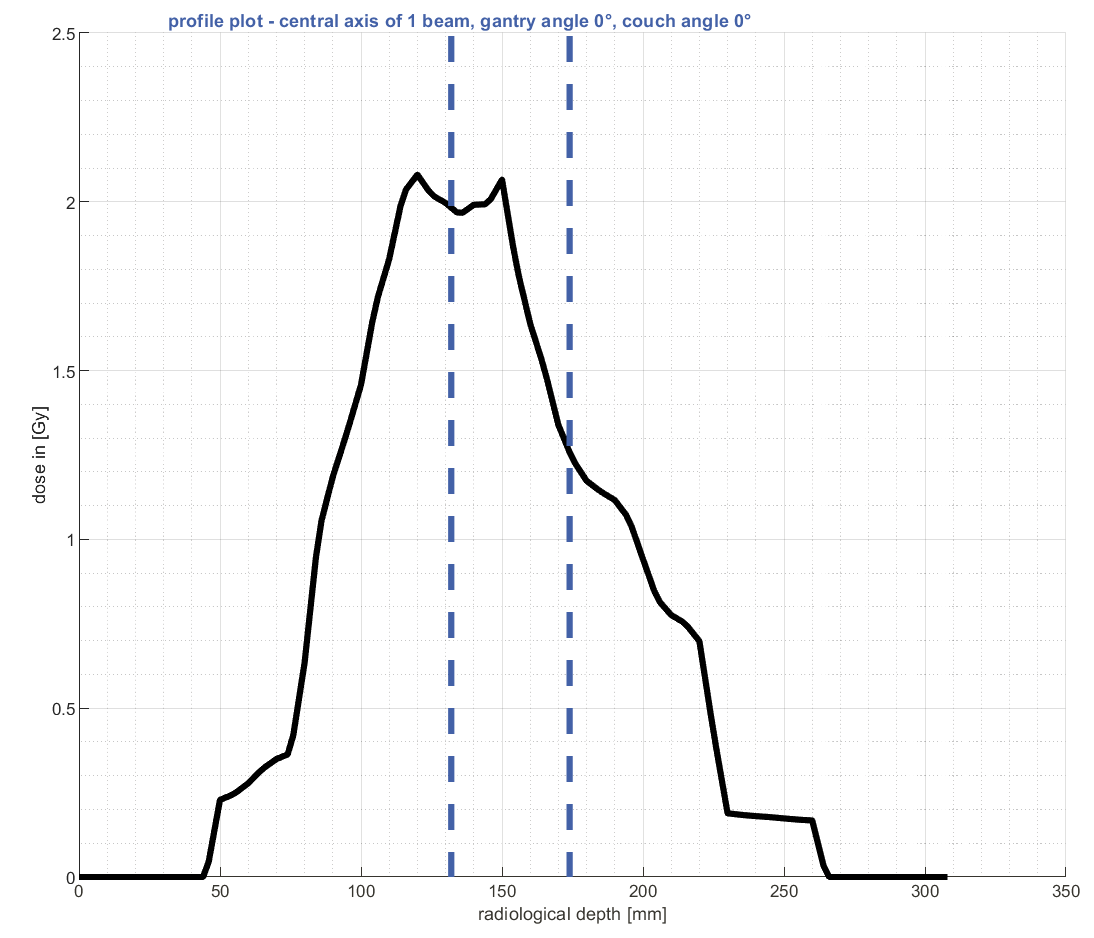
\includegraphics[width=\textwidth]{images/photons/photons_worst_lateral.png}
                        \caption{Profilo lateral}
                        \label{fig:sub_fotoni_worst_profile_lateral}
                    \end{subfigure}\hfill
                    \caption{Profili del fascio di fotoni}
                    \label{fig:fotoni_4_worst_profiles}
                \end{figure}
                \begin{figure}[H]
                    \centering
                    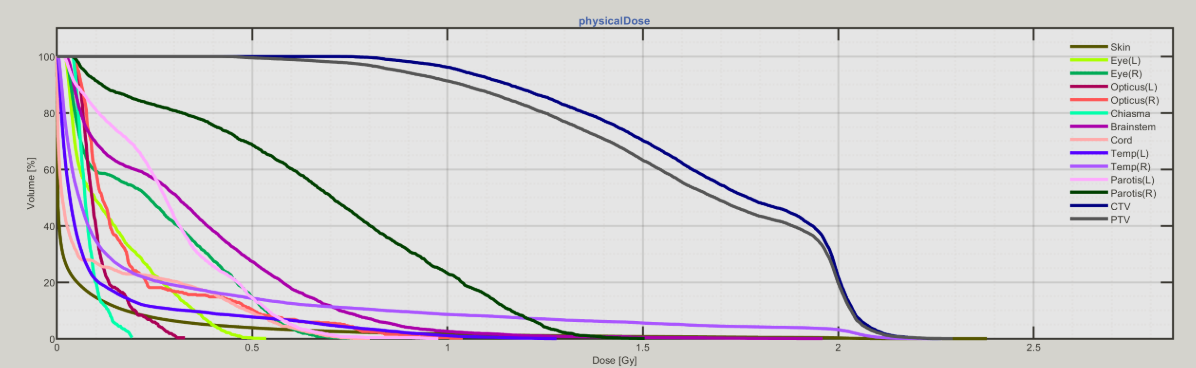
\includegraphics[width=0.6\textwidth]{images/photons/photons_worst_DVH_graph.png}
                    \caption{Grafico DVH}
                    \label{fig:fotoni_worst_DVH_graph}
                \end{figure}
                \begin{table}[H]
                        \centering
                        \label{tab:dati_malposizionamento_fotoni}
                        \begin{tabular}{
                            l | c | c | c | c | c |
                        }
                            \toprule
                            & Mean & Std & Max & Min & D$_{98}$\\
                            \midrule
                            Skin & 0.0725 & 0.2298 & 2.3816 & 0 & 0 \\
                            Left eye & 0.1474 & 0.1259 & 0.5372 & 0.0199 & 0.0242 \\
                            Right eye & 0.2501 & 0.1981 & 0.7623 & 0.0222 & 0.0266 \\
                            Left opticus & 0.1090 & 0.0598 & 0.3301 & 0.0403 & 0.0475 \\
                            Right opticus & 0.1963 & 0.1997 & 1.0396 & 0.0426 & 0.0484 \\
                            Chiasma & 0.0807 & 0.0329 & 0.1937 & 0.0405 & 0.0436 \\
                            Brainstem & 0.3446 & 0.2911 & 1.9606 & 0.0194 & 0.0315 \\
                            Cord & 0.1218 & 0.2004 & 0.8021 & 0 & 0 \\
                            Left Temp & 0.1129 & 0.2150 & 1.2795 & 0.0018 & 0.0036 \\
                            Right Temp & 0.2538 & 0.4846 & 2.2772 & 0.0031 & 0.0058 \\
                            Left Parotis & 0.2892 & 0.1793 & 0.9772 & 0.0172 & 0.0257 \\
                            Right Parotis & 0.6825 & 0.3658 & 1.5065 & 0.0397 & 0.0539 \\
                            CVT & 1.6885 & 0.3480 & 2.2631 & 0.7279 & 0.9102 \\
                            PVT & 1.6196 & 0.4000 & 2.2944 & 0.3933 & 0.7143 \\
                            \bottomrule
                        \end{tabular}
                        \caption{Dati ottenuti dalle curve di isodose (unità di misura della tabella [\unit{\gray}])}
                    \end{table}

            \subsubsection{Protoni}
                \begin{figure}[H]
                    \centering
                    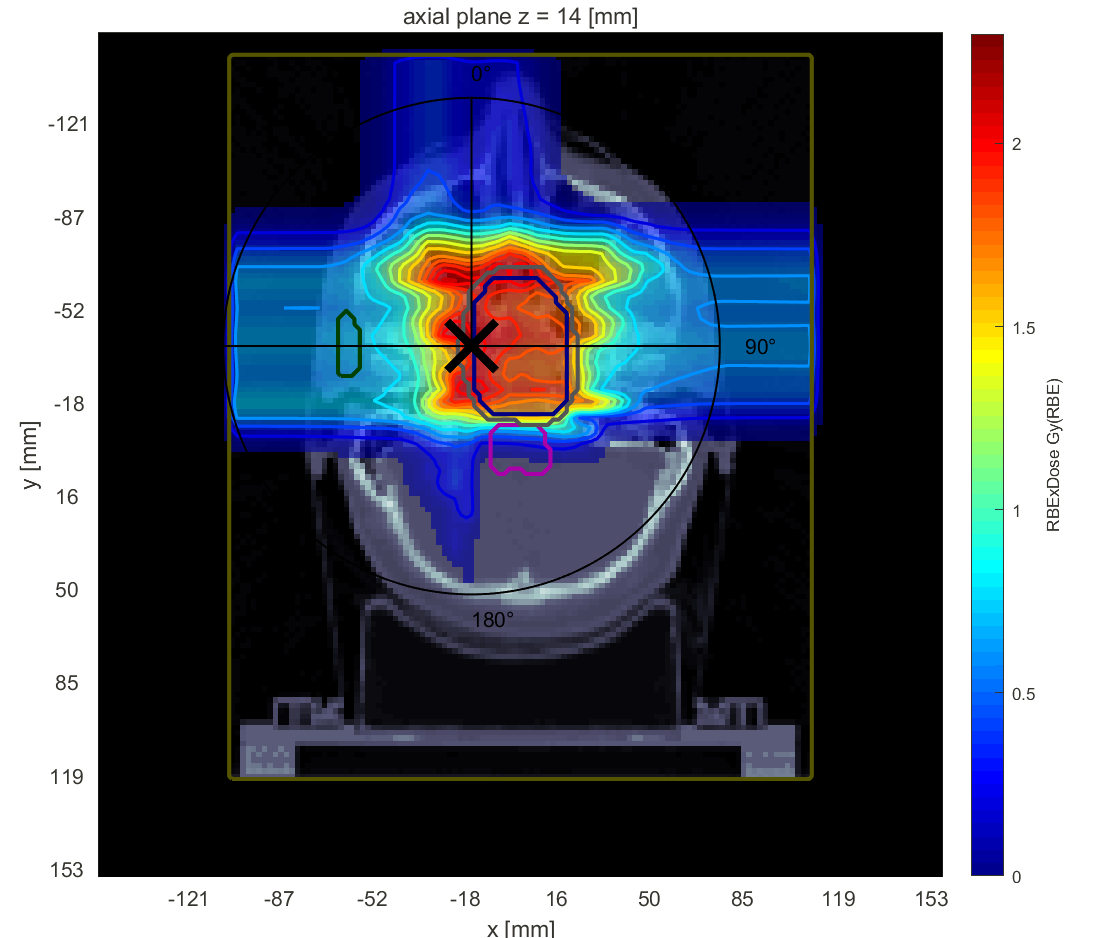
\includegraphics[width=0.6\textwidth]{images/protons/protons_worst_intensity.png}
                    \caption{Intensità fasci protoni}
                    \label{fig:sub_protoni_worst}
                \end{figure}
                \begin{figure}[H]
                    \centering
                    \begin{subfigure}{0.5\textwidth}
                        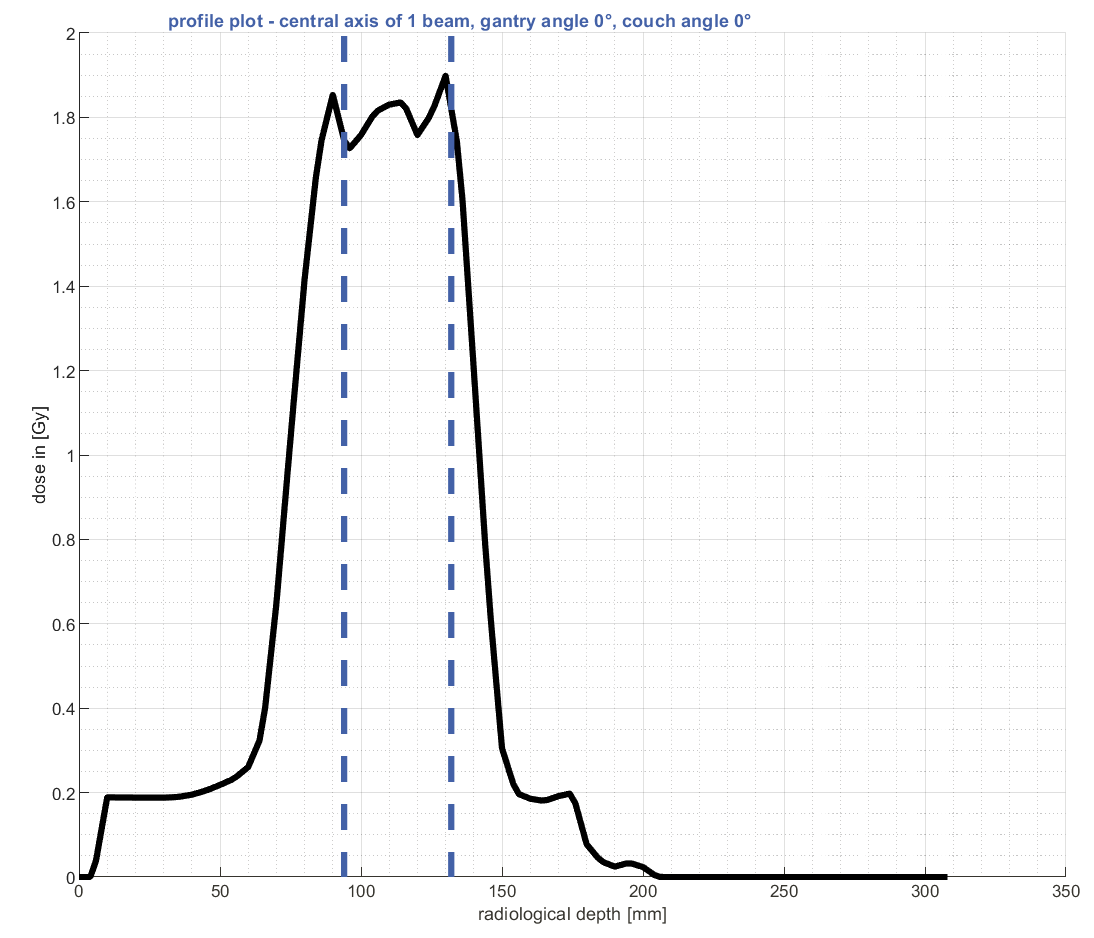
\includegraphics[width=\textwidth]{images/protons/protons_worst_depth.png}
                        \caption{Profilo depth}
                        \label{fig:sub_protoni_worst_profile_depth}
                    \end{subfigure}\hfill
                    \begin{subfigure}{0.5\textwidth}
                        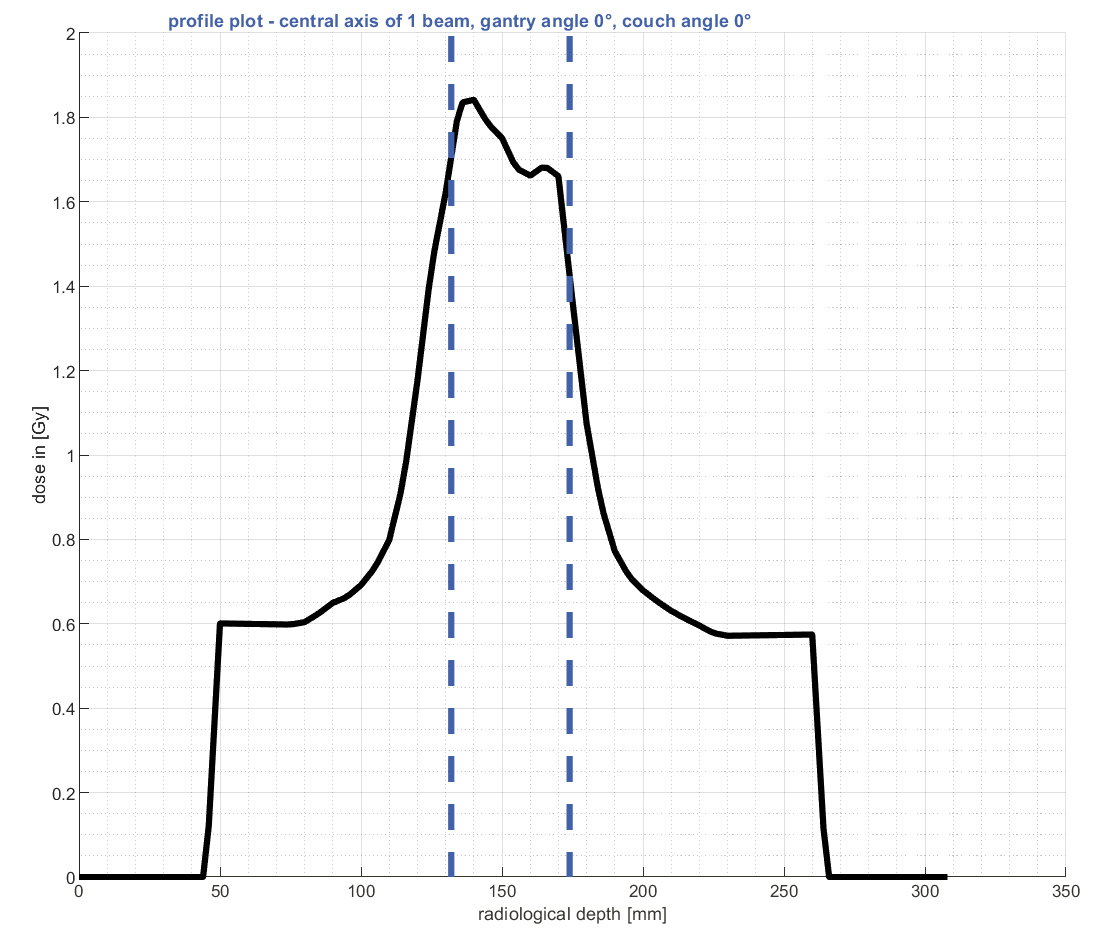
\includegraphics[width=\textwidth]{images/protons/protons_worst_lateral.png}
                        \caption{Profilo lateral}
                        \label{fig:sub_protoni_worst_profile_lateral}
                    \end{subfigure}\hfill
                    \caption{Profili dei fasci di protoni}
                    \label{fig:protoni_worst_profiles}
                \end{figure}
                \begin{figure}[H]
                    \centering
                    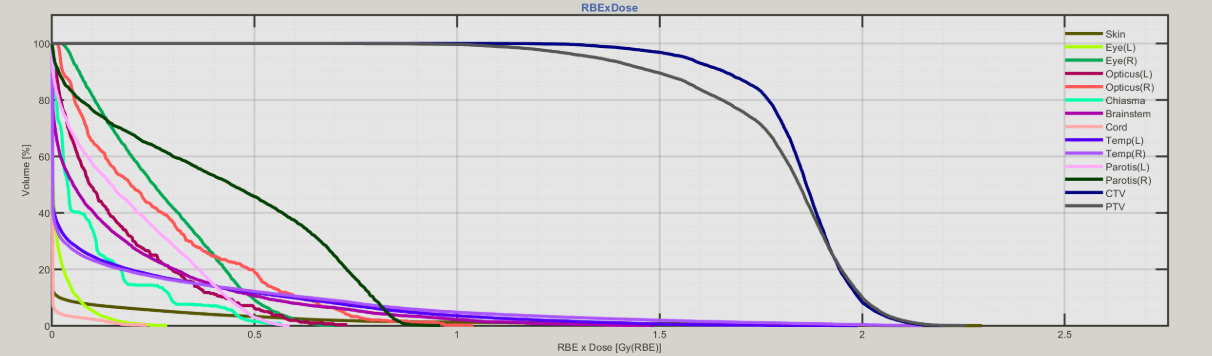
\includegraphics[width=0.6\textwidth]{images/protons/protons_worst_DVH_graph.png}
                    \caption{Grafico DVH}
                    \label{fig:protoni_worst_DVH_graph}
                \end{figure}
                \begin{table}[H]
                        \centering
                        \label{tab:dati_malposizionamento_protoni}
                        \begin{tabular}{
                            l | c | c | c | c | c |
                        }
                            \toprule
                            & Mean & Std & Max & Min & D$_{98}$\\
                            \midrule
                            Skin & 0.0452 & 0.2039 & 2.2965 & 0 & 0 \\
                            Left eye & 0.0195 & 0.0382 & 02860 & 0 & 0 \\
                            Right eye & 0.2688 & 0.1612 & 0.7092 & 0.0240 & 0.0380 \\
                            Left opticus & 0.1603 & 0.1658 & 0.7292 & \num{8.0109e-04} & 0.0025 \\
                            Right opticus & 0.2616 & 0.2282 & 1.0413 & 0.0129 & 0.0177 \\
                            Chiasma & 0.0997 & 0.1302 & 0.5699 & 0.0014 & 0.0023 \\
                            Brainstem & 0.1713 & 0.2591 & 1.4846 & 0 & \num{1.5684e-08} \\
                            Cord & 0.0048 & 0.0248 & 0.2343 & 0 & 0 \\
                            Left Temp & 0.1438 & 0.3067 & 1.9891 & 0 & 0 \\
                            Right Temp & 0.1566 & 0.3605 & 2.1483 & 0 & 0 \\
                            Left Parotis & 0.1854 & 0.1646 & 0.5870 & 0 & \num{6.6093e-05} \\
                            Right Parotis & 0.4179 & 0.2934 & 0.9600 & \num{7.1538e-05} & 0.0018 \\
                            CVT & 1.8430 & 0.1419 & 2.2005 & 1.0896 & 1.4337 \\
                            PVT & 1.7917 & 0.2135 & 2.2591 & 0.6916 & 1.1898 \\
                            \bottomrule
                        \end{tabular}
                        \caption{Dati ottenuti dalle curve di isodose (unità di misura della tabella [\unit{\gray}])}
                    \end{table}

            \subsubsection{Ioni carbonio}
                \begin{figure}[H]
                    \centering
                    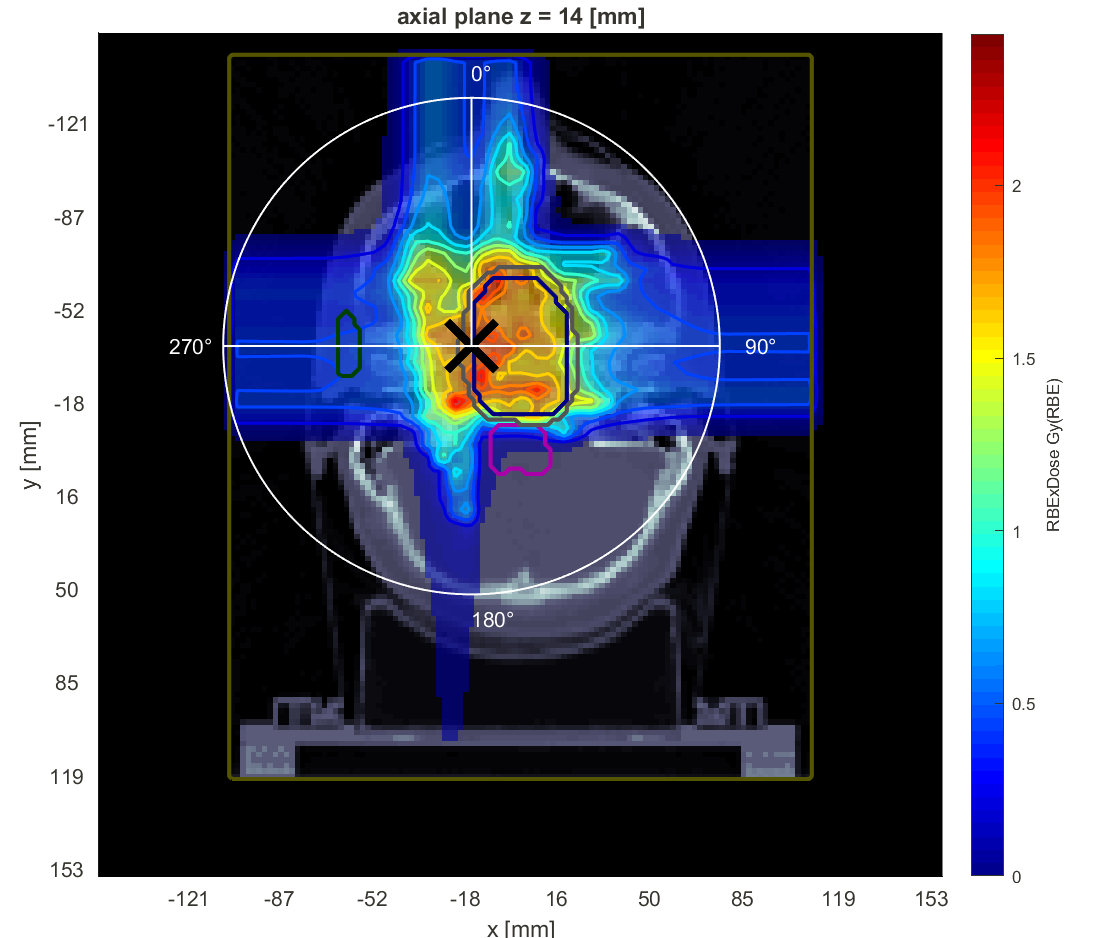
\includegraphics[width=0.6\textwidth]{images/carbon/carbon_worst_intensity.png}
                    \caption{Intensità fasci ioni carbonio}
                    \label{fig:carbonio_worst}
                \end{figure}
                \begin{figure}[H]
                    \centering
                    \begin{subfigure}{0.5\textwidth}
                        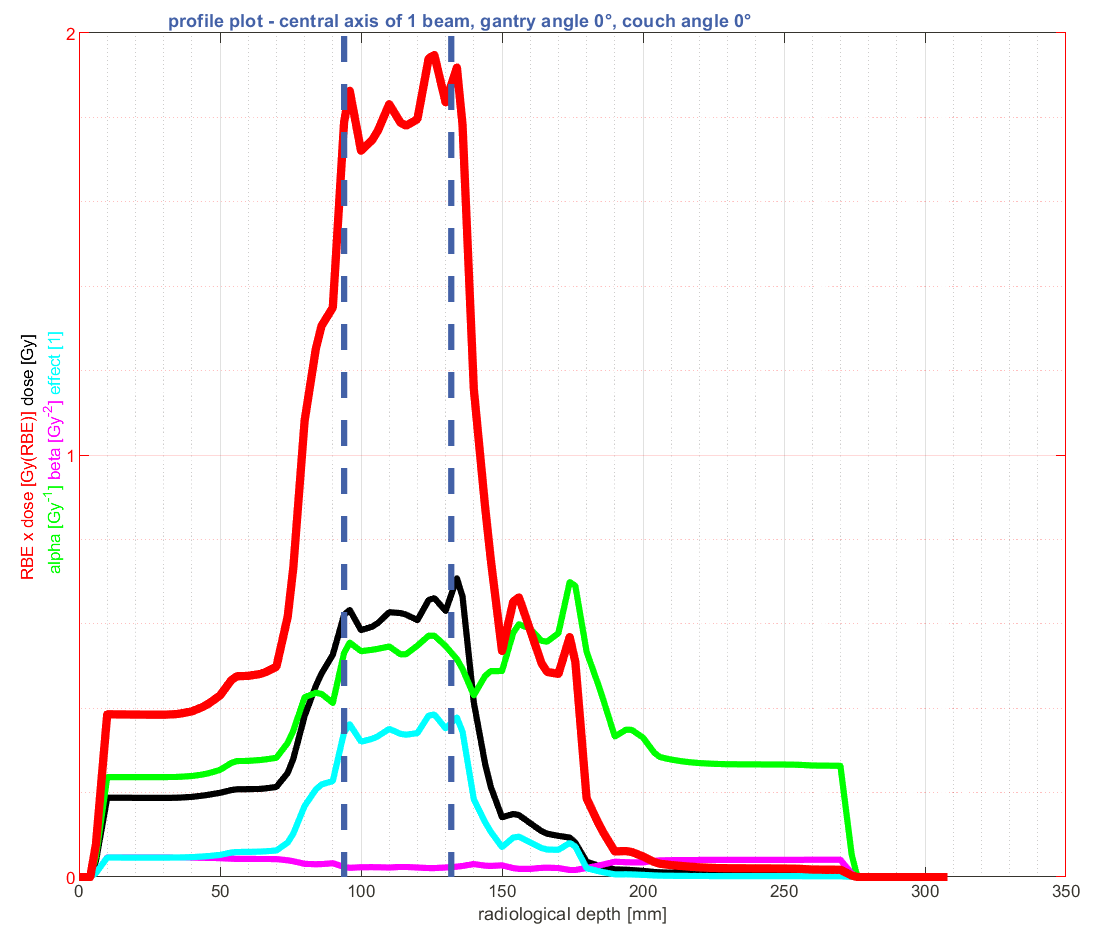
\includegraphics[width=\textwidth]{images/carbon/carbon_worst_depth.png}
                        \caption{Profilo depth}
                        \label{fig:sub_carbonio_worst_profile_depth}
                    \end{subfigure}\hfill
                    \begin{subfigure}{0.5\textwidth}
                        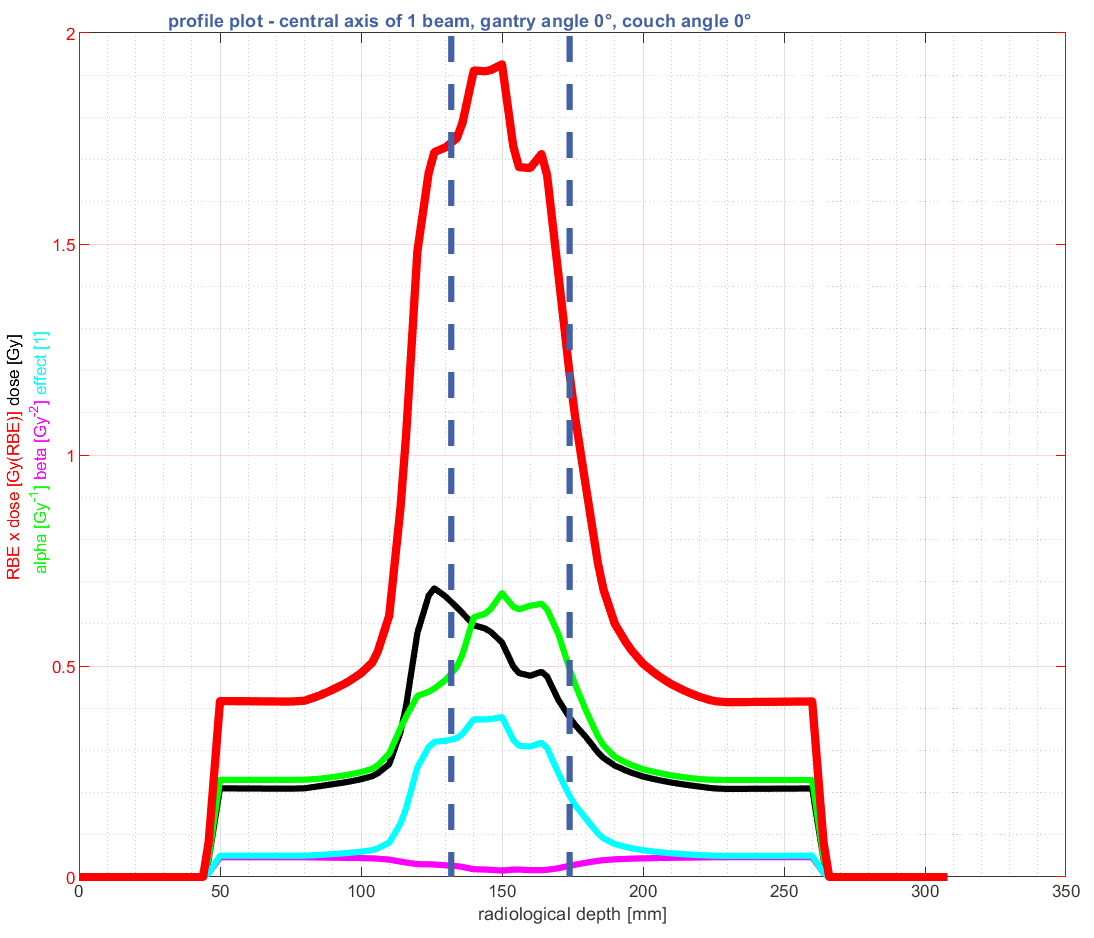
\includegraphics[width=\textwidth]{images/carbon/carbon_worst_lateral.png}
                        \caption{Profilo lateral}
                        \label{fig:sub_carbonio_worst_profile_lateral}
                    \end{subfigure}\hfill
                    \caption{Profili del fascio di ioni carbonio}
                    \label{fig:carbonio_worst_profiles}
                \end{figure}
                \begin{figure}[H]
                    \centering
                    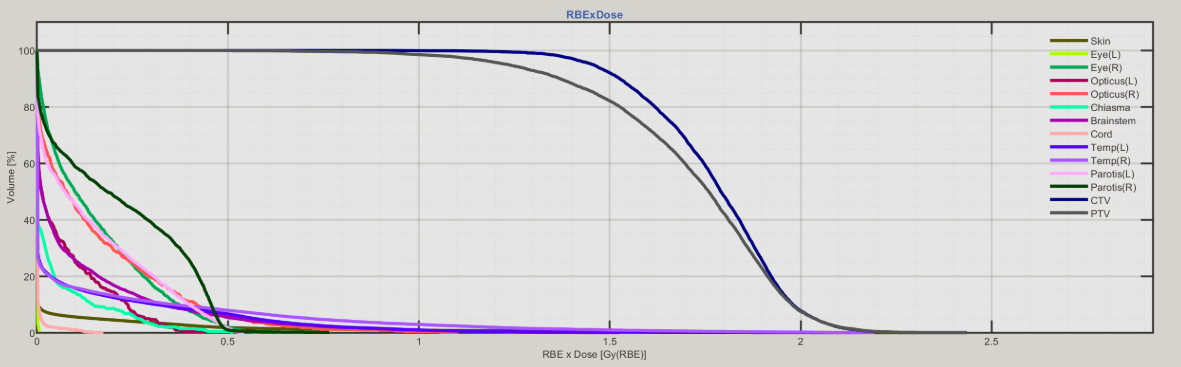
\includegraphics[width=0.6\textwidth]{images/carbon/carbon_worst_DVH_graph.png}
                    \caption{Grafico DVH}
                    \label{fig:carbon_worst_DVH_graph}
                \end{figure}
                \begin{table}[H]
                        \centering
                        \label{tab:dati_malposizionamento_carbon}
                        \begin{tabular}{
                            l | c | c | c | c | c |
                        }
                            \toprule
                            & Mean & Std & Max & Min & D$_{98}$ \\
                            \midrule
                            Skin & 0.0317 & 0.1690 & 2.4362 & 0 & 0 \\
                            Left eye & \num{2.5399e-04} & \num{9.7829e-04} & 0.0101 & 0 & 0 \\
                            Right eye & 0.1484 & 0.1445 & 0.6227 & 0 & 0 \\
                            Left opticus & 0.0677 & 0.0987 & 0.4389 & 0 & 0 \\
                            Right opticus & 0.1522 & 0.1896 & 1.1043 & 0 & \num{2.6312e-08} \\
                            Chiasma & 0.0415 & 0.0896 & 0.5169 & 0 & \num{2.5721e-08} \\
                            Brainstem & 0.1017 & 0.1966 & 1.5274 & 0 & 0 \\
                            Cord & 0.0030 & 0.0149 & 0.1752 & 0 & 0 \\
                            Left Temp & 0.0784 & 0.2096 & 2.1450 & 0 & 0 \\
                            Right Temp & 0.1005 & 0.2863 & 2.1964 & 0 & 0 \\
                            Left Parotis & 0.1412 & 0.1571 & 0.5448 & 0 & 0 \\
                            Right Parotis & 0.2111 & 0.1833 & 0.7665 & 0 & 0 \\
                            CVT & 1.7722 & 0.1810 & 2.4362 & 0.9441 & 1.3699 \\
                            PVT & 1.7105 & 0.2511 & 2.4362 & 0.4835 & 1.0684 \\
                            \bottomrule
                        \end{tabular}
                        \caption{Dati ottenuti dalle curve di isodose (unità di misura della tabella [\unit{\gray}])}
                    \end{table}    

    % -------------------------------------------------------------------
    \section{Conclusioni}
        Si osserva la differenza nel deposito di energia tra fotoni, protoni e ioni carbonio. 
        I fotoni, quando entrano nei tessuti, depositano energia con una decrescita esponenziale.
        I protoni e gli ioni carbonio invece depositano energia in maniera più mirata.
        Questo è dovuto ai diversi metodi di interazione delle particelle con la materia: i fotoni interagiscono solo tramite effetto compton, effetto fotoelettrico e creazione di coppie, mentre protoni e ioni carbonio depositano energia seguendo la formula di Bethe-Block.
        Una differenza tra protoni e ioni carbonio è il fatto che gli ioni carbonio una volta che depositano buona parte della loro energia si dividono nelle loro componenti elementari che continuano a ionizzare i tessuti.
        Aumentando il numero di fasci si riesce a fare in modo che i fasci liberino energia più nel target e meno nell'organo a rischio.
        Inoltre si può osservare come il caso con i fasci non equidistanziati sia leggermente migliore rispetto a quello non equidistanziato, poiché i fasci non sono costretti ad attraversare direttamente l'organo a rischio, ma sono tutti concentrati in direzione del target.
        Scambiando organo a rischio e target si osserva, come previsto, che MatRad ottimizza i fasci in modo da depositare energia sul nuovo target.
        \\
        Nel caso clinico, grazie a quanto studiato precedentemente, si sono scelte le configurazioni più efficaci per colpire il target preservando nel contempo gli organi più delicati.
        Siccome i fotoni depositano energia in maniera meno mirata pertanto, gli organi circostanti assorbono necessariamente una certa dose di radiazione per quasi tutta la totalità del loro volume.
        Invece protoni e ioni carbonio, riuscendo a depositare energia in maniera più mirata sulla massa tumorale, consentono un minor assorhimento di dose da parte degli altri organi.
        Nel caso di un malposizionamento del paziente si osserva come in tutti e tre i casi aumenti la dose di radiazione assorbita dagli organi a rischio e diminuisca quella depositata sul tumore.

\end{document}